\documentclass[minted, notitle]{protocol}
% Packages
\usepackage{enumitem}
\usepackage{verbatim}
%\documentclass[xcolor=dvipsnames]{beamer} 
\usepackage{pgfmath}
\usepackage{sectsty}
\usepackage{booktabs}% http://ctan.org/pkg/booktabs
\newcommand{\tabitem}{~~\llap{\textbullet}~~}
\usepackage{tabularx}
\usepackage{rotating}
\usepackage{colortbl} % Bunte hlines
\usepackage{makecell}


\usepackage{array, boldline, makecell, booktabs}
\newcommand\btrule[1]{\specialrule{#1}{0pt}{0pt}}


%\usepackage{paralist}
%\usepackage{enumerate}
%\usepackage{enumitem}
%\usepackage{enumitem,showframe}

\usepackage{tikz}        

\newcommand\mybox[3][]{%
    \tikz[anchor=base,baseline]\node[inner sep=2pt,draw=#2,#1]{$\displaystyle#3\mathstrut$};}
\colorlet{mycol}{white}



% Optional
% \mysubtitle{Lastenheft}
% \mysubject{Systemtechnik Labor}
%\mycourse{xHIT 2017/18, Gruppe A}
% Version
% \myteacher{}

%\mybegin{31. Januar 2018}
%\myfinish{17. April 2018}
% \setcode{frame=single} 			% Add a frame to codes (single, lines)
% \setcode{bgcolor=MyLightGray}		% Add a background to codes (minted only)
% \usemintedstyle{rainbow_dash} 	% autumn, rainbow_dash, tango (default), trac
\tocfalse
\definecolor{celadon}{rgb}{0.67, 0.88, 0.69}
\definecolor{lightgrey}{rgb}{0.88 0.88 0.88}
%\definecolor{rlightgreen}{RGB}{221, 246, 202}
\definecolor{rlightgreen}{RGB}{242, 255, 230}
%\rowcolors{2}{celadon}{green!70!yellow!40}

\newcommand{\draft}{\cellcolor{Peach} Draft}
\newcommand{\abgabe}{\cellcolor{LimeGreen}Approved } 
\newcommand{\version}{1.0}

% Kacpers total wichtige Design-Prinzipien
\usepackage[sfdefault]{roboto} % The font, that beats them all...
% Farbensetzen für Sections
\sectionfont{\color{darkgray}}  % Green Hulk > Red Hulk
\subsectionfont{\color{gray}}
\subsubsectionfont{\color{gray}}
% Ich f*%!-/? liebe Tabellen
%\rowcolors{2}{rlightgreen}{white} Verwenden, falls man in einer Tabelle
\newcolumntype{A}[1]{>{\columncolor{rlightgreen}}p{#1}} % Kolumnentyp, für leichte grüne Farbe im Hintergrund 
% Jeder mag doch grüne Bullet Points oder?
\newlist{coloritemize}{itemize}{1}
\setlist[coloritemize]{label=\textcolor{OliveGreen}{\textbullet}}

% Wichtige Variablen, die das Dokument beschreiben:
\title{Lernbüroverwaltungstool} % Projektname mit \thetitle value holen
\newcommand{\subtitle}{some random text}
\myversion{1.4} % Version
\newcommand{\theversion}{1.4} % Bitte nochmal Version eintragen
\newcommand{\authors}{Kisser Manuel, Urbaniec Kacper, Welsch Moritz, Wustinger Martin} % Projektteam
\newcommand{\leader}{Kacper Urbaniec} % Projektleiter
\date{17.01.2019} % Datum
%\newcommand{\thedate}{14.11.2018} % Alles muss zweimal angegeben werden

\begin{document}
\begin{titlepage} % Fancy title page
	\raggedleft % Right align the title page
	
	\begingroup \color{gray}{\rule{3pt}{\textheight}} \endgroup % Vertical line
	\hspace{0.05\textwidth} % Whitespace between the vertical line and title page text
	\parbox[b]{0.75\textwidth}{ % Paragraph box for holding the title page text, adjust the width to move the title page left or right on the page
		{{\fontsize{27}{48} \selectfont  Projekthandbuch}} \\	\vspace{0.146\textheight} \\
		
		{
\includegraphics[width=220]{images/Logo_1.png}} \\[2\baselineskip]
		%{{\fontsize{65}{48} \bfseries \color{LimeGreen} LBVT}} \\[0.5\baselineskip] %\LaTeX ~Templates}\\[2\baselineskip] % Title
		{{\fontsize{20}{48} \selectfont \thetitle}} \\ %[0.5\baselineskip] % Subtitle or further description
		%{\Large Lernbüroverwaltungstool}\\ [2\baselineskip] % Subtitle or further description
		{\vspace{-0.5cm}\large \begin{flushleft}Kisser Manuel, Urbaniec Kacper, Welsch Moritz, \\Wustinger Martin\end{flushleft}}\\ [1\baselineskip]
		
		{\vspace{0.3cm}\large Version: \theversion}\\ [0.5\baselineskip] % Author name
		{\large Projektleiter: \leader}\\ [0.5\baselineskip] % Author name
		{\large Datum: \thedate}\\ [1\baselineskip] % Author name
		
		%\vspace{0.5\textheight} % Whitespace between the title block and the publisher
		
		{
\includegraphics[width=220]{images/tgm_full.png}}
		%{\noindent The Publisher~~\plogo}\\[\baselineskip] % Publisher and logo
	}
\end{titlepage}

% \thispagestyle{fancy}				% Makes the first page fancy too
% \begin{abstract}\end{abstract} 	% Add a short overview
%%!TEX root=../protocol.tex	% Optional

\section{Einführung}
Diese Protokollvorlage soll helfen den Laborübungsteil entsprechend dokumentieren zu können. Diese Vorlage ist in \LaTeX ~verfasst.

\subsection{Ziele}
Hier werden die zu erwerbenden Kompetenzen und deren Deskriptoren beschrieben. Diese werden von den unterweisenden Lehrkräften vorgestellt.

Dies kann natürlich auch durch eine Aufzählung erfolgen:
\begin{itemize}
	\item Dokumentiere wichtige Funktionen
	\item Gib eine Einführung zur Verwendung von \LaTeX
\end{itemize}

\subsection{Voraussetzungen}
Welche Informationen sind notwendig um die Laborübung reibungslos durchführen zu können? Hier werden alle Anforderungen der Lehrkraft detailliert beschrieben und mit Quellen untermauert.

\subsection{Aufgabenstellung}
Hier wird dann die konkrete Aufgabenstellung der Laborübung definiert.

\subsection{Bewertung}
Hier wird die Bewertung für das Beispiel auf die jeweiligen Kompetenzen aufgeteilt. Diese soll zur leichteren Abnahme auch nicht entfernt werden.
\\\\
Nun kommt ein Seitenumbruch, um eine klare Trennung der Schülerarbeit zu bestimmen. 	% Information about the purpose of this project
%%!TEX root=../protocol.tex	% Optional



\section{Konfiguration}
\subsection{Optionen}
\begin{tabularx}{\textwidth}{l X}
{\small \verb|landscape|}    & Richte das Dokument vertikal aus.\\
{\small \verb|minted|}       & Nutze das \texttt{minted} Paket zur Quelltextdarstellung.\\
{\small \verb|natbib|}       & Nutze NatBib zur Literaturverwaltung.\\
{\small \verb|nobib|}        & Deaktiviere die Literaturverwaltung.\\
{\small \verb|nofonts|}      & Nutze die Standard \LaTeX ~Schriftarten.\\
{\small \verb|noglo|}        & Deaktiviere Akronyme und das Glossar.\\
{\small \verb|nologos|}      & Zeichne keine Logos auf der Titelseite.\\
{\small \verb|notitle|}      & Zeichne keine Titelseite.\\
{\small \verb|notoc|}        & Zeichne kein Inhaltsverzeichnis.\\
{\small \verb|notable|}      & Zeichne keine Tabelle auf der Titelseite.
\end{tabularx}

\subsection{Variablen}
Variablen werden über Kommandos gesetzt, die als Parameter den gewünschten Wert erhalten.
\begin{center}
    \ifminted   \codein{tex}{\myvariable{value}}
    \else       \codein{tex}{\\myvariable\{value\}}\fi
\end{center}

\begin{tabular}{l l}
\textbf{Kommando} & \textbf{Inhalt}\\

{\small \verb|mysubtitle|} 	& Untertitel oder Zugehörigkeit\\
{\small \verb|mysubject|} 	& Thema / Fach, welches bearbeitet wird\\
{\small \verb|mycourse|} 	& Kurs / Klasse welche(r) besucht wird\\
{\small \verb|myteacher|} 	& Betreuende Lehrkraft\\
{\small \verb|myversion|} 	& Aktuelle Version des Dokuments\\
{\small \verb|mybegin|} 	& Datum des Beginns\\
{\small \verb|myfinish|} 	& Datum an dem die Arbeit beendet wurde
\end{tabular}

\newpage
\section{Kommandos}\label{sec:Kommandos}
\subsection{\texttt makefig}

\begin{listing}
\begin{code}{tex}
\makefig{images/logo-right.png}{height=2cm}{
    Mit Beschreibung und Label  % (Optional)
}{
    fig:caption-label           % (Optional)
}
\end{code}
\caption{\texttt makefig}
\label{lst:makefig}
\end{listing}
\makefig{images/logo-right.png}{height=2cm}{Mit Beschreibung und Label}{fig:caption-label}

\subsection{\texttt vardef}
\begin{listing}
\begin{code}{tex}
$$e^{i*\pi} = -1$$
\end{code}

$$e^{i*\pi} = -1$$

\begin{code}[firstnumber=last]{tex}
\begin{vardef}
    \addvardef{$e$}{Eulersche Zahl}
    \addvardef{$\pi$}{Kreiszahl}
    \addvardef{$i$}{Imagin\"are Einheit}
\end{vardef}
\end{code}

\begin{vardef}
    \addvardef{$e$}{Eulersche Zahl}
    \addvardef{$\pi$}{Kreiszahl}
    \addvardef{$i$}{Imaginäre Einheit}
\end{vardef}

\caption{\texttt vardef}
\label{lst:vardef}
\end{listing}

\newpage
\section{Anwendung}\label{sec:Anwendung}
Hier sollen die Schritte der Laborübung erläutert werden. Hier sind alle Fragestellungen der Lehrkraft zu beantworten. Etwaige Probleme bzw. Schwierigkeiten sollten ebenfalls hier angeführt werden.

In diesem Fall werden einige \LaTeX-Elemente dokumentiert, welche bei der Kreation von Protokollen behilflich sein könnten.

\subsection{Tabellen}
\begin{table}[H]
	\center
	\begin{tabular}{| c | l |}
		\hline Header 	& Kopf\\ \hline\hline
		\textbf{Lorem} 	& Ipsum dolor sit amet, consetetur sadipscing elitr\\ \hline
		\textbf{Ipsum} 	& At vero eos et accusam et justo duo dolores et ea rebum.\\
						& Stet clita kasd gubergren, no sea takimata sanctus\\ \hline
		\textbf{Dolor} 	& Consetetur sadipscing elitr, sed diam nonumy\\\hline
	\end{tabular}
	\caption{Tabular}
	\label{tab:tabular}
\end{table}

\subsubsection{TabularX}
TabularX erlaubt die Angabe der Größe der Tabelle und bietet zudem den Reihentyp \texttt{X}, der die verbleibende Größe neben anderen Reihen mit anderen \texttt{X} Reihen teilt.
\\\\
ACHTUNG: Die Verwendung von \verb|\codein|, \verb|\mintinline| oder \verb|\lstinline| ist in einer TabularX Umgebung nicht möglich!
\begin{table}
    \center
    \begin{tabularx}{\textwidth}{| c | X |}
        \hline Header 	& Kopf\\ \hline\hline
        \textbf{Lorem} 	& Ipsum dolor sit amet, consetetur sadipscing elitr\\ \hline
        \textbf{Ipsum} 	& At vero eos et accusam et justo duo dolores et ea rebum.\\
            			& Stet clita kasd gubergren, no sea takimata sanctus\\ \hline
        \textbf{Dolor} 	& Consetetur sadipscing elitr, sed diam nonumy\\\hline
    \end{tabularx}
    \caption{TabularX}
    \label{tab:tabularx}
\end{table}

\newpage
\subsection{Aufzählung}
\begin{itemize}
	\item Element einer Aufzählung
	\begin{itemize}
        \item Erstes eingerücktes Element einer Aufzählung
        \item Zweites eingerücktes Element einer Aufzählung
    \end{itemize}
\end{itemize}

\subsubsection{Outlines}
\begin{outline}
    \1 Element einer Aufzählung
        \2 Erstes eingerücktes Element einer Aufzählung
        \2 Zweites eingerücktes Element einer Aufzählung
\end{outline}

\subsection{Glossar}
Zur Verwaltung des Glossars wird standardmäßig die Datei \texttt{glossaries.tex} verwendet, wobei sowohl Definitionen als auch Akronyme definiert werden können.
\\\\
Als Beispiel wurde ein Akronym für \gls{ac-syt} und eine Definition zu \gls{ac-syt} selbst hinzugefügt.

\begin{listing}
\inputcode{tex}{glossaries.tex}
\caption{Glossareintrag}
\label{lst:glossaries}
\end{listing}
~\\
Im Dokument selbst kann ein Akronym mittels \verb|\gls{ac-syt}| verwendet werden. Beachte, dass ein Akronym welches bereits im Dokument verwendet wurde, bei der ersten Verwendung ausgeschrieben und danach immer gekürzt wird.
\\\\
Mit \verb|\gls{syt}| kann zum Beispiel eine Referenz zur Definition von \gls{syt} hinzugefügt werden.

\subsection{Zitate}
Zitate sollten gesammelt in der Datei \texttt{bib.bib} verwaltet werden.

\newpage
\subsection{Quelltext}
\begin{listing}
\ifminted   \mint{tex}|\begin{code}[]{java}|    % Escape \ for lstlistings
\else       \lstinline[numbers=left, language=tex]$\begin{code}[]{java}$\fi
\begin{code}[firstnumber=last]{java}
// Ich bin ein Kommantar!
public static void main(String[] args) {
    System.out.println("Ich bin ein Array!")
}
\end{code}
\ifminted   \mint[firstnumber=last]{tex}|\end{code}|    % Escape \ for lstlistings
\else       \lstinline[firstnumber=last, numbers=left, language=tex]$\end{code}$\fi

\caption{Java Code}
\label{lst:java-code}
\end{listing}
~\\
Die Darstellung von Quelltext im Text ist über das Kommando \verb|\codein[options]{lang}{code}| möglich.

\subsubsection{Listings}
\begin{listing}
\ifminted   \mint{tex}|\begin{lstlisting}[language=Java, caption=Java Lstlisting]|
\else       \lstinline[numbers=left, language=tex]$\begin{lstlisting}[language=Java, caption=Java Lstlisting]$\fi
\begin{code}[firstnumber=last]{java}
// Ich bin ein Kommantar!
public static void main(String[] args) {
    System.out.println("Ich bin ein Array!")
}
\end{code}
\ifminted   \mint[firstnumber=last]{tex}|\end{lstlisting}|
\else       \lstinline[firstnumber=last, numbers=left, language=tex]$\end{lstlisting}$\fi
\caption{Java Lstlisting}
\label{lst:java-lstlisting}
\end{listing}

\newpage
\subsubsection{Minted}
Benötigt die Option \texttt{minted}.
\paragraph{Umgebung}~\\
\begin{listing}
\ifminted   \mint{tex}|\begin{minted}[options]{java}|
\else       \lstinline[numbers=left, language=tex]$\begin{minted}[]{java}$\fi
\begin{code}[firstnumber=last]{java}
// Ich bin ein Kommantar!
public static void main(String[] args) {
    System.out.println("Ich bin ein Array!")
}
\end{code}
\ifminted   \mint[firstnumber=last]{tex}|\end{minted}|
\else       \lstinline[firstnumber=last, numbers=left, language=tex]$\end{minted}$\fi
\caption{Minted Umgebung}
\label{lst:minted-env}
\end{listing}

\paragraph{Zeile}~\\
\begin{listing}
\ifminted   \mint{tex}$\mint[options]{lang}|code|$
\else       \lstinline[language=tex]$\mint[options]{lang}|code|$\fi
\caption{Minted Einzeiler}
\label{lst:minted-line}
\end{listing}

\begin{listing}
\begin{code}{tex}
\mintinline[options]{lang}{code}
\end{code}
\caption{Minted Inline}
\label{lst:minted-inline}
\end{listing} % Solution for the given tasks and their documentation
% \glsaddall 		% Add all glossary entries to printglossaries



\clearpage
{ % Wir wollen ja kein blaues Inhaltsverzeichnis :), im blue da ba dee
  \hypersetup{linkcolor=black}
  \tableofcontents
} 
\clearpage


%!TEX root=../protocol.tex	% Optional

% Für Aufzählungen im Dokument wichtig!
\setlist[itemize]{itemindent=0em, topsep=0pt, noitemsep, leftmargin=0.15in}
% Immer zwischen begin[{itemize} und end{itemize} angeben!!!
\newcommand{\vb}{\vspace{-0.2cm}}
\newcommand{\vt}{\vspace{-0.3cm}}


%%%%%%%%%%%%%%%%%%%%%%%%%%%%%%%%%%%%%%%%%%%%%%%%%%%%%%%%%%%%%%%%%%%%%%%%%%%%%%%%%%%%%
%                                                                                   %
%   WICHTIG, bei \item, das nachfolgende \text{} Feld IMMER löschen!                %
%   Dient nur zum Anzeigen der Bullet-Points, falls kein Text gesetzt ist           %
%                                                                                   %  
%%%%%%%%%%%%%%%%%%%%%%%%%%%%%%%%%%%%%%%%%%%%%%%%%%%%%%%%%%%%%%%%%%%%%%%%%%%%%%%%%%%%%

\section*{Änderungsverzeichnis}
\begin{center}
\rowcolors{2}{white}{white}
\begin{tabularx}{\textwidth}{| l | p{1.8cm} | l | X |}
\hline \rowcolor{gray} \textbf{\color{white}Version} & \textbf{\color{white}Autor} & \textbf{\color{white}Datum} &  \textbf{\color{white}Änderung} \\ 
 \hline \hline
 0.1 & Kacper Urbaniec & 25.10.2018 & Projektauftrag, Projektumweltanalyse\\
 \hline
 0.2 & Martin Wustinger & 25.10.2018 & Projektzieleplan,\:Beschreibung Vor/Nachprojekt, PSP, AP[201-202], AP[302-303], Projektpersonaleinsatzplan, Projektdokumentation\\
 \hline
 0.3 & Manuel Kisser & 26.10.2018 & Organigramm, AP[203-204], AP[304-305], Projektbalkenplan, Kommunikationsstrukturen, Risikoanalyse\\
 \hline 
 0.4 & Moritz Welsch & 26.10.2018 & AP[205], AP[301], [401-402], Projektfunktionendiagramm, Projektmeilensteinplan, Projektkostenplan, Protokolle (Projektcontrolling, Projekkoordination)\\
 \hline 
 0.5 & Kacper Urbaniec & 26.10.2018 & Projektumweltanalyse, AP[101-103], Korrekturen \\
 \hline
 1.0 & Kacper Urbaniec  & 27.10.2018 & AP[403], Projekt Spielregeln, Aktueller Projektforschritt, Korrekturen, Small Release\\
 \hline
  1.01 & Kacper Urbaniec  & 02.11.2018 & Korrekturen in Bezug auf Formatierung und Sprache\\
  \hline
  1.02 & Moritz Welsch & 14.11.2018 & Projekt-Sitzungs-Protokoll 009 hinzugefügt\\
 \hline
 1.1 & Kacper Urbaniec & 14.11.2018 & Projektfortschrittsbericht hinzugefügt\\
 \hline
  1.11 & Manuel Kisser & 20.11.2018 & AP-Leistungsfortschrittmessung für AP[203-204] und AP[304-305] aktualisiert\\
 \hline
 1.12 & Moritz Welsch & 20.11.2018 & AP-Leistungsfortschrittmessung für AP[205], AP[301], [401-402] aktualisiert\\
 \hline
 1.13 & Martin Wustigner & 20.11.2018 & AP-Leistungsfortschrittmessung für AP[201-202] und AP[302-303] aktualisiert\\
 \hline
 1.14 & Kacper Urbaniec & 20.11.2018 & AP-Leistungsfortschrittmessung für AP[101-103], [403] aktualisiert, Allg. Korrekturen\\
 \hline
\end{tabularx}
\end{center}

\newpage
\begin{center}
\rowcolors{2}{white}{white}
\begin{tabularx}{\textwidth}{| l | p{1.8cm} | l | X |}
\hline \rowcolor{gray} \textbf{\color{white}Version} & \textbf{\color{white}Autor} & \textbf{\color{white}Datum} &  \textbf{\color{white}Änderung} \\ 
 \hline \hline
 1.15 & Moritz Welsch & 23.11.2018 & Projekt-Sitzungs-Protokoll 010 hinzugefügt\\
 \hline
 1.2 & Kacper Urbaniec & 04.12.2018 & Projekfortschrittsbericht hinzugefügt\\
 \hline
  1.21 & Moritz Welsch & 05.12.2018 & Projekt-Sitzungs-Protokoll 011 hinzugefügt\\
 \hline
  1.22 & Moritz Welsch & 12.12.2018 & Projekt-Sitzungs-Protokoll 012 hinzugefügt\\
 \hline
 1.3 & Kacper Urbaniec & 18.12.2018 & Projekfortschrittsbericht hinzugefügt\\
 \hline
 1.4 & Kacper Urbaniec & 17.01.2019 & Projekfortschrittsbericht hinzugefügt\\
 \hline
\end{tabularx}
\end{center}

\newpage
\section*{Ansprechpartner}

\begin{scriptsize}
\begin{center}
\rowcolors{2}{white}{white}
\begin{tabularx}{\textwidth}{| l | l | X | l | l |}
\hline \rowcolor{gray} \textbf{\color{white} \small Name} &  & \textbf{\color{white} \small Rolle im Projekt} & \textbf{\color{white} \small Telefon} & \textbf{\color{white} \small e-mail} \\ 
 \rowcolor{gray}& \multirow{-2}{*}{\rowcolor{gray}\shortstack[l]{\color{white} \small \textbf{Organisations-}\\\textbf{\small \color{white} einheit}}} & & & \\
 \hline \hline
  \textbf{Kacper Urbaniec} &  & Projektleiter, Entwickler & +436641259453 &  \tiny kurbaniec@student.tgm.ac.at\\
 \hline  
 Manuel Kisser & & Hardware, Softwarentwickler& +436641639490 & \tiny mkisser@student.tgm.ac.at \\
 \hline  
 Moritz Welsch &  & Entwickler & +436507502599 & \tiny mwelsch@student.tgm.ac.at \\
 \hline  
 Martin Wustinger & & Entwickler & +43 680 5522527 & \tiny mwustinger@student.tgm.ac.at \\
 \hline
\end{tabularx}
\end{center}
\end{scriptsize}
\newpage



\section{Projektpläne}
\subsection{Projektauftrag}
\begin{center}
\begin{scriptsize}
\begingroup
\renewcommand*{\arraystretch}{1.45} % Abstand zwischen Zeilen
\begin{tabularx}{\textwidth}{|X|X|}
    \hline
    \multicolumn{2}{|c|}{\vspace{-0.1cm}\rowcolor{gray}} \\
    \multicolumn{2}{|c|}{\rowcolor{gray}\bfseries \normalsize \color{white} PROJEKTAUFTRAG \vspace{-0.01cm}} \\
    \multicolumn{2}{|c|}{\rowcolor{gray}} \\
    \hline
     \textbf{\normalsize Projektstartereignis:} & \textbf{\normalsize Projektstarttermin:} \\
     \begin{itemize} \vt
         \item Projektauftraggeber hat Projektantrag unterschrieben
         \vb
     \end{itemize} 
     & \begin{itemize} \vt
        \item 21.09.2018
        \vb
    \end{itemize}  \\
     \hline
     \textbf{\normalsize Inhaltliches Projektendereignis:} & \textbf{\normalsize Projektendtermin:} \\
     \begin{itemize} \vt
         \item Zwischenplattform-Server (kurz \gls{zps}) realisiert und Kartenleser in einem Lernbüro aufgebaut
         \vb
     \end{itemize}  & 
     \begin{itemize} \vt
         \item 20.12.2018
     \end{itemize} \\
     \textbf{\normalsize Formales Projektendereignis:} & \\
     \begin{itemize} \vt
         \item Abnahme des Projektes durch den Projektauftraggeber
         \vb
     \end{itemize} & \\
     \hline
     \textbf{\normalsize Projektziele:} & \textbf{\normalsize	Nicht-Projektziele:} \\
     \begin{minipage}{.47\textwidth} 
     \begin{flushleft}
        \begin{itemize} \vspace{0.1cm}
         \item Realiserung eines mobilen Kartenlesers
         \item Aufbau und Programmierung eines \gls{zps}
         \item Grafische Oberfläche für Bedienung der Kartenleser in der \gls{lba} implementiert
         \item Sicherheitskonzept umsetzen, um Daten- kommunikation zu sichern 
         \vspace{0.2cm}
     \end{itemize}
     \end{flushleft}
     \end{minipage} & 
     \begin{minipage}{.50\textwidth} 
     \begin{flushleft}
        \begin{itemize} \vspace{0.1cm}
         \item Alle Klassen der Abteilung IT mit Kartenlesern ausstatten 
         \item Erstellung einer Voranmeldungssoftware in der \gls{lba}, in der sich Lernbüroschüler per Website zeitlich vor den Unterrichtseinheiten für einen Gegenstand eintragen können
         \vspace{0.2cm}
     \end{itemize}
    \end{flushleft}
     \end{minipage} \\
     \hline 
     \textbf{\normalsize Hauptaufgaben (Projektphasen):} & \textbf{\normalsize Projektressourcen und –kosten:} \\
     \begin{minipage}{.47\textwidth} 
     \begin{flushleft}
        \begin{itemize} \vspace{0.1cm}
         \item Abstimmung mit IT-Service über Kartenleser- Architektur, derzeitigen Stand des Serversystems und Netzwerkinfrastruktur
         \item Kartenleser für den benötigten Zweck in einem Testnetzwerk aufsetzen
         \item Serverbasierte Softwarelösung zur Verarbeitung der Daten der Kartenleser erstellen
         \item Einen Kartenleser in einem Lernbüro aufbauen und mit dem Server verbinden
         \item Funktionalität des Lernbüroverwaltungstools (kurz \gls{lbvt}) prüfen
         \vspace{0.2cm}
     \end{itemize}
    \end{flushleft}
     \end{minipage} 
     &  \begin{tabular}{p{2.9cm}|p{1.2cm}|p{1.6cm}}
          \scriptsize Ressourcen-/Kostenart & \scriptsize Mengen- einheit & \scriptsize Kosten (in Euro) \\
          \hline
           Personalkosten & 1 & 18 300 \\
            Entwicklungsrechner & 4 & 1 250 \\
            Kartenleser (Kleincomputer + NFC-Reader) & 1 & 75 \\
            Kosten für Server & 1 & 1 500 \\
            & & \\
            & & \\
     \end{tabular} \\
     \hline
     \textbf{\normalsize ProjektauftraggeberIn:} & \textbf{\normalsize ProjektleiterIn:} \\
     \begin{itemize} \vt
         \item Christoph Roschger, TGM, Abteilung IT
         \vb
     \end{itemize} &
     \begin{itemize} \vt
         \item \leader
         \vb
     \end{itemize} \\
     \hline
     \multicolumn{2}{|l|}{\textbf{\normalsize Projektteam:}} \\
     \multicolumn{2}{|l|}{\vspace{-0.15cm}\tabitem Kacper Urbaniec } \\
     \multicolumn{2}{|l|}{\vspace{-0.15cm}\tabitem Manuel Kisser} \\
     \multicolumn{2}{|l|}{\vspace{-0.15cm}\tabitem Moritz Welsch} \\
     \multicolumn{2}{|l|}{\tabitem Martin Wustinger } \\
     \hline
     \multicolumn{1}{|c}{} & \multicolumn{1}{c|}{} \\
     \multicolumn{1}{|c}{} & \multicolumn{1}{c|}{} \\
     \multicolumn{1}{|c}{...........................................................} & \multicolumn{1}{c|}{...........................................................} \\
     \multicolumn{1}{|c}{\scriptsize \textit{Christoph Roschger,} (Projektauftraggeber)} & \multicolumn{1}{c|}{\scriptsize \textit{\leader,} (Projektleiter)} \\
     \hline
\end{tabularx}
\endgroup
\end{scriptsize}
\end{center}

\begin{comment}
\begin{flushleft}
\footnotesize{
* Kategorien für das Budget des gesamten Projektes möglich: \\
Kategorie A: bis 0,3 Mio € \\
Kategorie B: bis 1 Mio € \\
Kategorie C: bis 10 Mio € \\
Kategorie D: über 10 Mio €}
\end{flushleft}
\end{comment}

\newpage

\begin{scriptsize}
\begingroup
\renewcommand*{\arraystretch}{2} % Abstand zwischen Zeilen

% Martin Wustinger
\subsection{Projektzieleplan}
\begin{tabularx}{\textwidth}{|l|X|X|}
    \hline
    \multicolumn{3}{|c|}{\vspace{-0.2cm} \rowcolor{gray}} \\
    \multicolumn{3}{|c|}{\rowcolor{gray}\bfseries \normalsize \color{white} PROJEKTZIELEPLAN \vspace{-0.15cm}} \\
    \multicolumn{3}{|c|}{\rowcolor{gray}} \\
    \hline
    \textbf{\small Zielart} & \textbf{\small Projektziele} & \textbf{\small Adaptierte Projektziele per ...} \\
    \hline
    \textbf{\small Ziele:} & & \\
    \tabitem \textbf{\small Hauptziele} & \multirow{8}{*}{
    \begin{minipage}{.35\textwidth} 
    \begin{flushleft}
        \begin{itemize} \vspace{-0.65cm} % Falls Bullet von Hauptziel, nicht auf der selben Höhe vom ersten Bullet der Projektteilziele ist, v\gls{git}space einfach bearbeiten
         \item Ein mobiler Kartenleser kann die Daten einer Schülerkarte einlesen und an einen Server senden
         \item Eine Serversoftware kann die vom Kartenleser gesendeten Daten empfangen und verarbeiten
         \item Der Kartenleser kann über eine grafische Oberfläche bedient werden, die in der Lernbüroapplikation integriert ist
         \item Die Daten des Kartenlesers werden verschlüsselt an den Server gesendet
         \vspace{0.2cm}
    \end{itemize}
    \end{flushleft}
    \end{minipage}} & \multirow{3}{*}{
    \begin{minipage}{.4\textwidth} 
    \begin{flushleft}
        \begin{itemize} \vspace{-1.35cm}
         \item 
         %\item \text{}
         %\item \text{}
         \vspace{0.2cm}
    \end{itemize}
    \end{flushleft}
     \end{minipage}} \\
     & & \\
     & & \\
     & & \\
     & & \\
     & & \\
     & & \\

    %\tabitem \textbf{\small Zusatzziele} & \multirow{3}{*}{
    %\begin{minipage}{.50\textwidth} 
    %\begin{flushleft}
    %    \begin{itemize} \vspace{-0.4cm} 
    %     \item 
    %     \item 
    %     \vspace{0.2cm}
    %\end{itemize}
    %\end{flushleft}
    %\end{minipage}} & \multirow{3}{*}{
    %\begin{minipage}{.50\textwidth} 
    %\begin{flushleft}
    %    \begin{itemize} \vspace{-1.05cm}
    %     \item 
    %     \vspace{0.2cm}
    %\end{itemize}
    %\end{flushleft}
    %\end{minipage}} \\ 
    %& & \\
    \hline
    \textbf{\small \tabitem Nicht-Ziele} & \multirow{5}{*}{
    \begin{minipage}{.35\textwidth} 
    \begin{flushleft}
        \begin{itemize} \vspace{-0.4cm} 
         \item Alle Klassen der Abteilung IT sind mit Kartenlesern ausgestattet
         \item Die Lernbüroapplikation hat eine Voranmeldungssoftware, in der sich Lernbüroschüler per Website zeitlich vor den Unterrichtseinheiten für einen Gegenstand eintragen können
         \vspace{0.2cm}
    \end{itemize}
    \end{flushleft}
    \end{minipage}} & \multirow{3}{*}{
    \begin{minipage}{.50\textwidth} 
    \begin{flushleft}
        \begin{itemize} \vspace{-1.35cm}
         \item 
         \vspace{0.2cm}
    \end{itemize}
    \end{flushleft}
    \end{minipage}}\\
     & &  \\
     & &  \\
     & &  \\
     \hline
\end{tabularx}
\endgroup
\end{scriptsize}
\newpage

% Martin Wustinger
\subsection{Beschreibung Vorprojekt- und Nachprojektphase}
\begin{scriptsize}
\begingroup
\renewcommand*{\arraystretch}{1.1} % Abstand zwischen Zeilen
\begin{tabularx}{\textwidth}{|p{0.5cm} X|}
    \hline
    \multicolumn{2}{|c|}{\vspace{-0.005cm}\rowcolor{gray}} \\
    \multicolumn{2}{|c|}{\rowcolor{gray}\bfseries \normalsize \color{white} BESCHREIBUNG VORPROJEKT- UND NACHPROJEKTPHASE \vspace{-0.05cm}} \\
    \multicolumn{2}{|c|}{\rowcolor{gray}} \\
    \hline
    \vspace{0.0001cm} \textbf{1)} & \vspace{0.0001cm} \textbf{\small Beschreibung von Ergebnissen der Vorprojektphase} \\
     & \begin{tabular}{|p{13.1cm}|}
        \hline
        Das Projekt betreffende Entscheidungen/Ereignisse. Wie ist es zu dem Projekt gekommen? \\
        \begin{itemize} \vt
            \item Ein neues Anwesenheitskontroll-Konzept wird für die Lernbüro-Klassen am TGM benötigt 
            \item Da jeder Schüler eine Schülerkarte besitzt, ist eine Umsetzung mit Kartenlesern naheliegend
        \end{itemize}
    \end{tabular} \\
     & \begin{tabular}{|p{13.1cm}|}
        \hline
        Für das Projekt relevante Dokumente \\
        \begin{itemize} \vt
            \item Projektantrag
            \item Lastenheft
            \item Machbarkeitsstudie
            \item Pflichtenheft
            \item Projekthandbuch
            
        \end{itemize}
    \end{tabular} \\
    %& \begin{tabular}{|p{13.1cm}|}
        %\hline
    	%Erfahrungen aus ähnlichen Projekten \\
        %\begin{itemize} \vt
            %\item \text{}
            %\vb
        %\end{itemize}
    %\end{tabular} \\
    \hline
    \vspace{0.0001cm} \textbf{2)} & \vspace{0.0001cm} \textbf{\small Beschreibung von Ergebnissen der Nachprojektphase} \\
    & \begin{tabular}{|p{13.1cm}|}
        \hline
    	Was wird nach dem Projekt passieren? \\
        \begin{itemize} \vt
            \item Das Kartenlesermodel wird verwendet um Kartenleser für alle Lernbüro-Klassen zu erstellen
            \vb
        \end{itemize}
    \end{tabular} \\
   \hline 
\end{tabularx}
\endgroup
\end{scriptsize}

\newpage

\subsection{Projektumwelt-Analyse}

\begingroup
\renewcommand*{\arraystretch}{1.1} % Abstand zwischen Zeilen
\begin{tabularx}{\textwidth}{|X|}
    \hline
    \multicolumn{1}{|c|}{\vspace{-0.2cm}\rowcolor{gray}} \\
    \multicolumn{1}{|c|}{\rowcolor{gray} \bfseries \color{white} PROJEKTUMWELTEN-GRAPHIK \vspace{-0.15cm}} \\
    \rowcolor{gray}\\
    \hline
    \vspace{-0.5cm}
    \begin{center}
    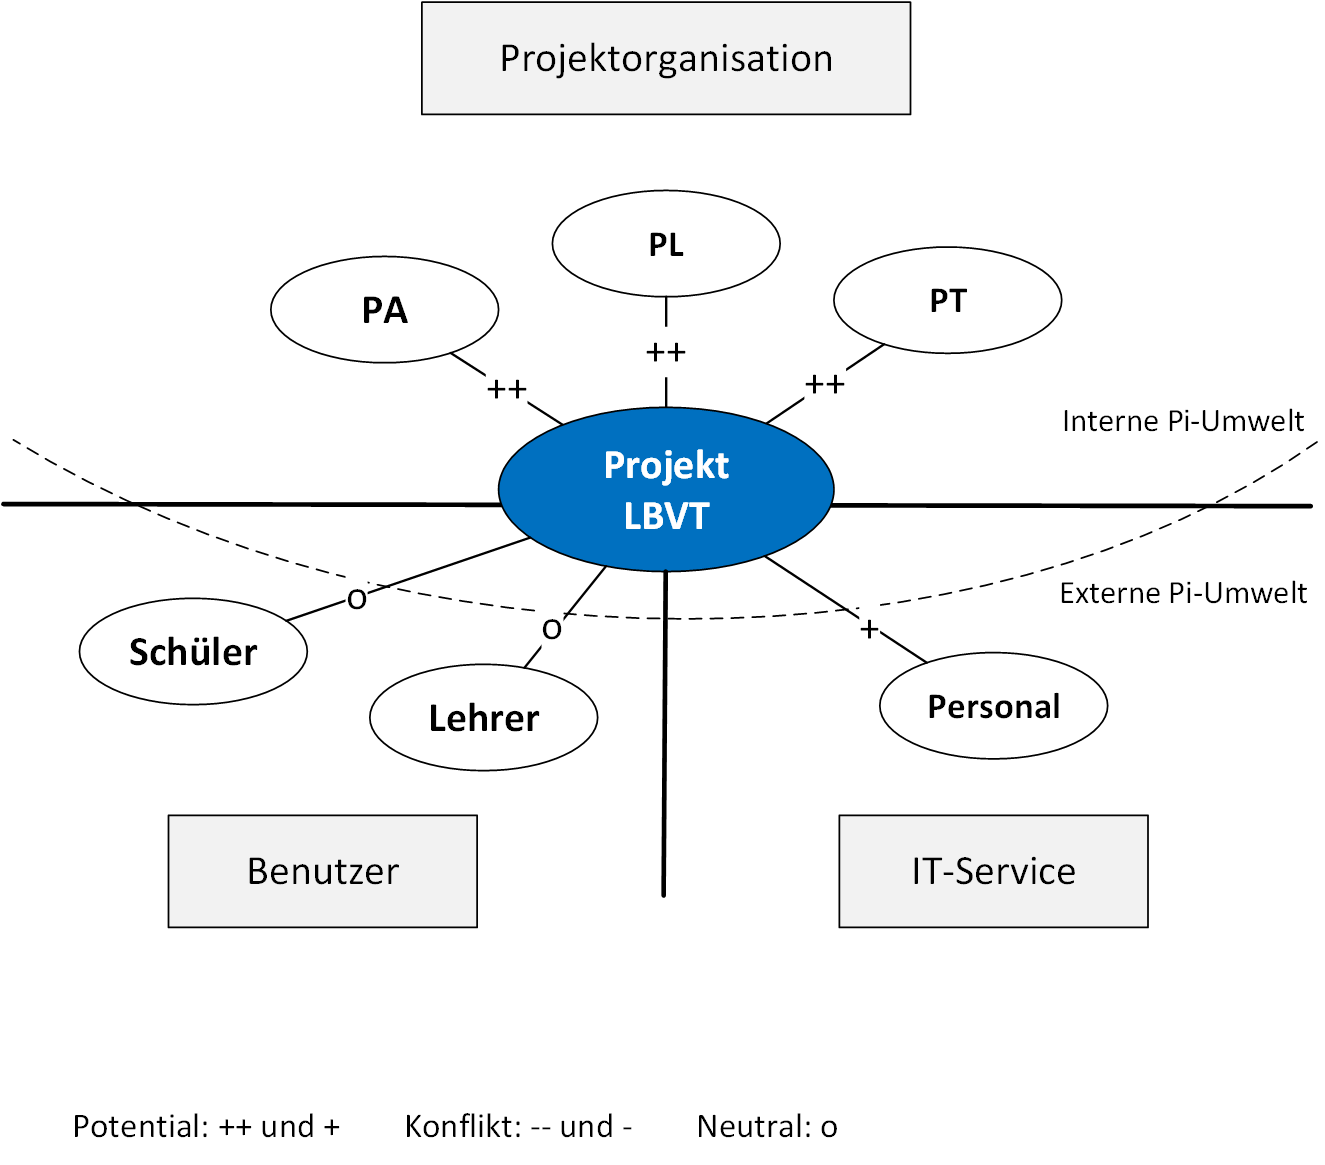
\includegraphics[width=0.8\textwidth]{images/Projektumwelt.png}
    \end{center} \\
    \hline
\end{tabularx}
\endgroup



\begingroup
\begin{scriptsize}
\renewcommand*{\arraystretch}{1.1} % Abstand zwischen Zeilen
\begin{center}
\begin{tabularx}{\textwidth}{|l|p{5.5cm}|X|p{1.8cm}|}
    \hline
    \multicolumn{4}{|c|}{\vspace{-0.005cm}\rowcolor{gray}} \\
    \multicolumn{4}{|c|}{\rowcolor{gray} \bfseries \color{white} \normalsize PROJEKTUMWELTEN-BEZIEHUNGEN \vspace{-0.05cm}} \\
    \multicolumn{4}{|c|}{\rowcolor{gray}} \\
    \hline
    \small \textbf{Umwelten} & \small \textbf{Beziehung} & \small \textbf{Maßnahmen} & \small \textbf{Wer / Wann} \\
    & \scriptsize{(Potential/Konflikt)} & & \scriptsize{\textbf{PSP Code}}\\
    \hline
    PA, PL, PT & ++ & Gemeinsame Planung vom Projekt an einem ruhigen Ort mit Brainstorming. Gemeinsame Auswahl der besten Ideen. & [201],\:[202], [203], [204]\\
    \hline
    IT-Service & + (Es ist gut möglich, dass das IT-Service in Zukunft die Kartenleser teilweise konfigurieren bzw. warten muss, also sollte die Entwicklung des \gls{lbvt} in Kooperation mit Ihnen entstehen. Außerdem besitzen Sie wichtiges Fachwissen über das Schulnetz, was die Projektdurchführung beschleunigen kann.) &
    Gemeinsame Beratung und Alternativensuche mit dem IT-Service. Vorschläge abwiegen und die benutzerfreundlichste und am wenigstens wartungsintensive auswählen. & [201],\:[202], [203],\:[204], [205] \\
    \hline
    Benutzer & o (Ein gut umgesetztes System stimmt Lehrer und Schüler positiv auf die Anwesenheitskontrolle per Kartenleser ein, eine schlechte Umsetzung kann aber Frust und Ignoranz auslösen.) & Gemeinsam mit einzelnen Lehrern und Schülern das System testen und Feedback umsetzen.
umsetzen & [301],\:[304], [402] \\
    \hline
\end{tabularx}
\end{center}
\end{scriptsize}
\endgroup

\newpage
\begin{comment}


\subsection{Beziehungen zu anderen Projekten und Zusammenhang mit den Unternehmenszielen (sachlicher Kontext)}

\begingroup
\renewcommand*{\arraystretch}{1.1} % Abstand zwischen Zeilen
\begin{center}
\begin{tabularx}{\textwidth}{|X|X|p{5.5cm}|X|}
    \hline
    \multicolumn{4}{|c|}{} \\
    \multicolumn{4}{|c|}{\bfseries BEZIEHUNGEN ZU ANDEREN PROJEKTEN} \\
    \multicolumn{4}{|c|}{} \\
    \hline
    \textbf{Programme/} & \textbf{Beziehung} & \textbf{Maßnahmen} & \textbf{Wer / Wann} \\
    \textbf{Projekte/} & \scriptsize{(Potential/Konflikt)} & & \\
    \textbf{Kleinprojekte} & & & \textbf{PSP Code} \\
    \hline
    & & & \\
    \hline
    & & & \\
    \hline
    & & & \\
    \hline
    & & & \\
    \hline
    & & & \\
    \hline
\end{tabularx}
\end{center}
\endgroup

\vspace{0.1cm}

\begingroup
\renewcommand*{\arraystretch}{1.1} % Abstand zwischen Zeilen
\begin{center}
\begin{tabularx}{\textwidth}{|p{3.5cm}|X|}
    \hline
    \multicolumn{2}{|c|}{} \\
    \multicolumn{2}{|c|}{\bfseries ZUSAMMENHANG ZU DEN UNTERNEHMENSZIELEN} \\
    \multicolumn{2}{|c|}{} \\
    \hline
    \textbf{Unternehmensziele} & \textbf{Beschreibung des Zusammenhangs} \\
    \hline
    & \\
    \hline
    & \\
    \hline
    & \\
    \hline
    & \\
    \hline
\end{tabularx}
\end{center}
\endgroup

\newpage
\end{comment}

\subsection{Projektorganigramm}
\vspace{2cm}
\begin{center}
    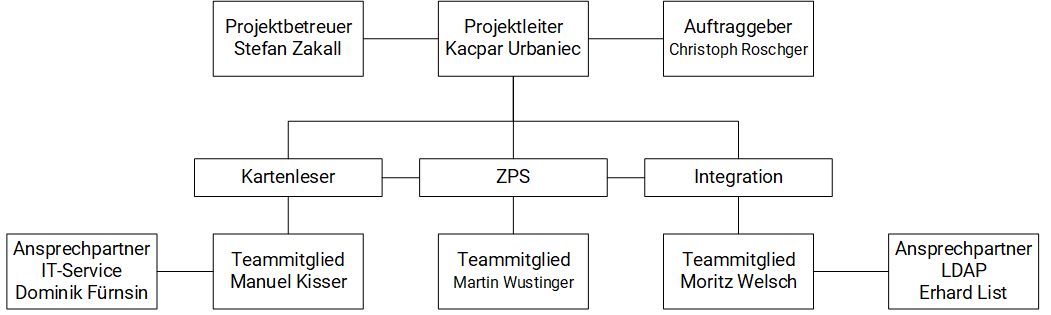
\includegraphics[width=1\textwidth]{images/Organigramm.png}
\end{center}
\vspace{2cm}


\begin{comment}


\begingroup
\renewcommand*{\arraystretch}{1.1} % Abstand zwischen Zeilen
\begin{center}
\begin{tabularx}{\textwidth}{|p{3.2cm}|X|X|}
    \hline
    \multicolumn{3}{|c|}{\vspace{-0.005cm} \rowcolor{gray}} \\
    \multicolumn{3}{|c|}{\rowcolor{gray} \bfseries \color{white} PROJEKTORGANISATION \vspace{-0.05cm}} \\
    \multicolumn{3}{|c|}{\rowcolor{gray}} \\
    \hline
    \textbf{Projektrolle} & \textbf{Aufgabenbereiche/Skills} &  \textbf{Name}\\
    \hline
    \footnotesize ProjektauftraggeberIn & &\\
    \hline
    \footnotesize ProjektleiterIn & &\\
    \hline
    \footnotesize Projektteammitglieder & &\\
    \hline
    \footnotesize ProjektmitarbeiterInnen& &\\
    \hline
\end{tabularx}
\end{center}
\endgroup

\end{comment}

\newpage

\begin{comment}
\subsection{Betrachtungsobjekteplan}

\begingroup
\renewcommand*{\arraystretch}{1.1} % Abstand zwischen Zeilen
\begin{center}
\begin{tabularx}{\textwidth}{|X|}
    \hline
    \multicolumn{1}{|c|}{\vspace{-0.005cm} \rowcolor{gray}} \\
    \multicolumn{1}{|c|}{\rowcolor{gray} \bfseries	\color{white} Betrachtungsobjekteplan \vspace{-0.05cm}} \\
    \multicolumn{1}{|c|}{\rowcolor{gray}} \\
    \hline
    \\
    \hline
\end{tabularx}
\end{center}
\endgroup

\newpage
\end{comment}

% Martin Wustinger
\subsection{Projektstrukturplan} 
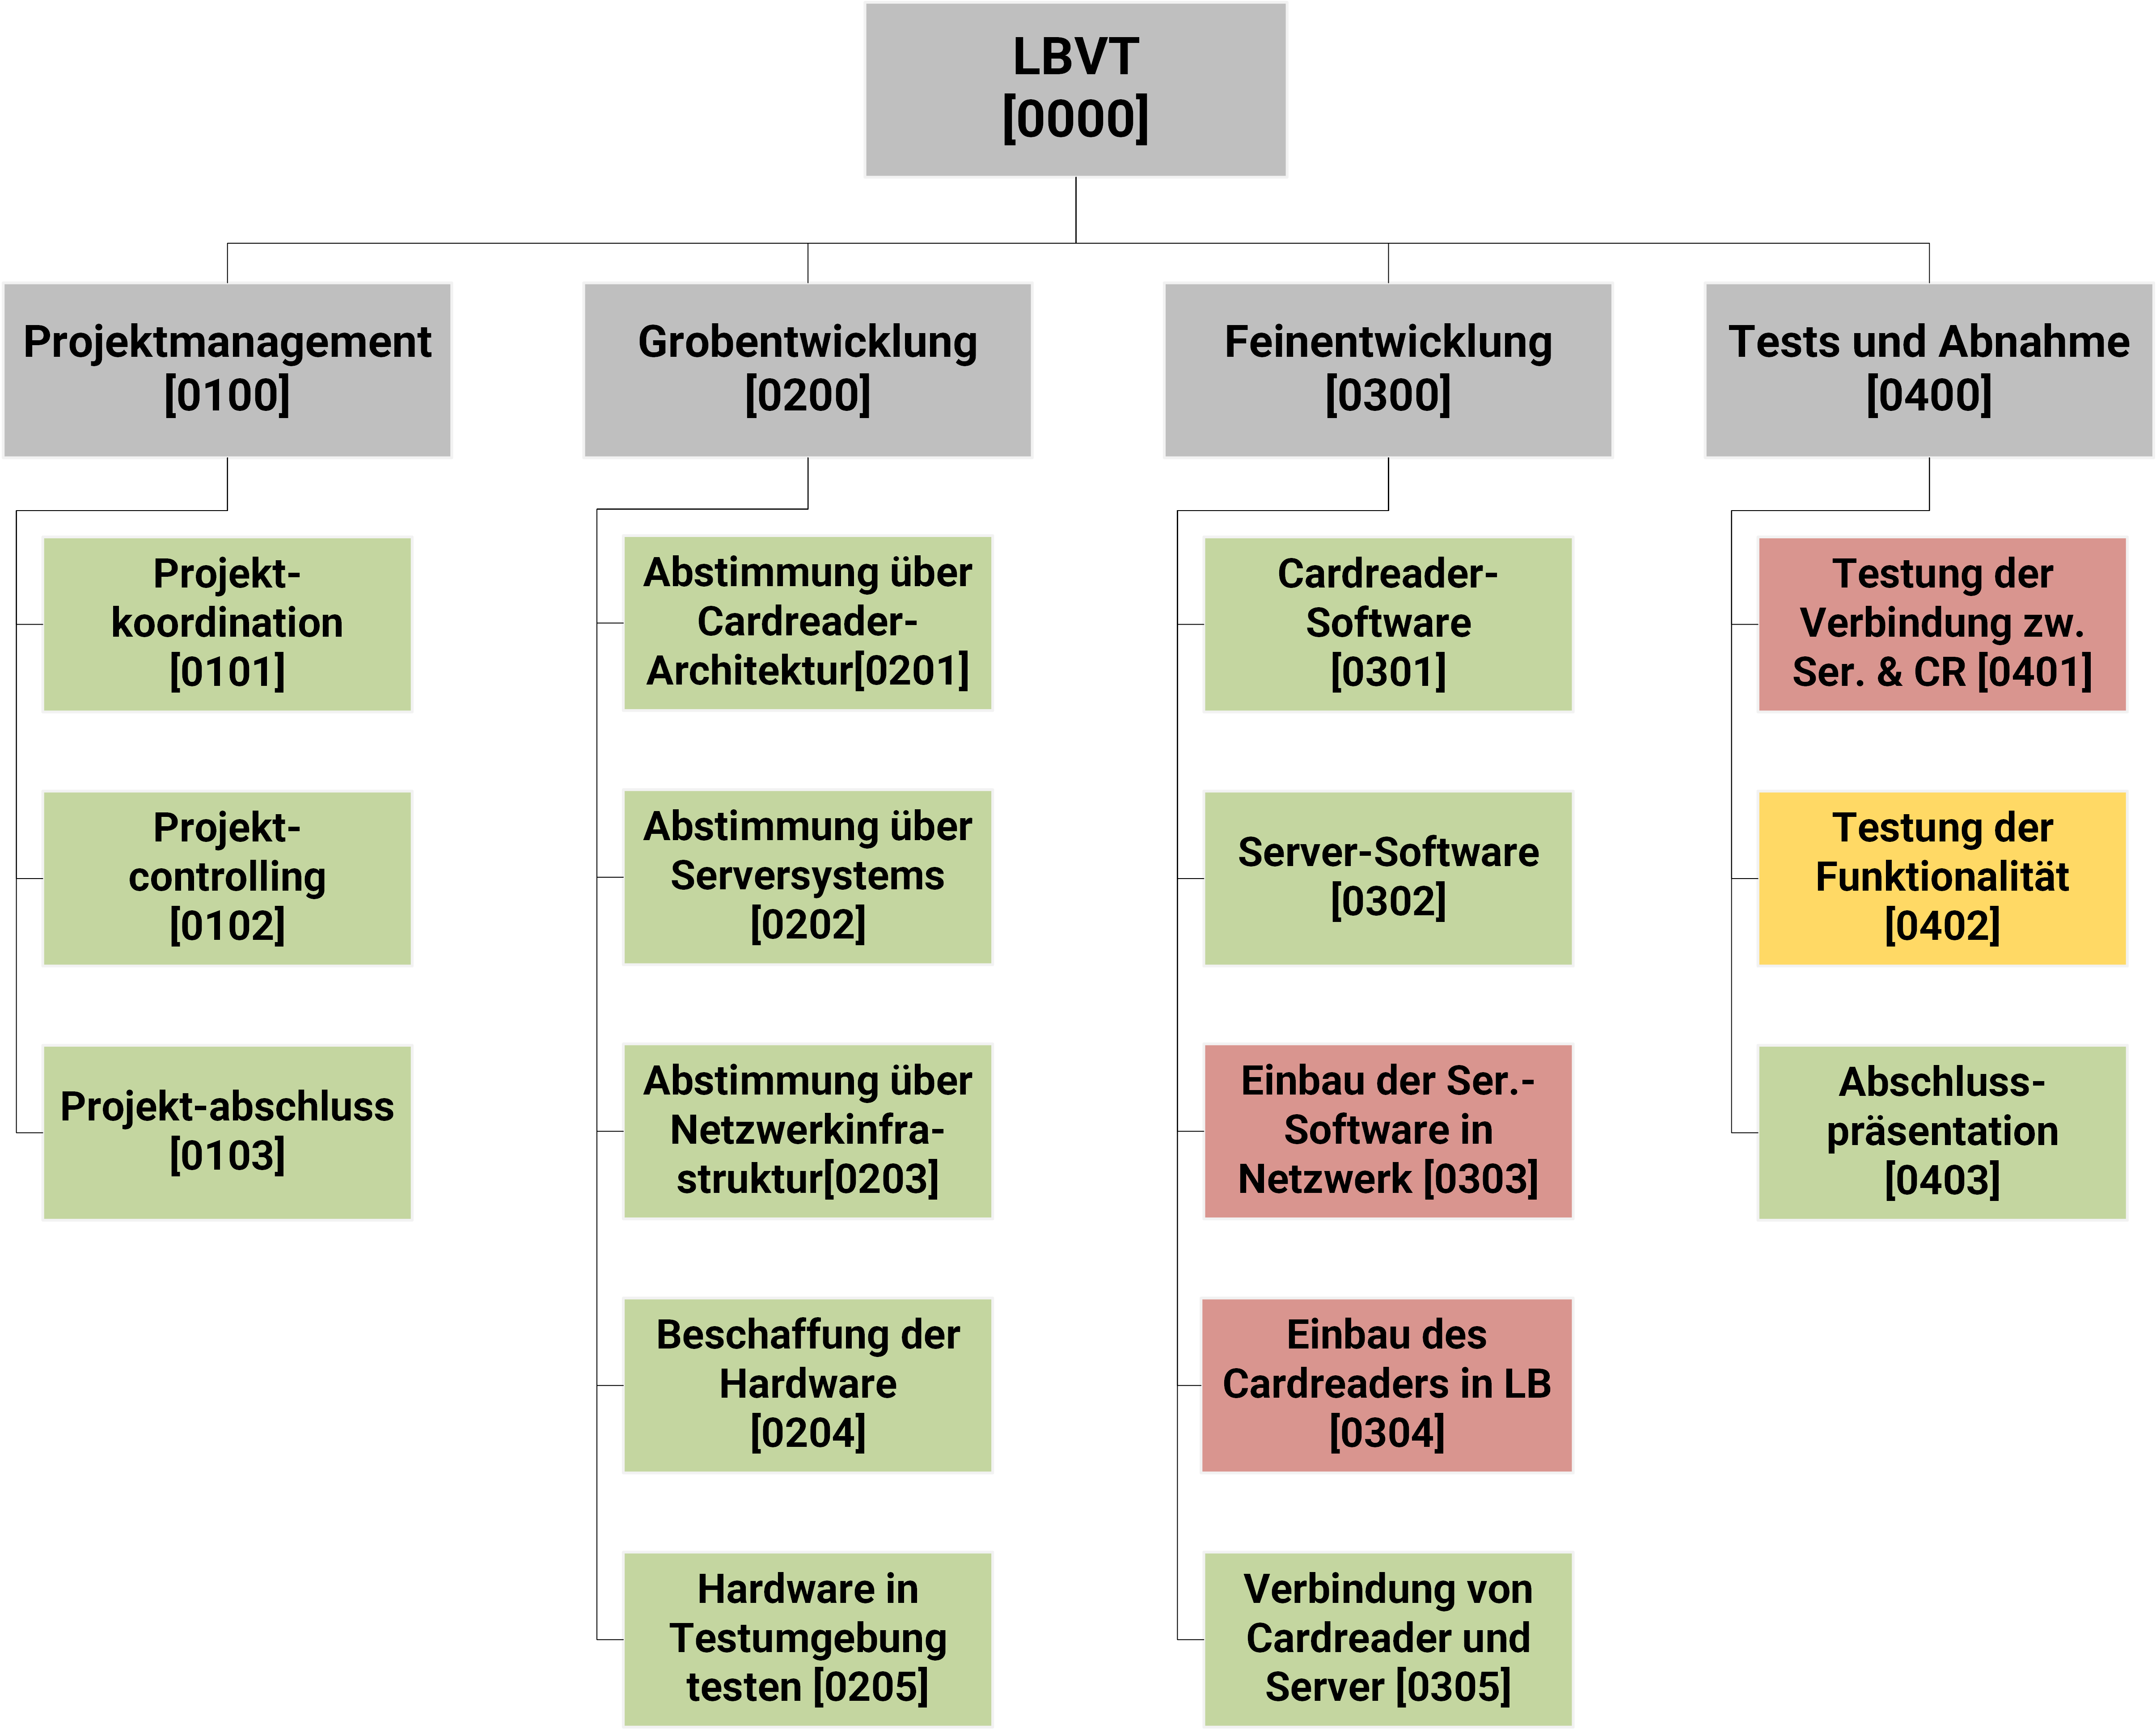
\includegraphics[width=\textwidth]{images/PSP/PSP14.png}

\newpage 


\subsection{Arbeitspaket-Spezifikationen}

% Kacper 101
\begin{scriptsize}
\begingroup
\renewcommand*{\arraystretch}{1.2} % Abstand zwischen Zeilen
\begin{center}
\begin{tabularx}{\textwidth}{|p{2.2cm}|X|}
    \hline
    \multicolumn{2}{|c|}{\vspace{-0.005cm} \rowcolor{gray}} \\
    \multicolumn{2}{|c|}{\rowcolor{gray} \bfseries	\normalsize \color{white} Arbeitspaket-Spezifikationen \vspace{-0.05cm}} \\
    \multicolumn{2}{|c|}{\rowcolor{gray}} \\
    \hline
    \multirow{3}{*}{\shortstack[l]{\textbf{[0101]} \\ \textbf{Projekt-} \\ \textbf{koordination}}} & \textbf{AP-Inhalt} \\
    & \multirow{6}{*}{
    \begin{minipage}{.78\textwidth} 
    \begin{flushleft}
        \begin{itemize} \vspace{-0.6cm} 
         \item Einteilung der Arbeitspakete auf einzelne Teammitglieder
         \item Ausarbeitung aller Dokumente
        \item Absprache des \gls{git}-Workflows
        \item Einhalten des Development-Workflows
    \end{itemize}
    \end{flushleft}
    \end{minipage}} \\
    & & & \\
    & & & \\
    \cline{2-2}
    & \textbf{AP-Nicht-Inhalte} \\
    & %\multirow{6}{*}{
    %\begin{minipage}{.78\textwidth} 
    %\begin{flushleft}
    %    \begin{itemize} \vspace{-0.6cm}  
    %     \item Beschaffung der Hardware
    %     \item Zusammenbau der Hardware
    %     \item Inbetriebnahme der Hardware
    %     \item \text{}
    %     \item \text{}
    %\end{itemize}
    %\end{flushleft}
    %\end{minipage}} 
    \\
    %& & & \\
    %& & & \\
     \cline{2-2}
    & \textbf{AP-Ergebnis} \\
    & \multirow{7}{*}{
    \begin{minipage}{.78\textwidth} 
    \begin{flushleft}
        \begin{itemize} \vspace{-0.1cm} 
         \item Teile der Arbeitspakete wurden nach besten Kenntnissen auf einzelne Teammitglieder verteilt
        \item Alle Dokumente (Projektantrag, Lastenheft, Machbarkeitsstudie, Pflichtenheft) sind fertig gestellt
        \item \gls{git}-Workflow wurde abgesprochen und während der Projektdauer eingehalten
        \item Development-Workflow wurde abgesprochen und während der Projektdauer eingehalten
    \end{itemize}
    \end{flushleft}
    \end{minipage}} \\
    & & & \\
    & & & \\& & & \\
     \cline{2-2}
    & \textbf{AP-Leistungsfortschrittmessung} \\
    & \multirow{8}{*}{
    \begin{minipage}{.78\textwidth} 
    \begin{flushleft}
        \begin{itemize}[leftmargin=7mm] \vspace{-0.4cm}  
        \item[10\%] Aufteilung der Arbeitspakete auf Teammitglieder, Erstellung eines Projektorganigramms und Beginn der Zeitaufzeichnung
        \item[60\%] Fertigstellung und Abgabe aller Dokumente
        \item[80\%] Überprüfung der \gls{git}-Repository History, um die Einhaltung des Workflows zu gewährleisten
        \item[100\%] Überprüfung von Hardware und Code, schauen ob Hardware Spezifikationen erfüllt, korrekt aufgebaut ist und kontrollieren ob alle Programme eine Dokumentation bieten
         %\item Projektorganigramm, Zeitaufzeichnung
         %\item \gls{git}-Repository History überprüfen
         %\item Abgabe der Dokumente (bisher Projektantrag, Lastenheft)
    \end{itemize}
    \end{flushleft}
    \end{minipage}} \\
    & & & \\
    & & & \\
    & & & \\
    
    \hline
\end{tabularx}
\end{center}
\endgroup
\end{scriptsize}
\newpage

% Kacper 102
\begin{scriptsize}
\begingroup
\renewcommand*{\arraystretch}{1.2} % Abstand zwischen Zeilen
\begin{center}
\begin{tabularx}{\textwidth}{|p{2.2cm}|X|}
    \hline
    \multicolumn{2}{|c|}{\vspace{-0.005cm} \rowcolor{gray}} \\
    \multicolumn{2}{|c|}{\rowcolor{gray} \bfseries	\normalsize \color{white} Arbeitspaket-Spezifikationen \vspace{-0.05cm}} \\
    \multicolumn{2}{|c|}{\rowcolor{gray}} \\
    \hline
    \multirow{2}{*}{\shortstack[l]{\textbf{[0102]} \\ \textbf{Projektcontrolling
} }} & \textbf{AP-Inhalt} \\
    & \multirow{6}{*}{
    \begin{minipage}{.78\textwidth} 
    \begin{flushleft}
        \begin{itemize} \vspace{-0.6cm} 
         \item Fortschrittskontrolle bei Projektteammitgliedern
        \item Klärung von Ungereimtheiten bei Anforderungen des Lasten-/Pflichtenhefts
        \item Überprüfung von Einhaltung der Arbeitsanforderungen
    \end{itemize}
    \end{flushleft}
    \end{minipage}} \\
    & & & \\
    & & & \\
    \cline{2-2}
    & \textbf{AP-Nicht-Inhalte} \\
    & \multirow{6}{*}{
    \begin{minipage}{.78\textwidth} 
    \begin{flushleft}
        \begin{itemize} \vspace{-0.6cm}  
         \item Überprüfung der Validität von Programmen
         \item Allgemeine Hardware-Inspektionen 
        \item Überprüfung der Performance der Hardware in Kombination mit Software
    \end{itemize}
    \end{flushleft}
    \end{minipage}} \\
    & & & \\
    & & & \\
     \cline{2-2}
    & \textbf{AP-Ergebnis} \\
    & \multirow{6}{*}{
    \begin{minipage}{.78\textwidth} 
    \begin{flushleft}
        \begin{itemize} \vspace{-0.6cm} 
         \item Fortschrittskontrolle durch Projektleiter
         \item Alle aufgetretenen Ungereimtheiten wurden gelöst
         \item Einhaltung der Arbeitsanforderungen wurde durchgeführt
    \end{itemize}
    \end{flushleft}
    \end{minipage}} \\
    & & & \\
    & & & \\
     \cline{2-2}
    & \textbf{AP-Leistungsfortschrittmessung} \\
    & \multirow{6}{*}{
    \begin{minipage}{.78\textwidth} 
    \begin{flushleft}
        \begin{itemize}[leftmargin=7mm] \vspace{-0.6cm}  
         \item[100\%] Regelmäßige Kontrolle der Zeitaufzeichnung als Mittel zur Sicherung der Fortschrittskontrolle
         \item[100\%] Regelmäßgie Begutachtung, ob Arbeitspakete  zeitgerecht fertiggestellt werden
         \item[100\%] Überprüfung aller Statusberichte
    \end{itemize}
    \end{flushleft}
    \end{minipage}} \\
    & & & \\
    & & & \\
    \hline
\end{tabularx}
\end{center}
\endgroup
\end{scriptsize}
\newpage

% Kacper 103
\begin{scriptsize}
\begingroup
\renewcommand*{\arraystretch}{1.2} % Abstand zwischen Zeilen
\begin{center}
\begin{tabularx}{\textwidth}{|p{2.2cm}|X|}
    \hline
    \multicolumn{2}{|c|}{\vspace{-0.005cm} \rowcolor{gray}} \\
    \multicolumn{2}{|c|}{\rowcolor{gray} \bfseries	\normalsize \color{white} Arbeitspaket-Spezifikationen \vspace{-0.05cm}} \\
    \multicolumn{2}{|c|}{\rowcolor{gray}} \\
    \hline
    \multirow{2}{*}{\shortstack[l]{\textbf{[0103]} \\ \textbf{Projekt-} \\ \textbf{abschluss}}} & \textbf{AP-Inhalt} \\
    & \multirow{6}{*}{
    \begin{minipage}{.78\textwidth} 
    \begin{flushleft}
        \begin{itemize} \vspace{-1.6cm} 
         \item \gls{lbvt} wird entsprechend des Vertragsgegenstandes fertiggestellt
    \end{itemize}
    \end{flushleft}
    \end{minipage}} \\
    & & & \\
    \cline{2-2}
    & \textbf{AP-Nicht-Inhalte} \\
    & \multirow{2}{*}{
    \begin{minipage}{.78\textwidth} 
    \begin{flushleft}
        \begin{itemize} %\vspace{-1.0cm}  
         \item Erbringen von Produkt-Leistungen, die nicht im Vertragsgegenstand festgelegt wurden
    \end{itemize}
    \end{flushleft}
    \end{minipage}} \\
    & & & \\
     \cline{2-2}
    & \textbf{AP-Ergebnis} \\
    & \multirow{6}{*}{
    \begin{minipage}{.78\textwidth} 
    \begin{flushleft}
        \begin{itemize} \vspace{-0.6cm} 
         \item Erstellung eines mobilen Kartenlesers als Muster, welcher Schülerkarten einlesen kann
         \item Realisierung eines \gls{zps} als Bindeglied zwischen Kartenleser und \gls{lba}
         \item Erstellung einer grafischen Oberfläche für die Kartenleserverwaltung in der \gls{lba} 
         \item Umgesetztes Sicherheitskonzept für das \gls{lbvt}
    \end{itemize}
    \end{flushleft}
    \end{minipage}} \\
    & & & \\
    & & & \\
     \cline{2-2}
    & \textbf{AP-Leistungsfortschrittmessung} \\
    & \multirow{7}{*}{
    \begin{minipage}{.78\textwidth} 
    \begin{flushleft}
        \begin{itemize}[leftmargin=7mm] \vspace{-1.0cm}  
         %\item Fertiggestellte Arbeitspakete
         \item[30\%] Abschluss der Grobentwicklung
         \item[70\%] Abschluss der Feinentwicklung
         \item[100\%] Abschluss der Testung und Abnahme
    \end{itemize}
    \end{flushleft}
    \end{minipage}} \\
    & & & \\   & & & \\

    \hline
\end{tabularx}
\end{center}
\endgroup
\end{scriptsize}
\newpage

%AP 201 von mwustinger 
\begin{scriptsize}
\begingroup
\renewcommand*{\arraystretch}{1.2} % Abstand zwischen Zeilen
\begin{center}
\begin{tabularx}{\textwidth}{|p{2.2cm}|X|}
    \hline
    \multicolumn{2}{|c|}{\vspace{-0.005cm} \rowcolor{gray}} \\
    \multicolumn{2}{|c|}{\rowcolor{gray} \bfseries	\normalsize \color{white} Arbeitspaket-Spezifikationen \vspace{-0.05cm}} \\
    \multicolumn{2}{|c|}{\rowcolor{gray}} \\
    \hline
    \multirow{4}{*}{\shortstack[l]{\textbf{[0201]} \\ \textbf{Abstimmung über} \\ \textbf{Cardreader -} \\ \textbf{Architektur}}} & \textbf{AP-Inhalt} \\
    & \multirow{6}{*}{
    \begin{minipage}{.78\textwidth} 
    \begin{flushleft}
        \begin{itemize} \vspace{-0.6cm} 
         \item Auswahl einer geeigneten Kartenleser Architektur
         \item Bestimmung einer geeigneten Microcontroller-Architektur
         \item Bestimmung eines kompatiblen Kartenlesers
         \item Bestimmung des Software-Aufbaus des Kartenlesers
    \end{itemize}
    \end{flushleft}
    \end{minipage}} \\
    & & & \\
    & & & \\
    \cline{2-2}
    & \textbf{AP-Nicht-Inhalte} \\
    & \multirow{6}{*}{
    \begin{minipage}{.78\textwidth} 
    \begin{flushleft}
        \begin{itemize} \vspace{-0.6cm}  
         \item Beschaffung der Hardware
         \item Zusammenbau der Hardware
         \item Inbetriebnahme der Hardware
    \end{itemize}
    \end{flushleft}
    \end{minipage}} \\
    & & & \\
    & & & \\
     \cline{2-2}
    & \textbf{AP-Ergebnis} \\
    & \multirow{6}{*}{
    \begin{minipage}{.78\textwidth} 
    \begin{flushleft}
        \begin{itemize} \vspace{-0.6cm} 
         \item Eine Kartenleser Architektur wurde bestimmt (Raspberry PI)
         \item Ein dafür geeigneter Kartenleser mit vorhandenen Libraries ist herrausgesucht
         \item Ein Software Grobkonzept wie die Zusammenarbeit der Scripte realisiert wird, wurde erarbeitet
    \end{itemize}
    \end{flushleft}
    \end{minipage}} \\
    & & & \\
    & & & \\
     \cline{2-2}
    & \textbf{AP-Leistungsfortschrittmessung} \\
    & \multirow{6}{*}{
    \begin{minipage}{.78\textwidth} 
    \begin{flushleft}
        \begin{itemize} [leftmargin=7mm] \vspace{-0.6cm}  
         \item [40\%] Kartenleser Architektur wurde festgelegt
         \item [70\%] Dafür geeignetes Kartenlesermodul wurde bestimmt
         \item [100\%] Grobkonzept der Software wurde erstellt
    \end{itemize}
    \end{flushleft}
    \end{minipage}} \\
    & & & \\
    & & & \\
    \hline
\end{tabularx}
\end{center}
\endgroup
\end{scriptsize}
\newpage

%AP 202 von mwustinger 
\begin{scriptsize}
\begingroup
\renewcommand*{\arraystretch}{1.2} % Abstand zwischen Zeilen
\begin{center}
\begin{tabularx}{\textwidth}{|p{2.2cm}|X|}
    \hline
    \multicolumn{2}{|c|}{\vspace{-0.005cm} \rowcolor{gray}} \\
    \multicolumn{2}{|c|}{\rowcolor{gray} \bfseries	\normalsize \color{white} Arbeitspaket-Spezifikationen \vspace{-0.05cm}} \\
    \multicolumn{2}{|c|}{\rowcolor{gray}} \\
    \hline
    \multirow{4}{*}{\shortstack[l]{\textbf{[0202]} \\ \textbf{Abstimmung über} \\ \textbf{Serversystem -} \\ \textbf{Architektur}}} & \textbf{AP-Inhalt} \\
    & \multirow{6}{*}{
    \begin{minipage}{.78\textwidth} 
    \begin{flushleft}
        \begin{itemize} \vspace{-0.6cm} 
         \item Auswahl einer geeigneten Serversystem Architektur
         \item Bestimmung eines geeigneten Server-Betriebsystem
         \item Bestimmung eines geeigneten Datenbanksystem
         \item Bestimmung des Software-Aufbaus des Servers
    \end{itemize}
    \end{flushleft}
    \end{minipage}} \\
    & & & \\
    & & & \\
    \cline{2-2}
    & \textbf{AP-Nicht-Inhalte} \\
    & \multirow{6}{*}{
    \begin{minipage}{.78\textwidth} 
    \begin{flushleft}
        \begin{itemize} \vspace{-0.6cm}  
         \item Beschaffung einer  Server-Hardware
         \item Programmierung von Scripten, welche auf dem Server laufen
         \item Programmierung der Datenbank
    \end{itemize}
    \end{flushleft}
    \end{minipage}} \\
    & & & \\
    & & & \\
     \cline{2-2}
    & \textbf{AP-Ergebnis} \\
    & \multirow{6}{*}{
    \begin{minipage}{.78\textwidth} 
    \begin{flushleft}
        \begin{itemize} \vspace{-0.6cm} 
         \item Eine Server Architektur wurde bestimmt (Ubuntu Server)
         \item Ein Datenbank System wurde bestimmt (MariaDB)
         \item Ein Software Grobkonzept wie die Zusammenarbeit der Scripte realisiert wird, wurde erarbeitet
    \end{itemize}
    \end{flushleft}
    \end{minipage}} \\
    & & & \\
    & & & \\
     \cline{2-2}
    & \textbf{AP-Leistungsfortschrittmessung} \\
    & \multirow{6}{*}{
    \begin{minipage}{.78\textwidth} 
    \begin{flushleft}
        \begin{itemize} [leftmargin=7mm] \vspace{-0.6cm}  
         \item [25\%] Server Architektur wurde festgelegt
         \item [50\%] Datenbank System wurde festgelegt
         \item [100\%] Grobkonzept der Software wurde erstellt
    \end{itemize}
    \end{flushleft}
    \end{minipage}} \\
    & & & \\
    & & & \\
    \hline
\end{tabularx}
\end{center}
\endgroup
\end{scriptsize}
\newpage

%AP 203 von mkisser
\begin{scriptsize}
\begingroup
\renewcommand*{\arraystretch}{1.2} % Abstand zwischen Zeilen
\begin{center}
\begin{tabularx}{\textwidth}{|p{2.2cm}|X|}
    \hline
    \multicolumn{2}{|c|}{\vspace{-0.005cm} \rowcolor{gray}} \\
    \multicolumn{2}{|c|}{\rowcolor{gray} \bfseries	\normalsize \color{white} Arbeitspaket-Spezifikationen \vspace{-0.05cm}} \\
    \multicolumn{2}{|c|}{\rowcolor{gray}} \\
    \hline
    \multirow{4}{*}{\shortstack[l]{\textbf{[0203]} \\ \textbf{Abstimmung über} \\ \textbf{Netzwerkinfra-} \\ \textbf{struktur}}} & \textbf{AP-Inhalt} \\
    & \multirow{6}{*}{
    \begin{minipage}{.78\textwidth} 
    \begin{flushleft}
        \begin{itemize} \vspace{-0.6cm} 
         \item Bestimmung der Einbindungsart in vorhandenes Netzwerk
         \item Abstimmung mit IT-Service über Einbindungsart
         \item Erstellung eines Plans zur Implementierung
    \end{itemize}
    \end{flushleft}
    \end{minipage}} \\
    & & & \\
    & & & \\
    \cline{2-2}
    & \textbf{AP-Nicht-Inhalte} \\
    & \multirow{6}{*}{
    \begin{minipage}{.78\textwidth} 
    \begin{flushleft}
        \begin{itemize} \vspace{-0.6cm}  
         \item Implementierung des Systems im bestehenden Netzwerk
         \item Abänderung des bestehenden Systems
    \end{itemize}
    \end{flushleft}
    \end{minipage}} \\
    & & & \\
    & & & \\
     \cline{2-2}
    & \textbf{AP-Ergebnis} \\
    & \multirow{6}{*}{
    \begin{minipage}{.78\textwidth} 
    \begin{flushleft}
        \begin{itemize} \vspace{-0.6cm} 
         \item Strategie zur Einbindung der Kartenlesegeräte in das vorhandene Netzwerk
         \item Strategie zur Einbindung des \gls{zps} in das vorhandene Netzwerk
    \end{itemize}
    \end{flushleft}
    \end{minipage}} \\
    & & & \\
    & & & \\
     \cline{2-2}
    & \textbf{AP-Leistungsfortschrittmessung} \\
    & \multirow{6}{*}{
    \begin{minipage}{.78\textwidth} 
    \begin{flushleft}
        \begin{itemize}[leftmargin=7mm] \vspace{-1.0cm}
         \item[15\%] Möglichkeiten zur Einbindung in vorhandenem Netzwerk konkretisiert
         \item[50\%] Netzwerkspezifikationen vom IT-Service bekommen
         \item[100\%] Plan zur Implementierung in bestehendes Netzwerk fertiggestellt
    \end{itemize}
    \end{flushleft}
    \end{minipage}} \\
    & & & \\
    & & & \\
    \hline
\end{tabularx}
\end{center}
\endgroup
\end{scriptsize}
\newpage

%AP 204 von mkisser
\begin{scriptsize}
\begingroup
\renewcommand*{\arraystretch}{1.2} % Abstand zwischen Zeilen
\begin{center}
\begin{tabularx}{\textwidth}{|p{2.2cm}|X|}
    \hline
    \multicolumn{2}{|c|}{\vspace{-0.005cm} \rowcolor{gray}} \\
    \multicolumn{2}{|c|}{\rowcolor{gray} \bfseries	\normalsize \color{white} Arbeitspaket-Spezifikationen \vspace{-0.05cm}} \\
    \multicolumn{2}{|c|}{\rowcolor{gray}} \\
    \hline
    \multirow{4}{*}{\shortstack[l]{\textbf{[0204]} \\ \textbf{Beschaffung der} \\ \textbf{Hardware}}} & \textbf{AP-Inhalt} \\
    & \multirow{6}{*}{
    \begin{minipage}{.78\textwidth} 
    \begin{flushleft}
        \begin{itemize} \vspace{-0.6cm} 
         \item Benötigte Hardware bestellen
         \item Benötigte Hardware auf Funktionalität prüfen
         \item Hardware für Variantenbildung bestellen
    \end{itemize}
    \end{flushleft}
    \end{minipage}} \\
    & & & \\
    & & & \\
    \cline{2-2}
    & \textbf{AP-Nicht-Inhalte} \\
    & \multirow{6}{*}{
    \begin{minipage}{.78\textwidth} 
    \begin{flushleft}
        \begin{itemize} \vspace{-0.6cm}  
         \item Bestimmung der benötigten Hardware
    \end{itemize}
    \end{flushleft}
    \end{minipage}} \\
    & & & \\
    & & & \\
     \cline{2-2}
    & \textbf{AP-Ergebnis} \\
    & \multirow{6}{*}{
    \begin{minipage}{.78\textwidth} 
    \begin{flushleft}
        \begin{itemize} \vspace{-0.6cm} 
         \item Vorhandensein der benötigten Hardware zur Entwicklung eines Kartenlesers
         \item Vorhandensein der benötigten Hardware zur Entwicklung von Varianten des Kartenlesers
    \end{itemize}
    \end{flushleft}
    \end{minipage}} \\
    & & & \\
    & & & \\
     \cline{2-2}
    & \textbf{AP-Leistungsfortschrittmessung} \\
    & \multirow{6}{*}{
    \begin{minipage}{.78\textwidth} 
    \begin{flushleft}
        \begin{itemize}[leftmargin=7mm] \vspace{-0.6cm} 
         \item[20\%] Benötigte Hardware bestellt
         \item[40\%] Benötigte Hardware geliefert
         \item[60\%] Benötigte Hardware in einwandfreiem Zustand
         \item[80\%] Benötigte Hardware zur Variantenbildung bestellt
         \item[100\%] Benötigte Hardware zur Variantenbildung geliefert
    \end{itemize}
    \end{flushleft}
    \end{minipage}} \\
    & & & \\
    & & & \\
    \hline
\end{tabularx}
\end{center}
\endgroup
\end{scriptsize}
\newpage

%AP 205 von mwelsch
\begin{scriptsize}
\begingroup
\renewcommand*{\arraystretch}{1.2} % Abstand zwischen Zeilen
\begin{center}
\begin{tabularx}{\textwidth}{|p{2.2cm}|X|}
    \hline
    \multicolumn{2}{|c|}{\vspace{-0.005cm} \rowcolor{gray}} \\
    \multicolumn{2}{|c|}{\rowcolor{gray} \bfseries	\normalsize \color{white} Arbeitspaket-Spezifikationen \vspace{-0.05cm}} \\
    \multicolumn{2}{|c|}{\rowcolor{gray}} \\
    \hline
    \multirow{4}{*}{\shortstack[l]{\textbf{[0205]} \\ \textbf{Hardware in} \\ \textbf{Testumgebung} \\ \textbf{einsetzen}}} & \textbf{AP-Inhalt} \\
    & \multirow{6}{*}{
    \begin{minipage}{.78\textwidth} 
    \begin{flushleft}
        \begin{itemize} \vspace{-0.6cm} 
         \item Aufbau des Kartenlesers mit der ausgewählten Hardware
         \item Kartenleser in Netzwerk einbinden
         \item Netzwerk verbindung ausführlich testen
         \item Ein Script programmieren welches die ID der Educard ausließt
    \end{itemize}
    \end{flushleft}
    \end{minipage}} \\
    & & & \\
    & & & \\
    \cline{2-2}
    & \textbf{AP-Nicht-Inhalte} \\
    & \multirow{6}{*}{
    \begin{minipage}{.78\textwidth} 
    \begin{flushleft}
        \begin{itemize} \vspace{-0.6cm}  
         \item Beschaffung jeglicher Hardware
         \item Entwickeln einer Kartenleser-Software welche mehrere Karten erkennt, diese speichert oder diese weitersendet
         \item Entwickeln der Server-Software
    \end{itemize}
    \end{flushleft}
    \end{minipage}} \\
    & & & \\
    & & & \\
     \cline{2-2}
    & \textbf{AP-Ergebnis} \\
    & \multirow{6}{*}{
    \begin{minipage}{.78\textwidth} 
    \begin{flushleft}
        \begin{itemize} \vspace{-0.6cm} 
         \item Ein Script zur Auslesung der ID einer Educard ist verfügbar
         \item Der Kartenleser besitzt eine bestehende Verbindung zum Internet
    \end{itemize}
    \end{flushleft}
    \end{minipage}} \\
    & & & \\
    & & & \\
     \cline{2-2}
    & \textbf{AP-Leistungsfortschrittmessung} \\
    & \multirow{6}{*}{
    \begin{minipage}{.78\textwidth} 
    \begin{flushleft}
        \begin{itemize}[leftmargin=7mm] \vspace{-0.6cm} 
         \item[25\%] Der Kartenleser wurde mit der ausgewählten Hardware aufgebaut
         \item[50\%] Der Kartenleser wurde im Netzwerk eingebunden
         \item[100\%] Ein Script kann die ID der Educards auslesen
    \end{itemize}
    \end{flushleft}
    \end{minipage}} \\
    & & & \\
    & & & \\
    \hline
\end{tabularx}
\end{center}
\endgroup
\end{scriptsize}
\newpage
%ende AP 205


%AP 301
\begin{scriptsize}
\begingroup
\renewcommand*{\arraystretch}{1.2} % Abstand zwischen Zeilen
\begin{center}
\begin{tabularx}{\textwidth}{|p{2.2cm}|X|}
    \hline
    \multicolumn{2}{|c|}{\vspace{-0.005cm} \rowcolor{gray}} \\
    \multicolumn{2}{|c|}{\rowcolor{gray} \bfseries	\normalsize \color{white} Arbeitspaket-Spezifikationen \vspace{-0.05cm}} \\
    \multicolumn{2}{|c|}{\rowcolor{gray}} \\
    \hline
    \multirow{2}{*}{\shortstack[l]{\textbf{[0301]} \\ \textbf{Cardreader-} \\ \textbf{Software} }} & \textbf{AP-Inhalt} \\
    & \multirow{9}{*}{ % ICH HABE DAS VON 6 AUF 9 GEÄNDERT UND ZEILE 756-758 HINZUGEFÜGT 
    \begin{minipage}{.78\textwidth} 
    \begin{flushleft}
        \begin{itemize} %\vspace{-0.6cm} 
         \item Datenbank am Kartenleser einrichten
         \item Das bereits vorhande Script wartet auf eine Educard und speichert die ID der Educard und das Datum in die Datenbank
         \item Ein Script welches sobald der Datenbank ein Element hinzugefügt wird versucht alle Einträge der Datenbank an den Server zu senden
	 \item Falls das senden erfolgreich war werden alle gesendeten Elemente aus der Datenbank enternt
	 \item Die Scripte geben Feedback ob das einlesen der Karte erfolgreich war und ob eine Verbindung zum Server besteht.
    \end{itemize}
    \end{flushleft}
    \end{minipage}} \\
    & & & \\
    & & & \\
    & & & \\
    & & & \\
  
    \cline{2-2}
    & \textbf{AP-Nicht-Inhalte} \\
    & \multirow{6}{*}{
    \begin{minipage}{.78\textwidth} 
    \begin{flushleft}
        \begin{itemize} \vspace{-0.6cm}  
         \item Netzwerkverbindung zum Server sicherstellen
	 \item Server-Software programmieren
    \end{itemize}
    \end{flushleft}
    \end{minipage}} \\
    & & & \\
    & & & \\
     \cline{2-2}
    & \textbf{AP-Ergebnis} \\
    & \multirow{6}{*}{
    \begin{minipage}{.78\textwidth} 
    \begin{flushleft}
        \begin{itemize} \vspace{-0.6cm} 
         \item Der Server wartet auf eine Educard, liest diese ein, gibt Feedback ob dies erflogreich war und sendet den Datenbankeintrag an den \gls{zps} weiter.
         %\item \text{}
         %\item \text{}
         %\item \text{}
         %\item \text{}
    \end{itemize}
    \end{flushleft}
    \end{minipage}} \\
    & & & \\
    & & & \\
     \cline{2-2}
    & \textbf{AP-Leistungsfortschrittmessung} \\
    & \multirow{6}{*}{
    \begin{minipage}{.78\textwidth} 
    \begin{flushleft}
        \begin{itemize}[leftmargin=7mm] %\vspace{-0.6cm} 
         \item[15\%] Die Datenbank wurde am Kartenleser eingerichtet
         \item[40\%] Ein Script welches Educard-IDs in die Datenbank hinzufügt ist funktionsfähig
         \item[65\%] Dieses Script gibt Feedback ob dies erfolgreich war
         \item[85\%] Ein Script welches die Datenbankeinträge an den \gls{zps} sendet ist funktionsfähig
         \item[100\%] Bei erfolgreichem senden werden die gesendeten Elemente aus der lokalen Datenbank gelöscht
         %\item \text{}
         %\item \text{}
         %\item \text{}
    \end{itemize}
    \end{flushleft}
    \end{minipage}} \\
    & & & \\
    & & & \\
    & & & \\
    \hline
\end{tabularx}
\end{center}
\endgroup
\end{scriptsize}
\newpage
%end AP 301

%AP 302 von mwustinger 
\begin{scriptsize}
\begingroup
\renewcommand*{\arraystretch}{1.2} % Abstand zwischen Zeilen
\begin{center}
\begin{tabularx}{\textwidth}{|p{2.2cm}|X|}
    \hline
    \multicolumn{2}{|c|}{\vspace{-0.005cm} \rowcolor{gray}} \\
    \multicolumn{2}{|c|}{\rowcolor{gray} \bfseries	\normalsize \color{white} Arbeitspaket-Spezifikationen \vspace{-0.05cm}} \\
    \multicolumn{2}{|c|}{\rowcolor{gray}} \\
    \hline
    \multirow{2}{*}{\shortstack[l]{\textbf{[0302]} \\ \textbf{Server-Software}}} & \textbf{AP-Inhalt} \\
    & \multirow{6}{*}{
    \begin{minipage}{.78\textwidth} 
    \begin{flushleft}
        \begin{itemize} \vspace{-0.6cm} 
         \item Input-Script in Python (Ließt gesendete Daten über ZMQ-Schnittstelle aus)
         \item LBA-Script in Python (Schreibt die Daten in die \gls{lba})
         \item Web-Script (Stellt das Webinterface für die Raumzuteilung zur Verfügung)
         \item Datenbank welche die Anwesenheits-Einträge speichert
    \end{itemize}
    \end{flushleft}
    \end{minipage}} \\
    & & & \\
    & & & \\
    \cline{2-2}
    & \textbf{AP-Nicht-Inhalte} \\
    & \multirow{6}{*}{
    \begin{minipage}{.78\textwidth} 
    \begin{flushleft}
        \begin{itemize} \vspace{-0.6cm}  
         \item Einbau des Server-Systems
         \item Spezifizierung des Server-Systms
         %\item \text{}
         %\item \text{}
         %\item \text{}
    \end{itemize}
    \end{flushleft}
    \end{minipage}} \\
    & & & \\
    & & & \\
     \cline{2-2}
    & \textbf{AP-Ergebnis} \\
    & \multirow{6}{*}{
    \begin{minipage}{.78\textwidth} 
    \begin{flushleft}
        \begin{itemize} %\vspace{-0.6cm} 
         \item Das Input-Script kann die gesendeten Daten des Kartenlesers über die ZMQ-Schnittstelle empfangen und in die Datenbank eintragen
         \item Das LBA-Script kann die Anwesenheiten der Serverdatenbank in die \gls{lba} eintragen
         \item Das Web-Script stellt eine Tabelle zu Verfügung in der die Raumeinteilung der Kartenleser angesehen und bearbeitet werden.
         \item In der Datenbank können die Anwesenheits-Einträge und Raumzuteilungen gespeichert
    \end{itemize}
    \end{flushleft}
    \end{minipage}} \\
    & & & \\
    & & & \\
     & & & \\
     \cline{2-2}
    & \textbf{AP-Leistungsfortschrittmessung} \\
    & \multirow{6}{*}{
    \begin{minipage}{.78\textwidth} 
    \begin{flushleft}
        \begin{itemize} [leftmargin=7mm] \vspace{-0.6cm}  
         \item [20\%] Das Input-Script ist fertig ausprogrammiert und funktionsfähig
         \item [40\%] Die Datenbank ist fertig ausprogrammiert und funktionsfähig
         \item [70\%] Das LBA-Script ist fertig ausprogrammiert und funktionsfähig
         \item [100\%] Das Web-Script ist fertig ausprogrammiert und funktionsfähig
    \end{itemize}
    \end{flushleft}
    \end{minipage}} \\
    & & & \\
    & & & \\
    \hline
\end{tabularx}
\end{center}
\endgroup
\end{scriptsize}
\newpage

%AP 303 von mwustinger 
\begin{scriptsize}
\begingroup
\renewcommand*{\arraystretch}{1.2} % Abstand zwischen Zeilen
\begin{center}
\begin{tabularx}{\textwidth}{|p{2.2cm}|X|}
    \hline
    \multicolumn{2}{|c|}{\vspace{-0.005cm} \rowcolor{gray}} \\
    \multicolumn{2}{|c|}{\rowcolor{gray} \bfseries	\normalsize \color{white} Arbeitspaket-Spezifikationen \vspace{-0.05cm}} \\
    \multicolumn{2}{|c|}{\rowcolor{gray}} \\
    \hline
    \multirow{4}{*}{\shortstack[l]{\textbf{[0303]} \\ \textbf{Einbau der} \\ \textbf{Server-Software} \\ \textbf{in Netzwerk}}} & \textbf{AP-Inhalt} \\
    & \multirow{6}{*}{
    \begin{minipage}{.78\textwidth} 
    \begin{flushleft}
        \begin{itemize} \vspace{-0.6cm} 
         \item Ubuntu-Server in Schulnetzwerk einbauen
         \item Ansprechbarkeit über die verschiedenen Scripte testen
         %\item \text{}
         %\item \text{}
         %\item \text{}
    \end{itemize}
    \end{flushleft}
    \end{minipage}} \\
    & & & \\
    & & & \\
    \cline{2-2}
    & \textbf{AP-Nicht-Inhalte} \\
    & \multirow{6}{*}{
    \begin{minipage}{.78\textwidth} 
    \begin{flushleft}
        \begin{itemize} \vspace{-0.6cm}  
         \item Verbindung der Server-Software mit den Kartenlesern
         \item Programmierung der Server-Software
         %\item \text{}
         %\item \text{}
         %\item \text{}
    \end{itemize}
    \end{flushleft}
    \end{minipage}} \\
    & & & \\
    & & & \\
     \cline{2-2}
    & \textbf{AP-Ergebnis} \\
    & \multirow{6}{*}{
    \begin{minipage}{.78\textwidth} 
    \begin{flushleft}
        \begin{itemize} \vspace{-0.6cm} 
         \item Der Server ist ins Netzwerk integriert und funktionsfähig
         \item Der Server kann mit anderen Netzwerkteilnehmer kommunizieren
         %\item \text{}
         %\item \text{}
         %\item \text{}
    \end{itemize}
    \end{flushleft}
    \end{minipage}} \\
    & & & \\
    & & & \\
     \cline{2-2}
    & \textbf{AP-Leistungsfortschrittmessung} \\
    & \multirow{6}{*}{
    \begin{minipage}{.78\textwidth} 
    \begin{flushleft}
        \begin{itemize} [leftmargin=7mm] \vspace{-0.6cm}  
         \item [100\%] Erfolgreiche Verbindung mit Server in Netzwerk hergestellt
         %\item \text{}
         %\item \text{}
         %\item \text{}
         %\item \text{}
    \end{itemize}
    \end{flushleft}
    \end{minipage}} \\
    & & & \\
    & & & \\
    \hline
\end{tabularx}
\end{center}
\endgroup
\end{scriptsize}
\newpage

%AP 304 von mkisser
\begin{scriptsize}
\begingroup
\renewcommand*{\arraystretch}{1.2} % Abstand zwischen Zeilen
\begin{center}
\begin{tabularx}{\textwidth}{|p{2.2cm}|X|}
    \hline
    \multicolumn{2}{|c|}{\vspace{-0.005cm} \rowcolor{gray}} \\
    \multicolumn{2}{|c|}{\rowcolor{gray} \bfseries	\normalsize \color{white} Arbeitspaket-Spezifikationen \vspace{-0.05cm}} \\
    \multicolumn{2}{|c|}{\rowcolor{gray}} \\
    \hline
    \multirow{4}{*}{\shortstack[l]{\textbf{[0304]} \\ \textbf{Einbau des} \\ \textbf{Cardreaders in} \\ \textbf{LB}}} & \textbf{AP-Inhalt} \\
    & \multirow{6}{*}{
    \begin{minipage}{.78\textwidth} 
    \begin{flushleft}
        \begin{itemize} \vspace{-0.6cm} 
         \item Einen Raum des Lernbüros mit einem Kartenlesegerät ausstatten
         \item Kartenlesegerät im Lernbüro mit Strom versorgen
         \item Überprüfung ob Kartenlesegerät korrekt aufgebaut wurde
    \end{itemize}
    \end{flushleft}
    \end{minipage}} \\
    & & & \\
    & & & \\
    \cline{2-2}
    & \textbf{AP-Nicht-Inhalte} \\
    & \multirow{6}{*}{
    \begin{minipage}{.78\textwidth} 
    \begin{flushleft}
        \begin{itemize} \vspace{-0.6cm}  
         \item Testen des Netzwerkzugangs
         \item Kartenleser an fester Position aufbauen
    \end{itemize}
    \end{flushleft}
    \end{minipage}} \\
    & & & \\
    & & & \\
     \cline{2-2}
    & \textbf{AP-Ergebnis} \\
    & \multirow{6}{*}{
    \begin{minipage}{.78\textwidth} 
    \begin{flushleft}
        \begin{itemize} \vspace{-0.6cm} 
         \item Einsatzbereiter Kartenleser in einem Raum des Lernbüros
         \item Geprüfte Vorgehensweise um Kartenlesegeräte in Lernbüros aufzustellen
    \end{itemize}
    \end{flushleft}
    \end{minipage}} \\
    & & & \\
    & & & \\
     \cline{2-2}
    & \textbf{AP-Leistungsfortschrittmessung} \\
    & \multirow{6}{*}{
    \begin{minipage}{.78\textwidth} 
    \begin{flushleft}
        \begin{itemize}[leftmargin=7mm] \vspace{-1.0cm} 
         \item[25\%] Kartenleser ist im Lernbüro verbaut
         \item[50\%] Kartenleser ist im Lernbüro mit Strom versorgt
         \item[100\%] Kartenleser ist im Lernbüro einsatzbereit
    \end{itemize}
    \end{flushleft}
    \end{minipage}} \\
    & & & \\
    & & & \\
    \hline
\end{tabularx}
\end{center}
\endgroup
\end{scriptsize}
\newpage

%AP 305 von mkisser
\begin{scriptsize}
\begingroup
\renewcommand*{\arraystretch}{1.2} % Abstand zwischen Zeilen
\begin{center}
\begin{tabularx}{\textwidth}{|p{2.2cm}|X|}
    \hline
    \multicolumn{2}{|c|}{\vspace{-0.005cm} \rowcolor{gray}} \\
    \multicolumn{2}{|c|}{\rowcolor{gray} \bfseries	\normalsize \color{white} Arbeitspaket-Spezifikationen \vspace{-0.05cm}} \\
    \multicolumn{2}{|c|}{\rowcolor{gray}} \\
    \hline
    \multirow{4}{*}{\shortstack[l]{\textbf{[0305]} \\ \textbf{Verbindung von} \\ \textbf{Cardreader und} \\ \textbf{Server}}} & \textbf{AP-Inhalt} \\
    & \multirow{6}{*}{
    \begin{minipage}{.78\textwidth} 
    \begin{flushleft}
        \begin{itemize} \vspace{-0.6cm} 
         \item Aufgebautes Kartenlesegerät mit Netzwerk verbinden
         \item Kartenlesegerät mit \gls{zps} verbinden
         \item Überprüfung ob Kartenlesegerät vom \gls{zps} erkannt wird
         \item Raumzuordnung des Kartenlesegerätes am \gls{zps}
         \item Behebung von Verbindungsfehlern
         \item Meldung der Hardware beim IT-Service
    \end{itemize}
    \end{flushleft}
    \end{minipage}} \\
    & & & \\
    & & & \\
    \cline{2-2}
    & \textbf{AP-Nicht-Inhalte} \\
    & \multirow{2}{*}{
    \begin{minipage}{.78\textwidth} 
    \begin{flushleft}
        \begin{itemize} %\vspace{-0.6cm}  
         \item Testung des Eintragungsvorgangs der Anwesenheit
    \end{itemize}
    \end{flushleft}
    \end{minipage}} \\
    & & & \\
     \cline{2-2}
    & \textbf{AP-Ergebnis} \\
    & \multirow{2}{*}{
    \begin{minipage}{.78\textwidth} 
    \begin{flushleft}
        \begin{itemize} %\vspace{-0.6cm} 
         \item Funktionsfähiger Kartenleser im Lernbüro
         \item Es ist möglich Kartendaten am \gls{zps} zu verarbeiten, welche am aufgestellten Kartenlesegerät erfasst wurden
    \end{itemize}
    \end{flushleft}
    \end{minipage}} \\
    & & & \\
     \cline{2-2}
    & \textbf{AP-Leistungsfortschrittmessung} \\
    & \multirow{8}{*}{
    \begin{minipage}{.78\textwidth} 
    \begin{flushleft}
        \begin{itemize}[leftmargin=7mm] \vspace{-0.6cm} 
         \item[10\%] Kartenleser ist in das vorhandene Netzwerk eingebunden
         \item[20\%] Kartenleser ist mit dem \gls{zps} verbunden
         \item[30\%] Kartenleser wird vom \gls{zps} erkannt
         \item[40\%] Kartenleser ist am \gls{ZPS} einem Raum zugeordnet
         \item[90\%] Kartenleser ist nach Spezifikationen mit dem \gls{zps} verbunden und im Netzwerk verfügbar
         \item[100\%] Kartenleser ist beim IT-Service gemeldet und dokumentiert
    \end{itemize}
    \end{flushleft}
    \end{minipage}} \\
    & & & \\
    & & & \\
    & & & \\
    \hline
\end{tabularx}
\end{center}
\endgroup
\end{scriptsize}
\newpage

%AP 401
\begin{scriptsize}
\begingroup
\renewcommand*{\arraystretch}{1.2} % Abstand zwischen Zeilen
\begin{center}
\begin{tabularx}{\textwidth}{|p{2.2cm}|X|}
    \hline
    \multicolumn{2}{|c|}{\vspace{-0.005cm} \rowcolor{gray}} \\
    \multicolumn{2}{|c|}{\rowcolor{gray} \bfseries	\normalsize \color{white} Arbeitspaket-Spezifikationen \vspace{-0.05cm}} \\
    \multicolumn{2}{|c|}{\rowcolor{gray}} \\
    \hline
    \multirow{2}{*}{\shortstack[l]{\textbf{[0401]} \\ \textbf{Testen der} \\ \textbf{Verbindung} \\ \textbf{zwischen \gls{zps}} \\ \textbf{und Kartenleser} }} & \textbf{AP-Inhalt} \\
    & \multirow{6}{*}{
    \begin{minipage}{.78\textwidth} 
    \begin{flushleft}
        \begin{itemize} \vspace{-0.6cm} 
         \item Die Verbindungsfähigkeit vom Kartenleser zum Server wird sichergestellt.
	 \item Es wird sichergestellt, dass die Kommunikation zwischen Kartenleser und Server nicht zum Vorteil von Schülern manipuliert werden kann 
    \end{itemize}
    \end{flushleft}
    \end{minipage}} \\
    & & & \\
    & & & \\
    \cline{2-2}
    & \textbf{AP-Nicht-Inhalte} \\
    & \multirow{6}{*}{
    \begin{minipage}{.78\textwidth} 
    \begin{flushleft}
        \begin{itemize} \vspace{-0.6cm}  
         \item Testung der Funktionalität des Systems
	 \item Verbindungsfehler beheben
    \end{itemize}
    \end{flushleft}
    \end{minipage}} \\
    & & & \\
    & & & \\
     \cline{2-2}
    & \textbf{AP-Ergebnis} \\
    & \multirow{6}{*}{
    \begin{minipage}{.78\textwidth} 
    \begin{flushleft}
        \begin{itemize} \vspace{-0.6cm} 
         \item Die Testergebnisse der Verbindungstests zwischen dem Kartenleser und dem Server sind verfügbar
         \item Die Testergebnisse zur Manipulation der Kommunikation zwischen Kartenleser und Server sind verfügbar
         %\item \text{}
         %\item \text{}
         %\item \text{}
         %\item \text{}
    \end{itemize}
    \end{flushleft}
    \end{minipage}} \\
    & & & \\
    & & & \\
     \cline{2-2}
    & \textbf{AP-Leistungsfortschrittmessung} \\
    & \multirow{6}{*}{
    \begin{minipage}{.78\textwidth} 
    \begin{flushleft}
        \begin{itemize}[leftmargin=7mm] \vspace{-0.6cm} 
         \item[35\%] Die Testergebnisse der Verbindungstests zwischen dem Kartenleser und dem Server sind verfügbar
         \item[100\%] Die Testergebnisse zur Manipulation der Kommunikation zwischen Kartenleser und Server sind verfügbar
         %\item \text{}
         %\item \text{}
         %\item \text{}
    \end{itemize}
    \end{flushleft}
    \end{minipage}} \\
    & & & \\
    & & & \\
    \hline
\end{tabularx}
\end{center}
\endgroup
\end{scriptsize}
\newpage
%end AP 401


%AP 402
\begin{scriptsize}
\begingroup
\renewcommand*{\arraystretch}{1.2} % Abstand zwischen Zeilen
\begin{center}
\begin{tabularx}{\textwidth}{|p{2.2cm}|X|}
    \hline
    \multicolumn{2}{|c|}{\vspace{-0.005cm} \rowcolor{gray}} \\
    \multicolumn{2}{|c|}{\rowcolor{gray} \bfseries	\normalsize \color{white} Arbeitspaket-Spezifikationen \vspace{-0.05cm}} \\
    \multicolumn{2}{|c|}{\rowcolor{gray}} \\
    \hline
    \multirow{2}{*}{\shortstack[l]{\textbf{[0402]} \\ \textbf{Testung der} \\ \textbf{Funktionalität} }} & \textbf{AP-Inhalt} \\
    & \multirow{6}{*}{
    \begin{minipage}{.78\textwidth} 
    \begin{flushleft}
        \begin{itemize} \vspace{-0.6cm} 
         \item Es wird Sichergestellt, dass wenn ein Schüler den Kartenleser seine EDU-Card einlesen lässt, der Schüler für die folgenden Stunden als Anwesend angemeldet wird.
    \end{itemize}
    \end{flushleft}
    \end{minipage}} \\
    & & & \\
    & & & \\
    \cline{2-2}
    & \textbf{AP-Nicht-Inhalte} \\
    & \multirow{6}{*}{
    \begin{minipage}{.78\textwidth} 
    \begin{flushleft}
        \begin{itemize} \vspace{-0.6cm}  
         \item Netzwerkverbindung testen
	 \item Das Ausbessern, von Programmierfehlern welche aufgefunden wurden.
    \end{itemize}
    \end{flushleft}
    \end{minipage}} \\
    & & & \\
    & & & \\
     \cline{2-2}
    & \textbf{AP-Ergebnis} \\
    & \multirow{6}{*}{
    \begin{minipage}{.78\textwidth} 
    \begin{flushleft}
        \begin{itemize} \vspace{-0.6cm} 
         \item Die Testergebnisse zur Testung der Funktionalität sind verfügbar
         %\item \text{}
         %\item \text{}
         %\item \text{}
         %\item \text{}
    \end{itemize}
    \end{flushleft}
    \end{minipage}} \\
    & & & \\
    & & & \\
     \cline{2-2}
    & \textbf{AP-Leistungsfortschrittmessung} \\
    & \multirow{6}{*}{
    \begin{minipage}{.78\textwidth} 
    \begin{flushleft}
        \begin{itemize} [leftmargin=7mm] \vspace{-0.6cm} 
         \item[100\%] Die Testergebnisse zur Testung der Funktionalität sind verfügbar
         %\item \text{}
         %\item \text{}
         %\item \text{}
    \end{itemize}
    \end{flushleft}
    \end{minipage}} \\
    & & & \\
    & & & \\
    \hline
\end{tabularx}
\end{center}
\endgroup
\end{scriptsize}
\newpage
%end AP 402

% Kacper 403
\begin{scriptsize}
\begingroup
\renewcommand*{\arraystretch}{1.2} % Abstand zwischen Zeilen
\begin{center}
\begin{tabularx}{\textwidth}{|p{2.2cm}|X|}
    \hline
    \multicolumn{2}{|c|}{\vspace{-0.005cm} \rowcolor{gray}} \\
    \multicolumn{2}{|c|}{\rowcolor{gray} \bfseries	\normalsize \color{white} Arbeitspaket-Spezifikationen \vspace{-0.05cm}} \\
    \multicolumn{2}{|c|}{\rowcolor{gray}} \\
    \hline
    \multirow{2}{*}{\shortstack[l]{\textbf{[0403]} \\ \textbf{Abschluss-} \\ \textbf{präsentation} }} & \textbf{AP-Inhalt} \\
    & \multirow{6}{*}{
    \begin{minipage}{.78\textwidth} 
    \begin{flushleft}
        \begin{itemize} \vspace{-0.6cm} 
         \item Nach erfolgreichen Abschluss des Projektes, soll dies Beteiligten durch eine Präsentation vermittelt werden. Es soll das Konzept einfach vermittelt werden. Falls etwaige Unklarheiten noch vorhanden sind, sollen diese beantwortet werden. 
    \end{itemize}
    \end{flushleft}
    \end{minipage}} \\
    & & & \\
    & & & \\
    \cline{2-2}
    & \textbf{AP-Nicht-Inhalte} \\
    & \multirow{2}{*}{
    \begin{minipage}{.78\textwidth} 
    \begin{flushleft}
        \begin{itemize} %\vspace{-0.1cm}  
         \item Die Abschlusspräsentation ist nicht als Anleitung oder Einschulung für das \gls{lbvt} gedacht 
    \end{itemize}
    \end{flushleft}
    \end{minipage}} \\
    & & & \\
     \cline{2-2}
    & \textbf{AP-Ergebnis} \\
    & \multirow{2}{*}{
    \begin{minipage}{.78\textwidth} 
    \begin{flushleft}
        \begin{itemize} %\vspace{-0.6cm} 
         %\item Noch keine konkreten Pläne für die Präsentation vorhanden, da Projekt noch in Arbeit ist.
         \item Abschließende Projektpräsentation wurde gehalten
    \end{itemize}
    \end{flushleft}
    \end{minipage}} \\
    & & & \\
    %& & & \\
     \cline{2-2}
    & \textbf{AP-Leistungsfortschrittmessung} \\
    & \multirow{6}{*}{
    \begin{minipage}{.78\textwidth} 
    \begin{flushleft}
        \begin{itemize}[leftmargin=7mm] \vspace{-0.6cm}  
         \item[30\%] Erstellen von Präsentations-Plänen
         \item[60\%] Pläne umsetzen
         \item[100\%] Durchführung der Präsentation
    \end{itemize}
    \end{flushleft}
    \end{minipage}} \\
    & & & \\
    & & & \\
    \hline
\end{tabularx}
\end{center}
\endgroup
\end{scriptsize}
\newpage


\subsection{Projektfunktionendiagramm}
\newlength{\maxlen}
\settowidth{\maxlen}{\headformat{Projektmitglied 4 aaa}}

\begingroup
\begin{scriptsize}
\renewcommand*{\arraystretch}{1.1} % Abstand zwischen Zeilen
\begin{center}
\begin{tabularx}{\textwidth}{|p{1.5cm}|p{5cm}|X|X|X|X|X|}
    \hline
    \multicolumn{7}{|c|}{\vspace{-0.02cm} \rowcolor{gray}} \\
    \multicolumn{7}{|c|}{\rowcolor{gray} \bfseries	\normalsize \color{white} PROJEKTFUNKTIONENDIAGRAMM \vspace{-0.05cm}} \\
    \multicolumn{7}{|c|}{\rowcolor{gray}} \\
    \hline
    & \multicolumn{1}{r|}{\footnotesize Rollen und Umwelten} & \multirow{4}{*}{\begin{sideways}\makebox[\maxlen][l]{\footnotesize Projektauftraggeber}
    \end{sideways} \begin{sideways}\makebox[\maxlen][l]{\footnotesize Prof. Christoph Roschger}
    \end{sideways}} & \multirow{4}{*}{\begin{sideways}\makebox[\maxlen][l]{\footnotesize  Projektleiter}\end{sideways}\begin{sideways}\makebox[\maxlen][l]{\footnotesize Kacper Urbaniec}\end{sideways}} & \multirow{4}{*}{\begin{sideways}\makebox[\maxlen][l]{\footnotesize Manuel Kisser}\end{sideways}} &
    \multirow{4}{*}{\begin{sideways}\makebox[\maxlen][l]{\footnotesize Moritz Welsch}\end{sideways}} &
    \multirow{4}{*}{\begin{sideways}\makebox[\maxlen][l]{\footnotesize Martin Wustinger}\end{sideways}} \\
    & & & & & & \\
    & & & & & & \\
    & & & & & & \\
    & & & & & & \\
    & & & & & & \\
    & & & & & & \\
    & & & & & & \\
    & & & & & & \\
    \footnotesize PSP-Code & \footnotesize AP-Bezeichnung & & & & & \\
    \hline
    \textbf{0100} & \textbf{Projektmanagement} & & & & & \\
    \hline
    0101 & Projektkoordination & &D & & & \\
    \hline
    0102 & Projektcontrolling & & D& & & \\
    \hline
    0103 & Projekt-Abschluss & I& D& I& I& I\\
    \hline
    \textbf{0200} & \textbf{Grobentwicklung} & & & & & \\
    \hline
    0201 & Abstimmung über Cardreader-Architektur& & &D & M& M\\
    \hline
    0202 & Abstimmung über Serversystem & & &D &M &M \\
    \hline
    0203 & Abstimmung über Netzwerkinfrastruktur& & &D & & \\
    \hline
    0204 & Beschaffung der Hardware& & &D & & \\
    \hline
    0205 & Hardware in Testumgebung testen& I &&D &M & \\
    \hline
    \textbf{0300} & \textbf{Feinentwicklung} & & & & & \\
    \hline
    0301 & Cardreader-Software& & & M&D & \\
    \hline
    0302 & Server-Software& & & &M &D \\
    \hline
    0303 & Einbau der Server-Software in Netzwerk& & & &D & \\
    \hline
    0304 & Einbau des Cardreaders in LB& &D & M& M& M\\
    \hline
    0305 & Verbindung von Cardreader und Server& & M& M&D &M \\
    \hline
    \textbf{0400} & \textbf{Tests und Abnahme} & & & & & \\
    \hline
    0401 & Testung der Verbindung zwischen Cardreader \& Server& & &M &D &M \\
    \hline
    0402 & Testung der Funktionalität & & &M &M &D \\
    \hline
    0403 & Abschlusspräsentation & & D& M& M&M \\
    
    \hline 
\end{tabularx}
\end{center}
\end{scriptsize}
\endgroup

\begin{flushleft}
\footnotesize Funktionen \\
\footnotesize D...Durchführungsverantwortung \\
\footnotesize M...Mitarbeit \\
\footnotesize I...bekommt Information
\end{flushleft}

\newpage 


\begingroup
\renewcommand*{\arraystretch}{1.1} % Abstand zwischen Zeilen
\subsection{Projektmeilensteinplan}
\begin{center}
    \rowcolors{2}{white}{lightgrey}
    \begin{tabularx}{\textwidth}{| X | p{4.5cm} | p{1.8cm} | p{1.8cm} | p{1.8cm} |}
    \hline
    \multicolumn{5}{|c|}{\vspace{-0.005cm} \rowcolor{gray}}\\
    \multicolumn{5}{|c|}{\rowcolor{gray}  \bfseries \color{white} MEILENSTEINPLAN \vspace{-0.05cm}} \\
    \multicolumn{5}{|c|}{\rowcolor{gray}}\\
    \hline \hline
    \rowcolor{gray} \textbf{\textcolor{white}{PSP-Code}} & \textbf{\textcolor{white}{Meilenstein}} & \textbf{\textcolor{white}{Basis-Termin}}& \textbf{\textcolor{white}{Aktuelle Plantermine}}& \textbf{\textcolor{white}{Ist-Termine}}\\
    \hline 
     0101& Alle benötigten Dokumente und Hefte & 21.09.2018 &03.11.2018& 06.11.2018\\
    \hline
     0201-0203& Abstimmung bezüglich Kartenleserarchitektur, dem vorhandenen Serversystem und der Netzinfrastruktur & 05.10.2018 &03.11.2018&07.11.2018\\  
    \hline
    0204& Bestimmung der \gls{lbvt} Hardware Spezifikationen und deren Bestellung & 12.10.2018 &07.11.2018&28.11.2018\\
    \hline
    0205& Hardware des \gls{lbvt} ist angekommen, zusammengebaut und erstmal in Testumgebung zum laufen gebracht worden & 20.10.2018 &14.11.2018&28.11.2018\\
    \hline
    0301& Die Kartenleser-Software ist fertig ausprogrammiert und auf den Kartenleser überspielt & 04.11.2018 &16.12.2018&17.12.2018\\
    \hline
    0302& Der \gls{zps} ist fertig ausprogrammiert und einsatzbereit & 25.11.2018 &16.12.2018&17.12.2018\\
    \hline
    0303, 0304& Der \gls{zps} und der Kartenleser sind miteinander verbunden und in ihre endgültigen Umgebungen eingebaut. Ab jetzt beginnen die Tests & 02.12.2018 &09.01.2019&\\
    \hline
    0103& Schüler können sich mit ihren Schülerkarten im Schulnetzwerk anmelden & 20.12.2018 &18.01.2019&\\
    \hline
    \end{tabularx}
\end{center}
\endgroup

\newpage


\subsection{Projektbalkenplan}

\begin{center}
    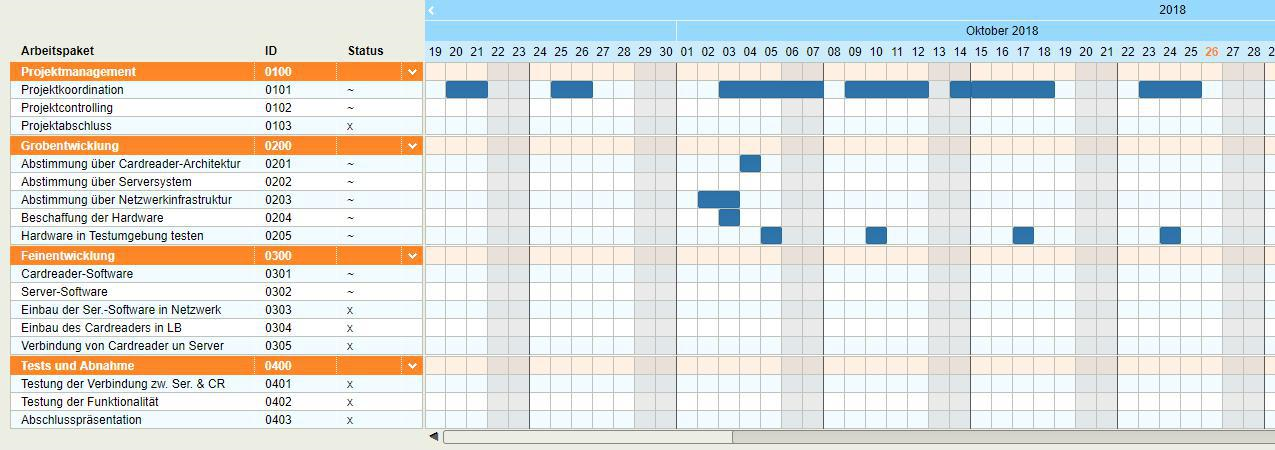
\includegraphics[angle=-90,scale=0.58]{images/balkenplan.png}
\end{center}
\vspace{1cm}
\newpage 

% Martin Wustinger
\subsection{Projektpersonaleinsatzplan}
\begingroup
\renewcommand*{\arraystretch}{1.1} % Abstand zwischen Zeilen
\begin{center}
\begin{scriptsize}
\begin{tabularx}{\textwidth}{|p{0.8cm}|p{2.2cm}|X|X|X|X|X|}
    \hline
    \multicolumn{7}{|c|}{\vspace{-0.02cm} \rowcolor{gray}} \\
    \multicolumn{7}{|c|}{\rowcolor{gray}\bfseries \normalsize \color{white} PROJEKTPERSONALEINSATZPLAN \vspace{-0.05cm}} \\
    \multicolumn{7}{|c|}{\rowcolor{gray}} \\
    \hline
    \textbf{PSP-} & \textbf{Phase/Arbeits-} &  \textbf{Ressourcen-} & \textbf{Planmenge} & \textbf{Adaptierte} & \textbf{Istmenge} & \textbf{Ausweichung}\\
    \textbf{Code} & \textbf{paket} &  \textbf{art} & \textbf{in \%} & \textbf{Planemenge} & \textbf{in \%} & \textbf{in \%}\\
    & & & & \textbf{in \%} & & \\
    \hline
    0101 & Projektkoordination & intern &7,5 & &6,9 & \\
    \hline
    0102 & Projektcontrolling & intern &5,4 & &0 & \\
    \hline
    0103 & Projektabschluss & intern &1,3 & &0 & \\
    \hline
    0201 & Abstimmung über Cardreader-Architektur & extern &2,1 & &0,8 & \\
    \hline
    0202 & Abstimmung über Serversystem-Architektur & extern &2,1 & &0 & \\
    \hline
    0203 & Abstimmung über Netzwerk-Infrastruktur & extern &2,5 & &0 & \\
    \hline
    0204 & Beschaffung der Hardware & extern &2,1 & &0,8 & \\
    \hline
    0205 & Hardware in Testumgebung testen & intern &4,1 & &7,9 & \\
    \hline
    0301 & Cardreader-Software & intern &10,4 & &0 & \\
    \hline
    0302 & Server-Software & intern &10,4 & &0 & \\
    \hline
    0303 & Einbau der Server-Software in Netzwerk & intern &6,3 & &0 & \\
    \hline
    0304 & Einbau der Cardreaders in LB & intern &2,1 & &0 & \\
    \hline
    0305 & Verbindung von Cardreader und Server & intern &5,8 & &0 & \\
    \hline
    0401 & Testung der Verbindung zw. Server und Cardreader & intern &6,3 & &0 & \\
    \hline
    0402 & Testung der Funktionalität & intern &6,3 & &0 & \\
    \hline
    0403 & Abschluss-Präsentation & intern &2,5 & &0 & \\
    \hline
\end{tabularx}
\end{scriptsize}
\end{center}
\endgroup

\newpage


\subsection{Projektkostenplan}



\begingroup
\renewcommand*{\arraystretch}{1.4} % Abstand zwischen Zeilen
\begin{center}
\begin{scriptsize}

\begin{longtable}{|p{1.6cm}|p{2.5cm}|c|c|c|p{2.3cm}|}
    \hline
    \multicolumn{6}{|c|}{\vspace{-0.05cm}\rowcolor{gray}} \\
    \multicolumn{6}{|c|}{\rowcolor{gray}\bfseries \normalsize \color{white} \:\:\:\:\:\:\:\:\:PROJEKTKOSTENPLAN\:\:\:\:\:\: \mybox[rounded corners]{mycol}{\:\:\:\:\:}\vspace{-0.0075cm}} \\
    \multicolumn{6}{|c|}{\rowcolor{gray}} \\
    \hline
    PSP-Code, & Kostenart & Plankosten & Adaptierte & Istkosten & Kostenabweichung\\
    AP- & & & Plankosten & & \\
    Bezeichnung & & & per....& &  \\
    \hline
    
    [0101] Projektkoordination& \tabitem Personal & 381.25€& & & \\
    \cline{2-6}
    & \tabitem Material & 5000€ & & & \\
    \cline{2-6}
    & \tabitem Fremdleistungen & & & & \\
    \cline{2-6}
    & \tabitem Sonstige & & & & \\
    \cline{2-6}
    & Gesamt & & & & \\
    \hline
    
    [0102]  Projektcontrolling & \tabitem Personal & 762.5€& & & \\
    \cline{2-6}
    & \tabitem Material & & & & \\
    \cline{2-6}
    & \tabitem Fremdleistungen & & & & \\
    \cline{2-6}
    & \tabitem Sonstige & & & & \\
    \cline{2-6}
    & Gesamt & & & & \\
    \hline
    
    [0103]  Projekt-Abschluss  & \tabitem Personal & 381.25€& & & \\
    \cline{2-6}
    & \tabitem Material & & & & \\
    \cline{2-6}
    & \tabitem Fremdleistungen & & & & \\
    \cline{2-6}
    & \tabitem Sonstige & & & & \\
    \cline{2-6}
    & Gesamt & & & & \\
    \hline
    
    
    [0201]  Abstimmung über Cardreader-Architektur & \tabitem Personal &381.25€ & & & \\
    \cline{2-6}
    & \tabitem Material & & & & \\
    \cline{2-6}
    & \tabitem Fremdleistungen & & & & \\
    \cline{2-6}
    & \tabitem Sonstige & & & & \\
    \cline{2-6}
    & Gesamt & & & & \\
    \hline
    
    [0202]  Abstimmung über Serversystem & \tabitem Personal & 381.25€& & & \\
    \cline{2-6}
    & \tabitem Material & & & & \\
    \cline{2-6}
    & \tabitem Fremdleistungen & & & & \\
    \cline{2-6}
    & \tabitem Sonstige & & & & \\
    \cline{2-6}
    & Gesamt & & & & \\
    \hline
    
    [0203]  Abstimmung über Netzwerkinfrastruktur & \tabitem Personal & 457.5€& & & \\
    \cline{2-6}
    & \tabitem Material & & & & \\
    \cline{2-6}
    & \tabitem Fremdleistungen & & & & \\
    \cline{2-6}
    & \tabitem Sonstige & & & & \\
    \cline{2-6}
    & Gesamt & & & & \\
    \hline
    
    [0204]  Beschaffung der Hardware & \tabitem Personal & 381.25€& & & \\
    \cline{2-6}
    & \tabitem Material & 75€ & & & \\
    \cline{2-6}
    & \tabitem Fremdleistungen & & & & \\
    \cline{2-6}
    & \tabitem Sonstige & & & & \\
    \cline{2-6}
    & Gesamt & & & & \\
    \hline
    
    [0205]  Hardware in Testumgebung testen & \tabitem Personal & 762.5€& & & \\
    \cline{2-6}
    & \tabitem Material & & & & \\
    \cline{2-6}
    & \tabitem Fremdleistungen & & & & \\
    \cline{2-6}
    & \tabitem Sonstige & & & & \\
    \cline{2-6}
    & Gesamt & & & & \\
    \hline
    
    [0301]  Cardreader-Software & \tabitem Personal &1906.25€ & & & \\
    \cline{2-6}
    & \tabitem Material & & & & \\
    \cline{2-6}
    & \tabitem Fremdleistungen & 1500€& & & \\
    \cline{2-6}
    & \tabitem Sonstige & & & & \\
    \cline{2-6}
    & Gesamt & & & & \\
    \hline
    
    [0302]  Server-Software & \tabitem Personal &1906.25€ & & & \\
    \cline{2-6}
    & \tabitem Material & & & & \\
    \cline{2-6}
    & \tabitem Fremdleistungen & & & & \\
    \cline{2-6}
    & \tabitem Sonstige & & & & \\
    \cline{2-6}
    & Gesamt & & & & \\
    \hline
    
    [0303]  Einbau der Server-Software in Netzwerk & \tabitem Personal &1143.75€ & & & \\
    \cline{2-6}
    & \tabitem Material & & & & \\
    \cline{2-6}
    & \tabitem Fremdleistungen & & & & \\
    \cline{2-6}
    & \tabitem Sonstige & & & & \\
    \cline{2-6}
    & Gesamt & & & & \\
    \hline
    
    [0304]  Einbau des Cardreaders in LB & \tabitem Personal &381.25€ & & & \\
    \cline{2-6}
    & \tabitem Material & & & & \\
    \cline{2-6}
    & \tabitem Fremdleistungen & & & & \\
    \cline{2-6}
    & \tabitem Sonstige & & & & \\
    \cline{2-6}
    & Gesamt & & & & \\
    \hline
    
    [0305]  Verbindung von Cardreader und Server & \tabitem Personal &1067.5€ & & & \\
    \cline{2-6}
    & \tabitem Material & & & & \\
    \cline{2-6}
    & \tabitem Fremdleistungen & & & & \\
    \cline{2-6}
    & \tabitem Sonstige & & & & \\
    \cline{2-6}
    & Gesamt & & & & \\
    \hline
    
    [0401]  Testung der Verbindung zwischen Cardreader \& Server & \tabitem Personal & 1601.25€& & & \\
    \cline{2-6}
    & \tabitem Material & & & & \\
    \cline{2-6}
    & \tabitem Fremdleistungen & & & & \\
    \cline{2-6}
    & \tabitem Sonstige & & & & \\
    \cline{2-6}
    & Gesamt & & & & \\
    \hline
    
    [0402]  Testung der Funktionalität & \tabitem Personal & 1601.25€& & & \\
    \cline{2-6}
    & \tabitem Material & & & & \\
    \cline{2-6}
    & \tabitem Fremdleistungen & & & & \\
    \cline{2-6}
    & \tabitem Sonstige & & & & \\
    \cline{2-6}
    & Gesamt & & & & \\
    \hline
    
    [0403]  Abschlusspräsentation & \tabitem Personal &762.5€ & & & \\
    \cline{2-6}
    & \tabitem Material & & & & \\
    \cline{2-6}
    & \tabitem Fremdleistungen & & & & \\
    \cline{2-6}
    & \tabitem Sonstige & & & & \\
    \cline{2-6}
    & Gesamt & & & & \\
    \hline
    Projektkosten & 20 833.75€& & & & \\
    \hline
    
    
\end{longtable}
\end{scriptsize}
\end{center}
\endgroup

\newpage


\subsection{Projektkommunikationsstrukturen}

\begingroup
\renewcommand*{\arraystretch}{1.1} % Abstand zwischen Zeilen
\begin{center}
\begin{scriptsize}
\begin{tabularx}{\textwidth}{|p{2.75cm}|p{4.3cm}|p{3cm}|l|X|}
    \hline
    \multicolumn{5}{|c|}{\rowcolor{gray}\vspace{-0.02cm}} \\
    \multicolumn{5}{|c|}{\rowcolor{gray}\bfseries \normalsize \color{white} Projektkommunikation\vspace{-0.05cm}} \\
    \multicolumn{5}{|c|}{\rowcolor{gray}} \\
    \hline
    \textbf{Bezeichnung} & \textbf{Ziele, Inhalte} & \textbf{Teilnehmer} & \textbf{Termine} & \textbf{Ort} \\
    & & & & \\
    \hline
    \multirow{2}{*}{\shortstack[l]{ProjektauftraggeberIn- \\ Sitzung}} & \multirow{6}{*}{
    \begin{minipage}{.3\textwidth} 
    \begin{flushleft}
        \begin{itemize} \vspace{0cm}  
         \item Diskussion Projektstatus, Abweichung im Projekt
         \item Entscheidungsfindung auf Basis der Projektcontrolling-Sitzung
         \item Freigabe Projektfortschrittsbericht
    \end{itemize}
    \end{flushleft}
    \end{minipage}} & \multirow{6}{*}{
    \begin{minipage}{.2\textwidth} \vspace{-1cm}
        ProjektauftraggeberIn, ProjektleiterIn, \\ Projektteam%(ev. SubteamleiterIn)
    \end{minipage}} & \multirow{6}{*}{
    \begin{minipage}{.1\textwidth} \vspace{-1.7cm}
        Bei Bedarf
    \end{minipage}} & \multirow{6}{*}{
    \begin{minipage}{.1\textwidth} \vspace{-1cm}
        TGM, H1131, H1132
    \end{minipage}}
    & & & & &\\
    & & & & \\
    & & & & \\
    & & & & \\
    & & & & \\
    & & & & \\
    \hline
    
    \multirow{2}{*}{\shortstack[l]{Projektcontrolling-
    \\Sitzung}} & \multirow{12}{*}{
    \begin{minipage}{.3\textwidth} 
    \begin{flushleft}
        \begin{itemize} \vspace{-0.cm}  
         \item Projektstatus
         \item Controlling Leistungsfortschritt, Termine und Ressourcen, Kosten
         \item Controlling der Umweltbeziehungen
         \item Soziales Projektcontrolling
         \item Diskussion übergeordneter Problemstellungen
         \item Entscheidungsaufbereitung für Projektauftraggeber-Sitzung
    \end{itemize} 
    \end{flushleft}
    \end{minipage}}  & \multirow{12}{*}{
    \begin{minipage}{.2\textwidth} \vspace{-2.99cm}
    	ProjektleiterIn, \\
        Projektteam, \\
        Projektcoach
    \end{minipage}} & \multirow{6}{*}{
    \begin{minipage}{.1\textwidth} \vspace{-1.2cm}
        Jeden Mittwoch
    \end{minipage}} & \multirow{6}{*}{
    \begin{minipage}{.1\textwidth} \vspace{-0.90cm}
        TGM,\\ H1132\\
    \end{minipage}}
    & & & & &\\
    & & & & \\
    & & & & \\
    & & & & \\
    & & & & \\
    & & & & \\
    & & & & \\
    & & & & \\
    & & & & \\& & & & \\
    & & & & \\& & & & \\
    \hline
    
    \shortstack[l]{Notfalls-Sitzung} & \multirow{4}{*}{
    \begin{minipage}{.3\textwidth} 
    \begin{flushleft}
        \begin{itemize} \vspace{0.2cm}  
         \item Projektcontrolling zum Gegenwirken von Risiken
         \item Diskussion inhaltlicher Problemstellungen
    \end{itemize}
    \end{flushleft}
    \end{minipage}} & \multirow{4}{*}{
    \begin{minipage}{.2\textwidth} \vspace{-0.1cm}
    	ProjektleiterIn, \\
        Projektteam, \\
        Projektcoach
    \end{minipage}} & \multirow{6}{*}{
    \begin{minipage}{.1\textwidth} \vspace{-1.55cm}
        Bei Bedarf
    \end{minipage}} & \multirow{6}{*}{
    \begin{minipage}{.1\textwidth} \vspace{-0.61cm}
        TGM,\\ H1132,\\
        Discord
    \end{minipage}}
    & & & & &\\
    & & & & \\
    & & & & \\
    & & & & \\
    \hline
\end{tabularx}
\end{scriptsize}
\end{center}
\endgroup

\newpage


\subsection{Projekt-\glqq Spielregeln \grqq}

\begingroup
\renewcommand*{\arraystretch}{1.1} % Abstand zwischen Zeilen
\begin{center}
\begin{scriptsize}
\begin{tabularx}{\textwidth}{|p{3cm}|p{3cm}|X|}
    \hline
    \rowcolor{gray} \normalsize \color{white} \textbf{Symbol} & \color{white} \normalsize \textbf{Spielregel} & \color{white} \normalsize \textbf{Beschreibung} \\
    \hline
    \multirow{4}{*}{\begin{minipage}{3cm}
    \begin{center}
        \vspace{0.5cm}
        
\includegraphics[width=40]{images/sr/1.png}
    \end{center}
    \end{minipage}} & Kommunikation 
    & Zur Kommunikation zwischen dem Projektteam und
    einzelnen Mitgliedern wird hauptsächlich Telegram
    verwendet, vereinzelt werden aber auch E-Mails
    verwendet. Kommunikationsmittel wie Telegram sollten
    primär für Absprachen und Fragen benutzt werden. Falls Dokumente, die nicht in Latex per Overleaf realisiert werden, verschickt werden müssen, soll das \gls{git}-Repository auf BitBucket dazu verwendet werden. Siehe Punkt Dateifreigabe. \\
    \hline 
    \multirow{4}{*}{\begin{minipage}{3cm}
    \begin{center}
        \vspace{0.15cm}
        
\includegraphics[width=50]{images/sr/2.png}
    \end{center}
    \end{minipage}} & Dateifreigabe
    & Projekt spezifische Dokumente, aber auch Projekt-Dateien
    wie Programmcodes und weiteres soll am \gls{git}-Repository auf BitBucket hochgeladen werden. Dokumentverkehr über
    Telegram sollte unterbunden werden. \\
    & & \\& & \\
    \hline
    \multirow{4}{*}{\begin{minipage}{3cm}
    \begin{center}
        \vspace{0.28cm}
        
\includegraphics[width=60]{images/sr/3.png}
    \end{center}
    \end{minipage}} & Zeitaufzeichnung &
    Nach jeder produktiven Arbeit für das Projekt soll die
    verstrichene Zeit dem Zeitaufzeichnungs-verantwortlichen
    Herrn Wustinger, gemeinsam mit der Beschreibung der
    durchgeführten Arbeit, übergeben werden.
    Alternativ kann man die Zeitaufzeichnung selber führen,
    dies muss aber gründlich und nachvollziehbar gemacht
    werden. \\
    \hline
    \begin{center}
        \vspace{0.5cm}
        \huge V\_.\_
    \end{center}& Versionierung &
    Jedem Dokument und jeder Datei muss eine Version
    zuordnungsbar sein. Bei Dokumenten muss ein
    Änderungsverzeichnis geführt werden, wo immer die
    Versionsnummer, Änderung und Autor ersichtlich sind.
    Dokumente und Dateien müssen mit der Versionsnummer
    im Format V„Hauptversion“. „Unterversion“ wie V1.0 oder
    V0.8 enden. Die Unterversion kann in Einzelfällen
    gestrichen werden, es wird aber dann in diesem Fällen
    geraten .0 zu verwenden. \newline Auf die Versionierung von Dokumeten wird im Kapitel Projekdokumentation mehr im Detail angegangen. \\
    \hline
    \multirow{4}{*}{\begin{minipage}{3cm}
    \begin{center}
        \vspace{0.0cm}
        
\includegraphics[width=50]{images/sr/4.png}
    \end{center}
    \end{minipage}} & Protokolle 
    & Für größere Besprechungen sollen immer Protokolle erstellt
    werden, die sich aus Datum, Teilnehmer, Sitzungsleiter,
    Ort, Hauptthema, Inhalt, Ergebnis gliedern. \\
    & & \\
    & & \\
    \hline
    \multirow{4}{*}{\begin{minipage}{3cm}
    \begin{center}
        \vspace{0.3cm}
        \centerline{\hspace{0.2cm}
\includegraphics[width=130]{images/sr/5.png}}
    \end{center}
    \end{minipage}} & Ein Team 
    & Die Projektteammitglieder sollen respektvoll miteinander
    umgehen und wirklich gemeinsam am Projekt arbeiten. 
    Jeder darf und soll Ideen für das Projekt vorschlagen.
    Diese sollen gemeinsam besprochen werden. \newline
    Jeder soll sich für seinen Projekt-Teil zuständig fühlen und
    an diesen sorgfältig und mit voller Dedikation arbeiten. \newline Jedes Mitglied soll voll hinter dem Projekt stehen. Um dies zu garantieren sollen Probleme sofort angesprochen
    werden und seriös ausdiskutiert werden. \\
    \hline
    
\end{tabularx}
\end{scriptsize}
\end{center}
\endgroup


\newpage 



\subsection{Projektrisikoanalyse}
\begingroup
\renewcommand*{\arraystretch}{1.1} % Abstand zwischen Zeilen
\begin{center}
\begin{tiny}
\begin{tabularx}{\textwidth}{|l|p{1.1cm}|X|l|l|l|p{0.5cm}|l|X|X|}
    \hline
    \multicolumn{10}{|c|}{\vspace{-0.02cm} \rowcolor{gray}} \\
    \multicolumn{10}{|c|}{\rowcolor{gray} \bfseries \normalsize \color{white} PROJEKTRISIKOANALYSE \vspace{-0.05cm}} \\
    \multicolumn{10}{|c|}{\rowcolor{gray}} \\
    \hline
    & & & & & & & & &\\
    & & Risiko- & & & Eintritts- & & & Präventive & Risiko-\\
    PSP- & Arbeitspaket- & beschreibung, & & Risiko- & wahrschein- & Risiko- & Ver- & korrektive & minimierungs- \\
    Code & bezeichnung & Ursache & Priorität & kosten & lichkeit & wert & zögerung & Maßnahmen & kosten \\
    \hline 
    (Code) & (Text) & (Text) & (Auswahl) & (Euro) & (Prozent) & (Euro) & (Wochen) & (Text) & (Euro) \\
    \hline
    [0303] & Einbau der Serv.-Software in Netzwerk & Schwierig- keiten beim Aufsetzen des Serversystems im Schulnetzwerk & 2 & €750 & 10\% & & 1 & Abstimmung mit IT-Service über vorhandene Netzwerkstruktur und Anweisungen um einen Server im Schulnetzwerk aufzusetzen &-\\
    \hline
    [0305]& Verbindung von Cardreader und Server & Netzwerkrout- ing-Probleme im Schulnetzwerk & 1 & €1200+ & 5\% & & 3+ & Absprache mit IT-Service über Netzwerk & -\\
    \hline
    [0305]& Verbindung von Cardreader und Server & Kommunika- tionsprobleme zwischen Cardreader und Server & 1 & €1200+ & 40\% & & 3+ & Absprache mit IT-Service über Netzwerk & -\\
    \hline
    [0301]& Cardreader-Software & Probleme beim Lesen von Kartendaten & 2 & €250 & 15\% & & <1 & Vergleich mit existierender Kartenleser Technologie, Absprache mit Kartenhersteller & €50\\
    \hline
    [0302]& Server-Software & Probleme bei der Zuordnung von Kartendaten zu Schulstunden & 2 & €750 & 30\% & & 2 & Absprache mit IT-Service und LDAP Betreiber & -\\
    \hline
    [0302]& Server-Software & Probleme bei der Übersetzung von Kartendaten zu Schüler-ID & 2 & €750 & 30\% & & 2 & Absprache mit IT-Service und LDAP Betreiber & -\\
    \hline
    & & Projektteilziele harmonisieren nicht miteinander & 3 & €350 & 5\% & & 1-2 & Vorausplanung mit Hilfe von Lehrern & -\\
    \hline
    & & Krankheitsbe- dingter Ausfall eines Teammitglieds & 2 & €900 & 80\% & & 2 & Gesundheits- zustand der Teammitglieder in Planungszeit einberechnen & -\\
    \hline
    & & Projektbudget wird nicht zur Verfügung gestellt & 1 & €150 & 95\% & & 0 & Quasi unausweichlich da Mittel der Schule durch Steuerskandal eingefroren wurden & €150\\
    \hline
    \multicolumn{2}{|l|}{Summe Projekt} & & & €6300 & & & 15+ & &€200\\
    \hline
\end{tabularx}
\end{tiny}
\end{center}
\endgroup
\begin{flushleft}
Die Priorität wird von eins an aufsteigend bewertet, wobei 1. die höchste Priorität besitzt.
\end{flushleft}
\newpage

% Martin Wustinger
\subsection{Projektdokumentation}

\begingroup
\renewcommand*{\arraystretch}{1.1} % Abstand zwischen Zeilen
\begin{center}
\begin{tabularx}{\textwidth}{|p{3.2cm}|X|}

    \hline
    \rowcolor{gray} \color{white}\textbf{Bereich} & \color{white}\textbf{Beschreibung} \\
    \hline
    Ablage & Alle Dokumente werden nach ihrer Vollendung auf der Elearning Plattform des TGMs hochgeladen. \\
    & \\
    \hline
    \multirow{2}{*}{\shortstack[l]{Zugriffs- \\ berechtigung}} & Alle Projekt-Teammitglieder haben dauerhaft Zugriff zu allen Dokumenten.\\
    & \\
    \hline
    Namenskonvention & Wie im Kapitel Spielregeln beschrieben, müssen alle Dokumente versioniert werden. Dies soll durch das Änderungsverzeichnis und den Dateinamen des jeweiligen Dokumentes ersichtlich sein. \newline \newline Dateinamen sollen wie folgt aufgebaut sein:  
    \newline 4AHIT\_LBVT\_Dokumentname\_V\_.\_ 
    \newline \newline wobei 4AHIT\_ nicht zwingend angegeben werden muss \\
    & \\
    \hline
    Spielregeln & Die Spielregeln des Projekts werden im Kapitel Spielregeln des Projekthandbuches genauer erläutert. An diese haben sich alle Projekt-Team-Mitglieder zu halten.\\
    & \\
    \hline
\end{tabularx}
\end{center}
\endgroup

\newpage

\section{Projektstart}
\subsection{Protokolle - Projektstart}
%\subsubsection{Projektstart-Workshop}
%\subsubsection{Follow-up-Workshop}
%\subsubsection{Projektauftraggeber-Sitzung}
\projektprotokoll{001
}{
26.09.2018
}{
\begin{itemize} \vspace{0.1cm}
         \item Christoph Roschger
        \item Manuel Kisser
        \item Kacper Urbaniec
        \item Moritz Welsch
        \item Martin Wustinger
         \vspace{0.2cm}
     \end{itemize}
}{
Christoph Roschger
}{
TGM
}{
Durchbesprechung des Projektantrages und Abgrenzung der Projektinhalte
}{
Der Projektantrag wurde durchgegangen und es wurde die Ausgangssituation und vorhandene Infrastruktur des Projekets weiter erläutert
}{
\begin{itemize} \vspace{0.1cm}
            \item Mit Voranmeldungssoftware kann das Projekt eventuell um ein Semester verlängert werden
            \item Im Projektantrag den Text Für den Unterricht \glqq Authentifizieren\grqq\:auf \glqq Anmelden\grqq\:ändern
            \item Vorhandener Kartenleser funktioniert, allerdings sehr langsam (evt. wegen Volt-einstellungen)
            \item Von den Werkstätten kann eventuell das Gehäuse für die Kartenleser bezogen werden
            \item Zum Testen des Kartenleser soll der Name von dem Educard-Inhaber ausgesprochen werden (vorhandenes Skript), in der Praxis kann auch eine Lämpchen eingesetzt werden.
            \item Es gibt derzeit keine Webserverkosten, da es schon einen Webserver gibt.
            \item Definition von Kartenleser = Raspberry (oder gleichwertiger Kleincomputer) + Kartenleser(NFC) + SD-Card + Stromkabel
            \item Eigener Zugang für Wlan/\gls{lba}
            \item Zum Testen einen extra Server aufsetzen, Prof. Roschger würde den mit seiner vorhandenen Software aufsetzen
            \item Educard liefert nur ID, (0002) -\char62{} muss in einen Benutzer umgewandelt werden
            \item Kosten auf 75 € hochsetzen, Beispiel: Raspberry(50)+Kartenleser(20)
            \vspace{0.2cm}
        \end{itemize}
}
\newpage
\newpage


\section{Projektkoordination}

\subsection{Abnahme Arbeitspakete}

\begingroup
\begin{small}
\renewcommand*{\arraystretch}{1.1} % Abstand zwischen Zeilen
\begin{center}
\begin{tabularx}{\textwidth}{|l|p{3.5cm}|X|l|l|l|}
    \hline
    \multicolumn{6}{|c|}{\vspace{-0.05} \rowcolor{gray}} \\
    \multicolumn{6}{|c|}{\rowcolor{gray} \bfseries \normalsize \color{white} ABNAHME ARBEITSPAKETE \vspace{-0.5}} \\
    \multicolumn{6}{|c|}{\rowcolor{gray}} \\
    \hline
    \normalsize \textbf{PSP-} & \normalsize \textbf{Arbeitspaket} & \normalsize \textbf{AP-Verantw.} & \normalsize \textbf{Datum} & \normalsize \textbf{Abnahme} & \normalsize \textbf{Unterschrift} \\
    \normalsize \textbf{Code} & & &  & \normalsize \textbf{durch}& \\
    \hline
    101& Projektkoordination &Kacper Urbaniec&&&\\
    \hline
    102& Projektcontrolling &Kacper Urbaniec&&&\\
    \hline
    103& Projektabschluss &Kacper Urbaniec&&&\\
    \hline
    201& Abstimmung über Cardreader-Architektur &Manuel Kisser&&&\\
    \hline
    202& Abstimmung über Serversystem-Architektur &Manuel Kisser&&&\\
    \hline
    203& Abstimmung über Netzwerk-Infrastruktur &Manuel Kisser&&&\\
    \hline
    204& Beschaffung der Hardware &Manuel Kisser&&&\\
    \hline
    205& Hardware in Testumgebung testen &Manuel Kisser&&&\\
    \hline
    301& Cardreader-Software &Moritz Welsch&&&\\
    \hline
    302& Server-Software &Martin Wustinger&&&\\
    \hline
    303& Einbau der Server-Software in Netzwerk &Moritz Welsch&&&\\
    \hline
    304& Einbau der Cardreaders in LB &Kacper Urbaniec&&&\\
    \hline
    305& Verbindung von Cardreader und Server &Moritz Welsch&&&\\
    \hline
    401& Testung der Verbindung zw. Server und Cardreader &Moritz Welsch&&&\\
    \hline
    402& Testung der Funktionalität &Martin Wustinger&&&\\
    \hline
    403& Abschluss-Präsentation &Kacper Urbaniec&&&\\
    \hline

\end{tabularx}
\end{center}
\end{small}
\endgroup

\newpage

\subsection{Protokolle - Projektkoordination}




\projektprotokoll{002
}{
26.09.2018
}{
\item IT-Service-Personal (Name unbekannt)
        \item Manuel Kisser
        \item Kacper Urbaniec
        \item Moritz Welsch
        \item Martin Wustinger
}{
IT-Service
}{
TGM
}{
Das LBVT wurde dem IT-Service vorgestellt
}{
LBVT wurde mit dem IT-Service durchgegangen und es wurden mögliche Umsetzungsmöglichkeiten besprochen
}{
\begin{itemize} \vspace{0.1cm}
            \item Herr Manuel Kisser wurde zum Kommunikationsleiter zwischen Projektteam und IT-Service bestimmt. 
            \item In der nächsten Zeit wird vom IT-Service ein Netzwerk-Account erstellt, um damit einen Kartenlesers im Schulnetzwerk anzumelden.
            \item Die Serversitation ist weiterhin unklar, denn das IT-Service betreut nicht den Elearning-Server. Deshalb soll sich das Projektteam an Professor List wenden.
            \item Für eine Testumgebung könnte der Projekteserver eingesetzt werden, ebenfalls von Professor List betreut.
            \item IT-Service kann Educards nicht zuordnen, daher muss einen andere Möglichkeit für das Auslesen von Daten gefunden werden.
            \vspace{0.2cm}
        \end{itemize}
}
\newpage
\begin{center}
\begin{footnotesize}
\begingroup
\renewcommand*{\arraystretch}{1.45} % Abstand zwischen Zeilen
\begin{tabularx}{\textwidth}{|p{2cm}|X|}
    \hline
    \multicolumn{2}{|c|}{\vspace{-0.1cm}\rowcolor{gray}} \\
    \multicolumn{2}{|c|}{\rowcolor{gray}\bfseries \normalsize \color{white} Projekt-Sitzungs-Protokoll 003 \vspace{-0.01cm}} \\
    \multicolumn{2}{|c|}{\rowcolor{gray}} \\
    \hline
    \textbf{Datum} & 03.10.2018 überarbeitet am 05.10.2018 \\
    \hline
    \textbf{Teilnehmer} & 
    \begin{minipage}{.6\textwidth} 
     \begin{flushleft}
        \begin{itemize} \vspace{0.1cm}
        \item Manuel Kisser
        \item Kacper Urbaniec
        \item Moritz Welsch
        \item Martin Wustinger
         \vspace{0.2cm}
     \end{itemize}
     \end{flushleft}
     \end{minipage} \\
     \hline
     \textbf{Sitzungsleiter} & Kacper Urbaniec \\
     \hline
     \textbf{Ort} & TGM \\
     \hline
     \textbf{Hauptthema} & Produktfunktionsablauf  \\
     \hline
     \textbf{Inhalt} & Der Produktfunktionsablauf wurde im Detail durchgegegangen um Funktionen, Daten, Leistungen, etc. definieren zu können \\
     \hline
     \textbf{Ergebnis} & 
     \begin{minipage}{.81\textwidth} 
     \begin{flushleft}
        \vspace{0.1cm}
        \textbf{Produktfunktionen} \\
        Server Funktionen \\
        \begin{itemize}
            \item Datenbank um Anmeldedaten zu speichern
            \item Anmeldedaten empfangen 
            \item Anmeldedaten in den Server eintragen (ID in Name umwandeln und Klasse heraussuchen, überprüfen ob Eintrag schon vorhanden)
            \item Anwesenheit muss an die Lernbüroapplikation gesendet/eingetragen werden
            \item Klassenliste einlesen
            \item Successfull Acknowledge Paket (Verschlüsselt) an Kartenleser senden
            \item Entschlüsselung der Request
        \end{itemize}
        Kartenleser Funktionen \\
        \begin{itemize}
            \item Karte einlesen
            \item Daten im Zwischenspeicher speichern
            \item Inhalt des Zwischenspeichers senden (gleich senden, alle 10 Minuten falls ungesendet)
            \item Zwischenspeicher löschen (Sobald eine Successfull Acknowledge empfangen wurde, Zwischenspeicher löschen)
            \item Feedback nach Anmeldung
            \item Doppelte Einträge aus Kartenleser-Datenbank löschen
            \item Verschlüsselung der Request
            \item Entschlüsselung der Acknowledge Paket
        \end{itemize}
        Grafische Oberfläche in der \gls{lba} \\
        \begin{itemize}
            \item Anzeigen der Kartenleserdaten (ID, Raumzuteilung, etc.)
            \item Kartenleser Raum zuordnen
        \end{itemize}
    \textbf{Produktdaten} \\
    Mögliche Struktur für Serverdaten:
    \begin{itemize}
    \item Klassenlisten
    \item Dictionary: Id zu Name
    \item Anwesenheitsdatenliste
    
    \begin{itemize}
    \item PK Datum
    \item PK ID
    \item Klasse
    \item Name
    \item Anwesend j/n
    \end{itemize} \end{itemize} \\
    \end{flushleft}
     \end{minipage} \\
    
\end{tabularx}
\endgroup
\end{footnotesize}
\end{center}

\begin{center}
\begin{footnotesize}
\begingroup
\renewcommand*{\arraystretch}{1.45} % Abstand zwischen Zeilen
\begin{tabularx}{\textwidth}{|p{2cm}|X|} 
     & 
     \begin{minipage}{.81\textwidth} 
     \begin{flushleft}
 
    Mögliche Struktur für Kartenleserdaten (REQUEST-Messages):
    \begin{itemize}
        \item Datenliste 
        \begin{itemize}
            \item Datum 
            \item ID
        \end{itemize}
    \end{itemize}
    
    Interne Kartenleserdaten (für Server und GUI):
    
    \begin{itemize}
        \item Kartenleser-ID
        \item Raumzuteilung
    \end{itemize}
    
    \textbf{NICE TO HAVES} \\
    \begin{itemize}
        \item Alle Klassen der Abteilung IT sind mit Kartenlesern ausgestattet
        \item Die Lernbüroapplikation hat eine Voranmeldungssoftware, in der sich Lernbüroschüler per Website zeitlich vor den Unterrichtseinheiten für einen Gegenstand eintragen können
        \item Eine Abmelde-Funktion implementieren
    \end{itemize}
    \vspace{0.2cm}
     \end{flushleft}
     \end{minipage} \\
     \hline
    
\end{tabularx}
\endgroup
\end{footnotesize}
\end{center}
\newpage
\projektprotokoll{004
}{
03.10.2018
}{
\item Christoph Roschger
        \item Manuel Kisser
        \item Kacper Urbaniec
        \item Moritz Welsch
        \item Martin Wustinger
}{
Christoph Roschger
}{
TGM
}{
Produktfunktionen mit Autraggeber besprochen
}{
Besprechung der Produktfunktionen und  Beschaffung vom Kartenleser
}{
\begin{itemize} \vspace{0.1cm}
            \item Vormittag und Nachmittag im Lernbüro sind Zeitblöcke
            \item Anmeldung für diesen Block
            \item Raum in dem der Raspberry steht muss festlegbar sein
            \item Anhand von Raum mit Stundenplan verbinden um Dauer herauszufinden
            \item Direkte integration mit der Software der \gls{lba}
            \item Hardware wurde dem Projektteam bereitgestellt (Raspberry Pi mit NFC-Reader)
            \item Unter \texttt{/root} am Raspberry Pi sind alle derzeit vorhandenen Skripte zu finden
            \item Skript \texttt{heartbeat} für Senden zuständig
            \item Kartenleser soll immer Daten senden wenn sich ein Schüler anmeldet, damit die Lehrer dies gleich sehen in der \gls{lba} sehen können
            \item Modellname: \texttt{PN532}
            \item Zugangsdaten: \texttt{root}:\texttt{1234}
            \item Neue Funktion: \glqq Karte anwählen\grqq\: -\char62{} Schüler kommt mit Karte zum \gls{lbvt} und die Karte wird nachher eindeutig dem Schüler zugewiesen
            \item Zum Projekt soll ein Kartenleser-Gehäuse als Leistung hinzugefügt werden
            \vspace{0.2cm}
        \end{itemize}
}
\newpage
\projektprotokoll{005
}{
04.10.2018
}{
 \item Dominik Fürnsin
            \item Kacper Urbaniec
            \item Moritz Welsch
            \item Martin Wustinger
}{
 Dominik Fürnsin
}{
TGM
}{
Umsetzung des \gls{lbvt}
}{
Mit Fachlehrer Fürnsin gemeinsam Möglichkeiten zur Umsetzung des \gls{lbvt} im Schulnetzwerk gesucht
}{
\begin{itemize} \vspace{0.1cm}
            \item Solange das Projekt sich in der Umsetzungsphase befindet, sollen die Kartenleser die Accounts des Projektteam, zum Anmelden im Schulnetzwerk, verwenden
            \item In Endphase kann dann entsprechende Umgebung mit eigenen Accounts für Kartenleser realisiert werden
            \item Service-User mit eigenem VLAN, nur Zugang auf Server
            \item Falls es Probleme mit WPA2-PEAP, dann kann man das Gäste WLAN benutzen
            \item Gehäuse evt. mit 3-D Drucker?
            \item Evt. ein Akku-Pack für die Portabilität des Kartenlesers nutzen
            \item Evt. den Kartenleser mit einem Schalter erweitern, damit sich Schüler durch Knopfdruck früher abmelden können
            \item Kartenleser mit Touchscreen für Raumeingabe, wenn mit Akkupack genutz wird, ansonsten Risiko, dass Kartenleser vertauscht werden
            \item Idee, dass die Raum-Zuteilung des Kartenleser mittels NFC-Tags programmierbar ist
            \item Web-Interface damit der Raspberry einem Raum zugeordnet wird
            \vspace{0.2cm}
        \end{itemize}
}
\newpage
\projektprotokoll{ 006
}{
05.10.2018
}{
\item Kacper Urbaniec
            \item Moritz Welsch
            \item Martin Wustinger
}{
 Kacper Urbaniec
}{
TGM
}{
Projektantrag und Technologie zum Umwandeln der Schülerkarten-ID
}{
Notwendigkeit den Projektantrag zu überarbeiten wurde besprochen und Ideen zur Umwandlung der ID wurden gesucht
}{
\begin{itemize} \vspace{0.1cm}
            \item Projektteilziele, Wirkung, Nutzen, Projekteinnahmen und Wirtschaftlichkeit überarbeitet \item Einteilung, wer welchen Teil in den Dokumenten aktualisieren soll, wurde unternommen
            \item Dominik Fürnsin muss in Zukunf befragt werden, ob Projektteam Zugang zum Druckernetzwerk bekommt, um die Schülerkarten in Benutzernamen umzuwandeln zu können
            
            \vspace{0.2cm}
        \end{itemize}
}
\newpage
\projektprotokoll{ 007
}{
24.10.2018
}{
\item Moritz Welsch
            \item Martin Wustinger
            \item Manuel Kisser
}{
Manuel Kisser
}{
TGM
}{
Variantenbildung
}{
Variantenbildung für die Machbarkeitsstudie wurde unternommen
}{
\begin{itemize} \vspace{0.1cm}
            \item ZMQ wird verwendet
            \item Input-Script -\char62{} DB \char60{}- Output Script-\char62{} LDAP
            \item Sicherheit bei ZMQ?
            \item Zertifikatbasierte Sicherheit (automatisiert)
            \item Ubuntu-Server wird verwendet
            \item Docker wird in Überlegung gezogen
            \item Nicht IP-basiertes System (DDNS oder über LDAP einen Server-Namen)
            \item LDAP um Schüler den Klassen zuzuordnen
            \item DB evt. außerhalb des Docker-images bzw. eigenes Docker-img
            \item Web-Interface als letztes
            \item Web-Interface zur Raumeinteilung wird am ZPS bereitgestellt
            
            \vspace{0.2cm}
        \end{itemize}
}
\newpage
\projektprotokoll{ 008
}{
    07.11.2018
}{
\item Moritz Welsch
            \item Martin Wustinger
            \item Kacper Urbaniec
}{
 Moritz Welsch
}{
TGM
}{
Funktionen und Technologien des \gls{zps}
}{
Die Funktionen und dazu verwendeten Technologien des \gls{zps} werden besprochen
}{
\begin{itemize} \vspace{0.1cm}
            \item \gls{zps} hat Python-Input Script welches die gesendeten Daten mit ZMQ einließt und in die DB einschreibt
            \item Als Datenbank am \gls{zps} wird MariaDB verwendet
            \item Auf dem \gls{zps} wird für die Website PHP  verwendet, da der Zugriff auf eine Datenbank simpel ist.
            \item NGINX wird am \gls{zps} als Webserver verwendet.
            \item Python wird verwendet um Daten vom ZPS an das LBA zu senden
            \vspace{0.2cm}
        \end{itemize}
}
\newpage
\projektprotokoll{009
}{14.11.2018
}{
\item Moritz Welsch
            \item Martin Wustinger
            \item Kacper Urbaniec
            \item Manuel Kisser
            \item Stefan Zakall
}{
    Manuel Kisser
}{
    TGM
}{
 Projektmotivation und Sicherheit
}{
Die Funktionen und dazu verwendeten Technologien des \gls{zps} werden besprochen
}{
\begin{itemize} \vspace{0.1cm}
            \item Die Datenbank des Kartenlesers muss abgeändert werden
            \item Auf dem \gls{lba} wird, wenn möglich, das Unterrichtsfach dynamisch eingetragen
            \item Ein Zertifikat wird auf dem Kartenleser gespeichert, um dessen Echtheit zu überprüfen
            \item Kacper Urbaniec hat bereits seine geschätze Stundenanzahl erreicht
            \vspace{0.2cm}
        \end{itemize}
}


\newpage
\projektprotokoll{
    010
}{
    23.11.2011
}{
    \item Moritz Welsch
    \item Martin Wustinger
    \item Kacper Urbaniec
    \item Manuel Kisser
}{
    Manuel Kisser
}{
    TGM
}{
    Anstehende Arbeit, Meilensteine 28.11.2018
}{
    Arbeitsaufteilung der anstehenden Arbeit für den Meilenstein am 28.11.2018
}{
     \begin{itemize} \vspace{0.1cm}
            \item Abstimmung über Datenpakete
            \item Aufgabenverteilung:
            \begin{itemize} [leftmargin=15mm] 
                \item [Kisser] Kartenleser
                \item [Urbaniec] Website, Login
                \item [Welsch] Zertifikate-Autorität
                \item [Wustinger] ZPS-Datenverarbeitung
            \end{itemize}
            \vspace{0.2cm}
        \end{itemize}
}
\newpage
\newpage
\projektprotokoll{
    011
}{
    05.12.2011
}{
    \item Moritz Welsch
    \item Martin Wustinger
    \item Kacper Urbaniec
    \item Manuel Kisser
    \item Christoph Roschger
}{
    Martin Wustinger
}{
    TGM
}{
    Konzeptbesprechung
}{
    Überlegen des Konzepts da der Django-Server bereitgestellt wurde
}{
     \begin{itemize} \vspace{0.1cm}
            \item ZPS bleibt bestehen
            \item Am Django-Server wird so wenig wie möglich verändert
            \item Verbindung zwischen ZPS und Django muss realisiert werden
            \item Re-validierung der Kartenlesersoftwarearchitektur
            \vspace{0.2cm}
        \end{itemize}
}

\newpage
\projektprotokoll{
    012
}{
    12.12.2011
}{
    \item Moritz Welsch
    \item Martin Wustinger
    \item Kacper Urbaniec
    \item Manuel Kisser
    \item Michael Fischer
    \item Christoph Roschger
}{
    Michael Fischer
}{
    TGM
}{
    Mapping EDU-Cards
}{
    Besprechung mit IT-Service von EDU-Cards mapping zu Schüler-ID
}{
     \begin{itemize} \vspace{0.1cm}
            \item Klären mit Abteilungsvorstand ob Projektteam Karten-Mapping realisiert
            \item Oder: Roschger klärt das weitere Verfahren mit dem Mapping und informiert uns
            \item Idee für Roschger bzgl \gls{lba}: In der DB werden nur Karten-IDs gespeichert, welche dann erst beim Aufruf vom Front-End-Oberfläche mit dem Schüler gemappt werden. Eventuelles Problem wenn der Schüler eine neue Karte bekommt.
            \vspace{0.2cm}
        \end{itemize}
}

\newpage
\section{Projektcontrolling}

\subsection{Aktueller Projektfortschrittsbericht}

\begingroup
\renewcommand*{\arraystretch}{1.1} % Abstand zwischen Zeilen
\begin{center}
\begin{scriptsize}
\begin{tabularx}{\textwidth}{|p{8cm}|X|}
    \hline
    \multicolumn{2}{|c|}{\vspace{-0.02cm} \rowcolor{gray}} \\
    \multicolumn{2}{|c|}{\rowcolor{gray} \bfseries \normalsize \color{white} PROJEKTFORTSCHRITTSBERICHT \vspace{-0.05cm}} \\
    \multicolumn{2}{|c|}{\rowcolor{gray} \bfseries \normalsize \color{white} per 26.10.2018 \vspace{-0.05cm}} \\
    \multicolumn{2}{|c|}{\rowcolor{gray}} \\
    \hline
    \multicolumn{1}{|p{6cm}|}{\begin{minipage}{1cm} 
\includegraphics[width=40]{images/thing.PNG}\end{minipage} \hfill \begin{minipage}{4cm}\vspace{0.5cm}Projektkrise\vspace{0.3cm} \\ \vspace{0.3cm}Projekt in Schwierigkeiten \\ Projekt planmäßig 
\color{Green}\surd \vspace{0.4cm} \end{minipage}} & \begin{minipage}{5.3cm}\textbf{\hspace{-1mm}1) Gesamtstatus} \\ 
    \begin{flushleft}
        \begin{itemize} \vspace{-0.5cm}  
         \item \:[0101], [0201] - [0203], [0301], [0302] in Arbeit
    \end{itemize}
    \end{flushleft}
    \end{minipage}\\
    \hline
    \textbf{2) Status Ziele} & \textbf{Maßnahmen:}\\
    \begin{minipage}{.58\textwidth} 
    \begin{flushleft}
        \begin{itemize} \vspace{0cm}  
        \item \:[0101] Es wurden teilweise Dokumete erstellt bzw sind in Arbeit
         \item \:[0201] Es wurde begonnen an der Abstimmung der Cardreader Arichtektur zu arbeiten
         \item \:[0202] Es wurde begonnen an der Abstimmung der Serversysteme zu arbeiten
         \item \:[0203] Es wurde begonnen an der Abstimmung der Netzwerkinfrastruktur zu arbeiten
         \vspace{0.2cm}
    \end{itemize}
    \end{flushleft}
    \end{minipage} &
    \begin{minipage}{.58\textwidth} 
    \begin{flushleft}
        \begin{itemize} \vspace{-2.3cm}  
         \item \text{Keine}
    \end{itemize}
    \end{flushleft}
    \end{minipage} \\
    \hline
    \textbf{3) Status Leistungsfortschritt} & \textbf{Maßnahmen:}\\
    \begin{minipage}{.56\textwidth} 
    \begin{flushleft}
        \begin{itemize} \vspace{0cm}  
        \item \:[0101] 
        Das Projekthandbuch und die Machbarkeitsstudie sind zum Großteil fertig, das Pflichtenheft wurde begonnen
         \item \:[0201]/[0203]
            Die Abstimmung der Kartenleser-Architektur, des Serversystemes und der Netzwerkinfrastruktur sind in Arbeit
         \item \:[0202]
           Es wird momentan evaluiert und getestet welche Server-Software verwendet werden soll
            \item \:[0204] Teile der Hardware wurden schon beschaffen, derzeit wird evaluiert ob die vorhandenen Server, als Grundlage für das \gls{zps} verwendet werden können
         \item \:[0205], [0301] Kartenleser wurde in einer Testumgebung zum Laufen gebracht und es wurde begonnen Software für diesen zu erstellen
            \vspace{0.2cm}
    \end{itemize}
    \end{flushleft}
    \end{minipage} &
    \begin{minipage}{.4\textwidth} 
    \begin{flushleft}
        \begin{itemize} \vspace{-4cm}  
          \item \text{Keine}
    \end{itemize}
    \end{flushleft}
    \end{minipage} \\
    \hline
    \textbf{4) Status Termine} & \textbf{Maßnahmen:}\\
    \begin{minipage}{.58\textwidth} 
    \begin{flushleft}
        \begin{itemize} \vspace{-1.0cm}  
        \item \textbf{Alle benötigten Dokumente und Hefte sind fertig:} \newline Der Meilenstein mit 21.09.2018 wurde nicht eingehalten
         \item Die darauf folgenden Meilensteine können demnach ebenfalls nicht eingehalten werden
         \vspace{0.2cm}
         
    \end{itemize}
    \end{flushleft}
    \end{minipage} &
    \begin{minipage}{.4\textwidth} 
    \begin{flushleft}
        \begin{itemize} \vspace{0cm}  
         \item Da der Meilenstein nicht eingehalten werden konnte, müssen die nachfolgenden Termine nach hinten verschoben werden
         \item Es ist realistisch, dass einzelne Meilensteine parallel geführt werden können, deshalb bleibt der Termin für das Projekt-Ende unverändert \vspace{0.2cm}
    \end{itemize}
    \end{flushleft}
    \end{minipage} \\
    \hline
    \textbf{5) Status Ressourcen/Kosten} & \textbf{Maßnahmen:}\\
    \begin{minipage}{.58\textwidth} 
    \begin{flushleft}
        \begin{itemize} \vspace{0cm}  
         %\item Die Ressourcen und Kosten verlaufen besser als prognostiziert
         \item Kosten für Kartenleser von Projektauftraggeber schon gedeckt
         \item \gls{zps} wird höchstwahrscheinlich einem bestehenden Server hinzugefügt, was die Server-Kosten deutlich verringert \vspace{0.2cm}
    \end{itemize}
    \end{flushleft}
    \end{minipage} &
    \begin{minipage}{.4\textwidth} 
    \begin{flushleft}
        \begin{itemize} \vspace{-0.9cm}  
         \item Keine
    \end{itemize}
    \end{flushleft}
    \end{minipage} \\
    \hline
    \textbf{6) Status Kontext} & \textbf{Maßnahmen:}\\
    \begin{minipage}{.555\textwidth} 
    \begin{flushleft}
        \begin{itemize} \vspace{0cm}  
        \item Auftraggeber steht voll hinter dem Projekte und hilft bei Problemen und Organisation
        \item Aus Erfahrungen aus dem letzten Projekt, muss am Projekthandbuch sauberer gearbeitet werden \vspace{0.2cm}
         %\item \:[0201-0203] Die Abstimmung der Kartenleser-Architektur, des Serversystemes und der Netzwerkinfrastruktur sind in Arbeit
         %\item \:[0204] Teile der Hardware wurden schon beschaffen, derzeit wird evaluiert ob die vorhandenen Server, als Grundlage für das \gls{zps} verwendet werden können
         %\item \:[0205], [0301] Kartenleser wurde in einer Testumgebung zum Laufen gebracht und es wurde begonnen Software für diesen zu erstellen \vspace{0.2cm}
    \end{itemize}
    \end{flushleft}
    \end{minipage} &
    \begin{minipage}{.4\textwidth} 
    \begin{flushleft}
        \begin{itemize} \vspace{-0.5cm}  
         \item Um die korrekte Ausführung des Projekthandbuch zu gewährleisten, wird es jetzt öfter aktualisiert und angepasst 
    \end{itemize}
    \end{flushleft}
    \end{minipage} \\
    \hline
    \textbf{7) Status Organisation/Kultur} & \textbf{Maßnahmen:}\\
    \begin{minipage}{.57\textwidth} 
    \begin{flushleft}
        \begin{itemize} \vspace{0cm}  
         \item Arbeit und Kommunikation im Projektteam verläuft sehr \\ positiv ab, Arbeitsmoral ist gegeben
         \vspace{0.2cm}
    \end{itemize}
    \end{flushleft}
    \end{minipage} &
    \begin{minipage}{.4\textwidth} 
    \begin{flushleft}
        \begin{itemize} \vspace{-0.3cm}  
         \item Keine
         \vspace{0.2cm}
    \end{itemize}
    \end{flushleft}
    \end{minipage} \\
    \hline
\end{tabularx}
\end{scriptsize}
\end{center}
\endgroup

\newpage

\begingroup
\renewcommand*{\arraystretch}{1.1} % Abstand zwischen Zeilen
\begin{center}
\begin{scriptsize}
\begin{tabularx}{\textwidth}{|p{8cm}|X|}
    \hline
    \multicolumn{2}{|c|}{\vspace{-0.02cm} \rowcolor{gray}} \\
    \multicolumn{2}{|c|}{\rowcolor{gray} \bfseries \normalsize \color{white} PROJEKTFORTSCHRITTSBERICHT \vspace{-0.05cm}} \\
    \multicolumn{2}{|c|}{\rowcolor{gray} \bfseries \normalsize \color{white} per 14.11.2018 \vspace{-0.05cm}} \\
    \multicolumn{2}{|c|}{\rowcolor{gray}} \\
    \hline
    \multicolumn{1}{|p{6cm}|}{\begin{minipage}{1cm} 
\includegraphics[width=40]{images/thing.PNG}\end{minipage} \hfill \begin{minipage}{4cm}\vspace{0.5cm}Projektkrise\vspace{0.3cm} \\ \vspace{0.3cm}Projekt in Schwierigkeiten \\ Projekt planmäßig 
\color{Green}\surd \vspace{0.4cm} \end{minipage}} & \begin{minipage}{5.3cm}\textbf{\hspace{-1mm}1) Gesamtstatus} \\ 
    \begin{flushleft}
        \begin{itemize} \vspace{-0.5cm}  
        \item \:[201] - [203] fertig
         \item \:[0301], [0302] in Arbeit
    \end{itemize}
    \end{flushleft}
    \end{minipage}\\
    \hline
    \textbf{2) Status Ziele} & \textbf{Maßnahmen:}\\
    \begin{minipage}{.58\textwidth} 
    \begin{flushleft}
        \begin{itemize} \vspace{0cm}  
         \item \:[0301] Die Kartenleser-Software ist aktiv in Entwicklung
         \item \:[0302] Serverseitige-Software ist aktiv in Entwicklung, außer-\\ dem wurde Zugang zum \gls{lba} ersucht
         %\item \:[0201] Es wurde begonnen an der Abstimmung der Netzwerkinfrastruktur zu arbeiten
         \vspace{0.2cm}
    \end{itemize}
    \end{flushleft}
    \end{minipage} &
    \begin{minipage}{.58\textwidth} 
    \begin{flushleft}
        \begin{itemize} \vspace{-1cm}  
         \item \text{Keine}
    \end{itemize}
    \end{flushleft}
    \end{minipage} \\
    \hline
    \textbf{3) Status Leistungsfortschritt} & \textbf{Maßnahmen:}\\
    \begin{minipage}{.56\textwidth} 
    \begin{flushleft}
        \begin{itemize} \vspace{0cm}  
         \item \:[0301] \\
             Datenbank befindet sich in Implementationsphase
             Sicherheitskonzepte werden schrittweise implementiert
                 
         \item \:[0302] \\
             Das Input-Script, zum Einlesen der Daten über ZmQ-Schnittstelle ist fast fertig \\
             Stundenpläne können per Python-Script abgerufen und zur Weiterverarbeitung serialisiert werden
            \vspace{0.2cm}
    \end{itemize}
    \end{flushleft}
    \end{minipage} &
    \begin{minipage}{.4\textwidth} 
    \begin{flushleft}
        \begin{itemize} \vspace{-2.65cm}  
          \item \text{Keine}
    \end{itemize}
    \end{flushleft}
    \end{minipage} \\
    \hline
    \textbf{4) Status Termine} & \textbf{Maßnahmen:}\\
    \begin{minipage}{.57\textwidth} 
    \begin{flushleft}
        \begin{itemize}  
        \item Alle benötigten Dokumente und Hefte sind fertig
        \item Diverse Abstimmungen sind abgeschlossen
        \item Bestimmung der \gls{lbvt}-Hardware Spezifikationen und deren Bestellung kann nicht abgeschlossen werden, da die \gls{zps}-Hardware vom Auftraggeber noch nicht bereitgestellt wurde, außerdem ist das Projektteam noch von der \gls{lba} ausgeschlossen
        \item Damit kann der nächste Punkt, die Hardware in einer Testumgebung zum Laufen zu bringen, nicht erfüllt werden
         \vspace{0.2cm}
    \end{itemize}
    \end{flushleft}
    \end{minipage} &
    \begin{minipage}{.4\textwidth} 
    \begin{flushleft}
        \begin{itemize} \vspace{0cm}  
         \item Die Meilensteine können zeitlich nicht eingehalten werden, ihre Verschiebung wirkt sich aber nicht negativ auf die Projekt- entwicklung aus.
         \item In der nächsten Zeit wird der Auftraggeber regelmäßig ersucht, die benötigte Hardware und Software bereitzustellen, damit die nächsten Meilensteine zeitlich abgearbeitet werden können, um weitere Verschiebungen zu verhindern
         \vspace{0.2cm}
    \end{itemize}
    \end{flushleft}
    \end{minipage} \\
    \hline
    \textbf{5) Status Ressourcen/Kosten} & \textbf{Maßnahmen:}\\
    \begin{minipage}{.58\textwidth} 
    \begin{flushleft}
        \begin{itemize} \vspace{0cm}  
         \item Kosten haben sich seit dem letzten Bericht nicht verändert
         \vspace{0.2cm}
    \end{itemize}
    \end{flushleft}
    \end{minipage} &
    \begin{minipage}{.4\textwidth} 
    \begin{flushleft}
        \begin{itemize} %\vspace{-1.3cm}  
         \item Keine
         \vspace{0.2cm}
    \end{itemize}
    \end{flushleft}
    \end{minipage} \\
    \hline
    \textbf{6) Status Kontext} & \textbf{Maßnahmen:}\\
    \begin{minipage}{.555\textwidth} 
    \begin{flushleft}
        \begin{itemize} \vspace{0cm}  
            \item Auftraggeber war die letzte Zeit krankheitsbedingt verhindert, deshalb konnten benötigte Informationen und Ressourcen nicht eingeholt werden
            \vspace{0.2cm}
         %\item \:[0201-0203] Die Abstimmung der Kartenleser-Architektur, des Serversystemes und der Netzwerkinfrastruktur sind in Arbeit
         %\item \:[0204] Teile der Hardware wurden schon beschaffen, derzeit wird evaluiert ob die vorhandenen Server, als Grundlage für das \gls{zps} verwendet werden können
         %\item \:[0205], [0301] Kartenleser wurde in einer Testumgebung zum Laufen gebracht und es wurde begonnen Software für diesen zu erstellen \vspace{0.2cm}
    \end{itemize}
    \end{flushleft}
    \end{minipage} &
    \begin{minipage}{.4\textwidth} 
    \begin{flushleft}
        \begin{itemize} \vspace{-0.55cm}  
         \item Mit Auftraggeber gemeinsam eine effiziente Lösung suchen
    \end{itemize}
    \end{flushleft}
    \end{minipage} \\
    \hline
    \textbf{7) Status Organisation/Kultur} & \textbf{Maßnahmen:}\\
    \begin{minipage}{.56\textwidth} 
    \begin{flushleft}
        \begin{itemize} \vspace{-1.3cm}  
         \item Arbeitsmoral im Team weiter gegeben
         \item Projektleiter Kacper Urbaniec hat seine Projektstunden schon erreicht
         \vspace{0.2cm}
    \end{itemize}
    \end{flushleft}
    \end{minipage} &
    \begin{minipage}{.4\textwidth} 
    \begin{flushleft}
        \begin{itemize} \vspace{0cm}  
         \item Die zeitliche Aufwandschätzung für das Projekt muss wahrscheinlich adaptiert werden, da der Umfang, vor allem für die Dokumentation, größer als gedacht ist und daher zusätzliche Stunden benötigt werden. Dies wirkt sich langfristig auch auf die Kosten aus
         \vspace{0.2cm}
    \end{itemize}
    \end{flushleft}
    \end{minipage} \\
    \hline
\end{tabularx}
\end{scriptsize}
\end{center}
\endgroup

\newpage

\begingroup
\renewcommand*{\arraystretch}{1.1} % Abstand zwischen Zeilen
\begin{center}
\begin{scriptsize}
\begin{tabularx}{\textwidth}{|p{8cm}|X|}
    \hline
    \multicolumn{2}{|c|}{\vspace{-0.02cm} \rowcolor{gray}} \\
    \multicolumn{2}{|c|}{\rowcolor{gray} \bfseries \normalsize \color{white} PROJEKTFORTSCHRITTSBERICHT \vspace{-0.05cm}} \\
    \multicolumn{2}{|c|}{\rowcolor{gray} \bfseries \normalsize \color{white} per 04.12.2018 \vspace{-0.05cm}} \\
    \multicolumn{2}{|c|}{\rowcolor{gray}} \\
    \hline
    \multicolumn{1}{|p{6cm}|}{\begin{minipage}{1cm} 
\includegraphics[width=40]{images/thing.PNG}\end{minipage} \hfill \begin{minipage}{4cm}\vspace{0.5cm}Projektkrise\vspace{0.3cm} \\ \vspace{0.3cm}Projekt in Schwierigkeiten \\ Projekt planmäßig 
\color{Green}\surd \vspace{0.4cm} \end{minipage}} & \begin{minipage}{5.3cm}\textbf{\hspace{-1mm}1) Gesamtstatus} \\ 
    \begin{flushleft}
        \begin{itemize} \vspace{-0.5cm}  
         \item \:[0301], [0302] weiter in Arbeit
         \item \:[0305] in Arbeit
         \item \:[0303], [0304] verschoben
    \end{itemize}
    \end{flushleft}
    \end{minipage}\\
    \hline
    \textbf{2) Status Ziele} & \textbf{Maßnahmen:}\\
    \begin{minipage}{.55\textwidth} 
    \begin{flushleft}
        \begin{itemize} \vspace{0cm}  
         \item \:[0305] Verbindung von Kartenleser und Server soll sichergestellt werden
         %\item \:[0302] Serverseitige-Software ist aktiv in Entwicklung, außer-\\ dem wurde Zugang zum \gls{lba} ersucht
         %\item \:[0201] Es wurde begonnen an der Abstimmung der Netzwerkinfrastruktur zu arbeiten
         \vspace{0.2cm}
    \end{itemize}
    \end{flushleft}
    \end{minipage} &
    \begin{minipage}{.55\textwidth} 
    \begin{flushleft}
        \begin{itemize} \vspace{-0.5cm}  
         \item \text{Keine}
    \end{itemize}
    \end{flushleft}
    \end{minipage} \\
    \hline
    \textbf{3) Status Leistungsfortschritt} & \textbf{Maßnahmen:}\\
    \begin{minipage}{.55\textwidth} 
    \begin{flushleft}
        \begin{itemize} \vspace{0cm}  
         \item \:[0301], [0302] \\
             Die Entwicklung der Software benötigt noch ein bisschen mehr Zeit, um die gewünschten Funktionen vollends zu realisieren
                 
         \item \:[0305] \\
             Es wird analog zur Softwareentwicklung auch an der Interkommunikation der Komponenten gearbeitet\\
            \vspace{0.2cm}
    \end{itemize}
    \end{flushleft}
    \end{minipage} &
    \begin{minipage}{.4\textwidth} 
    \begin{flushleft}
        \begin{itemize} \vspace{-2.35cm}  
          \item Siehe Punkt Status Termine
    \end{itemize}
    \end{flushleft}
    \end{minipage} \\
    \hline
    \textbf{4) Status Termine} & \textbf{Maßnahmen:}\\
    \begin{minipage}{.56\textwidth} 
    \begin{flushleft}
        \begin{itemize} \vspace{-2.6cm}
        \item \gls{lba}-Quellcode und Spezifikationen wurden immer noch nicht zur Verfügung gestellt, was die Festlegung der Hardware und allgemeine Programmierung in gewissen Bereichen zur Weiterarbeit blockiert
        \item Somit ist der Meilenstein, die Hardware und Software in der Schule einzubauen, am 05.12.2018 nicht möglich
         \vspace{0.2cm}
    \end{itemize}
    \end{flushleft}
    \end{minipage} &
    \begin{minipage}{.4\textwidth} 
    \begin{flushleft}
        \begin{itemize} \vspace{0cm}  
         \item Die Testphase des Projektes wird verkürzt, um die für die Zeit der Feinentwicklung zu kompensieren
         \item Die Meilensteine werden adaptiert, so dass die Termine leicht nach hinten verschoben werden
         \item \gls{lba} wird aus den Meilensteinen [0204], [0204] ausgekoppelt und in [0303] integriert
         \item Der Projektendtermin muss mit Auftraggeber und Betreuer neu verhandelt werden, da das Projektteam von Auftragnehmer-Seite zur Weiterarbeit beschränkt wir
         \vspace{0.2cm}
    \end{itemize}
    \end{flushleft}
    \end{minipage} \\
    \hline
    \textbf{5) Status Ressourcen/Kosten} & \textbf{Maßnahmen:}\\
    \begin{minipage}{.58\textwidth} 
    \begin{flushleft}
        \begin{itemize} \vspace{0cm}  
         \item Kosten haben sich seit dem letzten Bericht nicht verändert
         \vspace{0.2cm}
    \end{itemize}
    \end{flushleft}
    \end{minipage} &
    \begin{minipage}{.4\textwidth} 
    \begin{flushleft}
        \begin{itemize} %\vspace{-1.3cm}  
         \item Keine
         \vspace{0.2cm}
    \end{itemize}
    \end{flushleft}
    \end{minipage} \\
    \hline
    \textbf{6) Status Kontext} & \textbf{Maßnahmen:}\\
    \begin{minipage}{.555\textwidth} 
    \begin{flushleft}
        \begin{itemize} \vspace{0cm}  
            \item Auftraggeber wurde mehrfach zur Bereitstellung von Ressourcen angefragt, die aber noch nicht bereitgestellt worden sind
            \vspace{0.2cm}
         %\item \:[0201-0203] Die Abstimmung der Kartenleser-Architektur, des Serversystemes und der Netzwerkinfrastruktur sind in Arbeit
         %\item \:[0204] Teile der Hardware wurden schon beschaffen, derzeit wird evaluiert ob die vorhandenen Server, als Grundlage für das \gls{zps} verwendet werden können
         %\item \:[0205], [0301] Kartenleser wurde in einer Testumgebung zum Laufen gebracht und es wurde begonnen Software für diesen zu erstellen \vspace{0.2cm}
    \end{itemize}
    \end{flushleft}
    \end{minipage} &
    \begin{minipage}{.4\textwidth} 
    \begin{flushleft}
        \begin{itemize} %\vspace{-0.55cm}  
         \item Auftraggeber erklären, dass die Nichtbereitstellung der Ressourcen Projektdauer zwangsmäßig verlängern wird
          \vspace{0.2cm}
    \end{itemize}
    \end{flushleft}
    \end{minipage} \\
    \hline
    \textbf{7) Status Organisation/Kultur} & \textbf{Maßnahmen:}\\
    \begin{minipage}{.56\textwidth} 
    \begin{flushleft}
        \begin{itemize} %\vspace{-1.3cm}  
         \item Arbeitsmoral im Team weiter gegeben
         \item Konfliktlösungen verlaufen zivilisiert ab
         \vspace{0.2cm}
    \end{itemize}
    \end{flushleft}
    \end{minipage} &
    \begin{minipage}{.4\textwidth} 
    \begin{flushleft}
        \begin{itemize} \vspace{0cm}  
         \item Arbeitsmoral durch Controlling aufrecht erhalten, Feedback umsetzen
         \vspace{0.2cm}
    \end{itemize}
    \end{flushleft}
    \end{minipage} \\
    \hline
\end{tabularx}
\end{scriptsize}
\end{center}
\endgroup

\newpage

\begingroup
\renewcommand*{\arraystretch}{1.1} % Abstand zwischen Zeilen
\begin{center}
\begin{scriptsize}
\begin{tabularx}{\textwidth}{|p{8cm}|X|}
    \hline
    \multicolumn{2}{|c|}{\vspace{-0.02cm} \rowcolor{gray}} \\
    \multicolumn{2}{|c|}{\rowcolor{gray} \bfseries \normalsize \color{white} PROJEKTFORTSCHRITTSBERICHT \vspace{-0.05cm}} \\
    \multicolumn{2}{|c|}{\rowcolor{gray} \bfseries \normalsize \color{white} per 18.12.2018 \vspace{-0.05cm}} \\
    \multicolumn{2}{|c|}{\rowcolor{gray}} \\
    \hline
    \multicolumn{1}{|p{6cm}|}{\begin{minipage}{1cm} 
\includegraphics[width=40]{images/thing.PNG}\end{minipage} \hfill \begin{minipage}{4cm}\vspace{0.5cm}Projektkrise\vspace{0.3cm} \\ \vspace{0.3cm}Projekt in Schwierigkeiten \\ Projekt planmäßig 
\color{Green}\surd \vspace{0.4cm} \end{minipage}} & \begin{minipage}{5.3cm}\textbf{\hspace{-1mm}1) Gesamtstatus} \\ 
    \begin{flushleft}
        \begin{itemize} \vspace{-0.7cm}  
         \item \:[0301], [0302] abgeschlossen
         \item \:[0303], [0304] müssen neu evaluiert werden
         \item \:[0305] in Arbeit
         \item \:[0401], [0402] in Vorbereitung
    \end{itemize}
    \end{flushleft}
    \end{minipage}\\
    \hline
    \textbf{2) Status Ziele} & \textbf{Maßnahmen:}\\
    \begin{minipage}{.55\textwidth} 
    \begin{flushleft}
        \begin{itemize} \vspace{0cm}  
         \item \:[0303], [0304] Einbau der Server-Software bzw. Einbau des Cardreaders kann nicht vorangeschritten werden 
         \item \:[0305] Verbindung von Cardreader und Server in der Realisierungs-Endphase
         \vspace{0.2cm}
    \end{itemize}
    \end{flushleft}
    \end{minipage} &
    \begin{minipage}{.55\textwidth} 
    \begin{flushleft}
        \begin{itemize} \vspace{-1.2cm}  
         \item Siehe Punkt Status Leistungsfortschritt
    \end{itemize}
    \end{flushleft}
    \end{minipage} \\
    \hline
    \textbf{3) Status Leistungsfortschritt} & \textbf{Maßnahmen:}\\
    \begin{minipage}{.55\textwidth} 
    \begin{flushleft}
        \begin{itemize} \vspace{-1.7cm}  
         \item \:[0303], [0304]  \\
             Wegen der Datenschutz-Grundverordnung darf das Projektteam ohne Einwilligung des Abteilungsvorstandes das Mapping der Schülerkarten nicht realisieren, daher haben diese keinen Zugriff auf den Einbau der Software ins Netzwerk\\ \hspace{0.1cm}
             \\ Projektteam hat die benötigten Ressourcen zur Realisierung des spezifizierten Kartenlesers vom Projektbetreuer nicht erhalten
         \item \:[0305] \\
            Die Realisierung der Interkommunikation der Komponenten hat derzeit die höchste Priorität\\
            \vspace{0.2cm}
    \end{itemize}
    \end{flushleft}
    \end{minipage} &
    \begin{minipage}{.4\textwidth} 
    \begin{flushleft}
        \begin{itemize} \vspace{0}  
          \item Abteilungsvorstand muss entscheiden, ob Projektteam das Kartenlesermapping realisert, wenn dagegen entschieden wird entfällt AP [0303], [0304] aus der Verantwortung des Projektteams
          \item Der Auftraggeber kann sich für das Projekkteam beim Abteilungsvorstand für die Fortführung der Arbeit einsetzen
          \item Wenn die Ressourcen für den spezifierten Kartenleser nicht bereitgestellt werden, wird nur der Test-Kartenleser mit fehlenden Anforderungen vom Projektteam geliefert
          \item Es kann ein Kompromiss für den Kartenleser gefunden werden, indem neue Anforderungen definiert werden und schnell die benötigten Ressourcen bereitgestellt werden
          \vspace{0.2cm}  
    \end{itemize}
    \end{flushleft}
    \end{minipage} \\
    \hline
    \textbf{4) Status Termine} & \textbf{Maßnahmen:}\\
    \begin{minipage}{.56\textwidth} 
    \begin{flushleft}
        \begin{itemize} \vspace{-0.4cm}
        \item Falls [0303] und [0304] aus der Verantwortung des Projektteams fallen, bleibt nur mehr die Testung des Projektes
         \item Falls sie bleiben, ist die Implementierung bis zum 09.01.2019 realistisch und machbar
         \vspace{0.2cm}
    \end{itemize}
    \end{flushleft}
    \end{minipage} &
    \begin{minipage}{.4\textwidth} 
    \begin{flushleft}
        \begin{itemize} \vspace{0cm}  
         \item Es wird ersucht, so schnell wie möglich für [0303] und [0304] eine Lösung zu finden, damit diese, falls es zur Implementierung kommt, im zeitlichen Kontext bleiben und nicht andere Termine gefährden
         \vspace{0.2cm}
    \end{itemize}
    \end{flushleft}
    \end{minipage} \\
    \hline
    \textbf{5) Status Ressourcen/Kosten} & \textbf{Maßnahmen:}\\
    \begin{minipage}{.58\textwidth} 
    \begin{flushleft}
        \begin{itemize} \vspace{0cm}  
         \item Die benötigten Ressourcen für die Erstellung des finalen Kartenlesermusters fehlen
         \vspace{0.2cm}
    \end{itemize}
    \end{flushleft}
    \end{minipage} &
    \begin{minipage}{.4\textwidth} 
    \begin{flushleft}
        \begin{itemize} %\vspace{-1.3cm}  
         \item In Status Termine - Maßnahmen schon angesprochen
         \vspace{0.2cm}
    \end{itemize}
    \end{flushleft}
    \end{minipage} \\
    \hline
    \textbf{6) Status Kontext} & \textbf{Maßnahmen:}\\
    \begin{minipage}{.555\textwidth} 
    \begin{flushleft}
        \begin{itemize} \vspace{-0.7cm}  
            \item Projektbetreuer wurde zur Bereitstellung von Ressourcen angefragt, die aber noch nicht bereitgestellt worden sind
            \vspace{0.2cm}
         %\item \:[0201-0203] Die Abstimmung der Kartenleser-Architektur, des Serversystemes und der Netzwerkinfrastruktur sind in Arbeit
         %\item \:[0204] Teile der Hardware wurden schon beschaffen, derzeit wird evaluiert ob die vorhandenen Server, als Grundlage für das \gls{zps} verwendet werden können
         %\item \:[0205], [0301] Kartenleser wurde in einer Testumgebung zum Laufen gebracht und es wurde begonnen Software für diesen zu erstellen \vspace{0.2cm}
    \end{itemize}
    \end{flushleft}
    \end{minipage} &
    \begin{minipage}{.4\textwidth} 
    \begin{flushleft}
        \begin{itemize} %\vspace{-0.55cm}  
         \item Projektbetreuer und Auftraggeber erklären, dass die Nichtbereitstellung der Ressourcen einen Kartenleser mit fehlenden Anforderungen zur Folge hat
          \vspace{0.2cm}
    \end{itemize}
    \end{flushleft}
    \end{minipage} \\
    \hline
    \textbf{7) Status Organisation/Kultur} & \textbf{Maßnahmen:}\\
    \begin{minipage}{.56\textwidth} 
    \begin{flushleft}
        \begin{itemize} %\vspace{-1.3cm}  
         \item Arbeitsmoral im Team weiter gegeben
         \item \glqq Endsprint\grqq\: macht manche Projektmitglieder euphorisch, im positiven Sinne
         \vspace{0.2cm}
    \end{itemize}
    \end{flushleft}
    \end{minipage} &
    \begin{minipage}{.4\textwidth} 
    \begin{flushleft}
        \begin{itemize} \vspace{-0.4cm}  
         \item Arbeitsmoral durch Controlling aufrecht erhalten, Feedback umsetzen
         \vspace{0.2cm}
    \end{itemize}
    \end{flushleft}
    \end{minipage} \\
    \hline
\end{tabularx}
\end{scriptsize}
\end{center}
\endgroup

\newpage

\begingroup
\renewcommand*{\arraystretch}{1.1} % Abstand zwischen Zeilen
\begin{center}
\begin{scriptsize}
\begin{tabularx}{\textwidth}{|p{8cm}|X|}
    \hline
    \multicolumn{2}{|c|}{\vspace{-0.02cm} \rowcolor{gray}} \\
    \multicolumn{2}{|c|}{\rowcolor{gray} \bfseries \normalsize \color{white} PROJEKTFORTSCHRITTSBERICHT \vspace{-0.05cm}} \\
    \multicolumn{2}{|c|}{\rowcolor{gray} \bfseries \normalsize \color{white} per 17.01.2019 \vspace{-0.05cm}} \\
    \multicolumn{2}{|c|}{\rowcolor{gray}} \\
    \hline
    \multicolumn{1}{|p{6cm}|}{\begin{minipage}{1cm} 
\includegraphics[width=40]{images/thing.PNG}\end{minipage} \hfill \begin{minipage}{4cm}\vspace{0.5cm}Projektkrise\vspace{0.3cm} \\ \vspace{0.3cm}Projekt in Schwierigkeiten \\ Projekt planmäßig 
\color{Green}\surd \vspace{0.4cm} \end{minipage}} & \begin{minipage}{5.3cm}\textbf{\hspace{-1mm}1) Gesamtstatus} \\ 
    \begin{flushleft}
        \begin{itemize} \vspace{-0.7cm}  
         \item \:[0101] - [0103], [0305] abgeschlossen
         \item \:[0303], [0304]. [0401] müssen neu evaluiert werden
         \item \:[0402] in Arbeit
         \item \:[0403] in Vorbereitung
    \end{itemize}
    \vspace{0.2cm}
    \end{flushleft}
    \end{minipage}\\
    \hline
    \textbf{2) Status Ziele} & \textbf{Maßnahmen:}\\
    \begin{minipage}{.55\textwidth} 
    \begin{flushleft}
        \begin{itemize} \vspace{-0.3cm}
         \item \:[0402] Testen der Funktionalität in Testumgebung in Arbeit
    \end{itemize}
    \end{flushleft}
    \end{minipage} &
    \begin{minipage}{.55\textwidth} 
    \begin{flushleft}
        \begin{itemize} \vspace{0cm}  
         \item Wird wahrscheinlich nach Projektabschluss \newline noch zu Ende gemacht
    \end{itemize}
    \end{flushleft}
    \end{minipage} \\
    \hline
    \textbf{3) Status Leistungsfortschritt} & \textbf{Maßnahmen:}\\
    \begin{minipage}{.55\textwidth} 
    \begin{flushleft}
        \begin{itemize} \vspace{-0.7cm}  
         \item \:[0303], [0304]  \\
            Projektteam hat die benötigten Ressourcen zur Realisierung des spezifizierten Kartenlesers vom Projektbetreuer immer noch nicht erhalten, da Finanzierung Probleme bereitet
         \item \:[0401] \\
            Das Testen der Software hat derzeit die höchste Priorität\\
            \vspace{0.2cm}
    \end{itemize}
    \end{flushleft}
    \end{minipage} &
    \begin{minipage}{.4\textwidth} 
    \begin{flushleft}
        \begin{itemize} \vspace{0}  
          \item\:[0303], [0304], [0401] können nicht vor Projektabschluss erfüllt werden, entweder wird dies als neuer Auftrag für das Projektteam formuliert oder entfällt aus den Pflichten des Projektteams
          \item Testung wird nach Projektabschluss noch betrieben, bis Software Qualitätskriterien erfüllt
          \vspace{0.2cm}  
    \end{itemize}
    \end{flushleft}
    \end{minipage} \\
    \hline
    \textbf{4) Status Termine} & \textbf{Maßnahmen:}\\
    \begin{minipage}{.56\textwidth} 
    \begin{flushleft}
        \begin{itemize} \vspace{0cm}
        \item Falls [0303], [0304], [0401] aus der Verantwortung des Projektteams fallen, bleibt nur mehr die Testung des Projektes
         \item Falls sie bleiben, ist die Implementierung bis zum Projektabschluss nicht machbar und muss in einem neuen Auftrag erledigt werden
         \item Projektabschluss wurde zum 18.01.2019 verschoben, weil zwei Mitglieder am original Termin nicht anwesend sein konnten
         \vspace{0.2cm}
    \end{itemize}
    \end{flushleft}
    \end{minipage} &
    \begin{minipage}{.4\textwidth} 
    \begin{flushleft}
        \begin{itemize} \vspace{-1.9cm}  
         \item Siehe Punkt 3)
         \vspace{0.2cm}
    \end{itemize}
    \end{flushleft}
    \end{minipage} \\
    \hline
    \textbf{5) Status Ressourcen/Kosten} & \textbf{Maßnahmen:}\\
    \begin{minipage}{.56\textwidth} 
    \begin{flushleft}
        \begin{itemize} \vspace{0cm}  
         \item Bestellung der Komponenten hat doch länger gebraucht als angenommen, die Erstellung  eines Kartenleser-Prototypen ist bis Projektabschluss nicht möglich
         \vspace{0.2cm}
    \end{itemize}
    \end{flushleft}
    \end{minipage} &
    \begin{minipage}{.4\textwidth} 
    \begin{flushleft}
        \begin{itemize} \vspace{-0.6cm}  
         \item Siehe Punkt 3)
         \vspace{0.2cm}
    \end{itemize}
    \end{flushleft}
    \end{minipage} \\
    \hline
    \textbf{6) Status Kontext} & \textbf{Maßnahmen:}\\
    \begin{minipage}{.555\textwidth} 
    \begin{flushleft}
        \begin{itemize} \vspace{0cm}  
            \item Projektbetreuer wurde zur Bereitstellung von Ressourcen angefragt, Bestellung wurde aufgegeben, ist aber noch nicht eingetroffen
            \vspace{0.2cm}
         %\item \:[0201-0203] Die Abstimmung der Kartenleser-Architektur, des Serversystemes und der Netzwerkinfrastruktur sind in Arbeit
         %\item \:[0204] Teile der Hardware wurden schon beschaffen, derzeit wird evaluiert ob die vorhandenen Server, als Grundlage für das \gls{zps} verwendet werden können
         %\item \:[0205], [0301] Kartenleser wurde in einer Testumgebung zum Laufen gebracht und es wurde begonnen Software für diesen zu erstellen \vspace{0.2cm}
    \end{itemize}
    \end{flushleft}
    \end{minipage} &
    \begin{minipage}{.4\textwidth} 
    \begin{flushleft}
        \begin{itemize} %\vspace{-0.55cm}  
         \item Projektbetreuer und Auftraggeber erklären, dass ohne Ressourcen der Kartenleser erst nach Projektabschluss realisierbar ist
          \vspace{0.2cm}
    \end{itemize}
    \end{flushleft}
    \end{minipage} \\
    \hline
    \textbf{7) Status Organisation/Kultur} & \textbf{Maßnahmen:}\\
    \begin{minipage}{.56\textwidth} 
    \begin{flushleft}
        \begin{itemize} %\vspace{-1.3cm}  
         \item Arbeitsmoral im Team weiter gegeben
         \item \glqq Endsprint\grqq\: macht manche Projektmitglieder euphorisch, im positiven Sinne
         \vspace{0.2cm}
    \end{itemize}
    \end{flushleft}
    \end{minipage} &
    \begin{minipage}{.4\textwidth} 
    \begin{flushleft}
        \begin{itemize} \vspace{-0.4cm}  
         \item Arbeitsmoral durch Controlling aufrecht erhalten, Feedback umsetzen
         \vspace{0.2cm}
    \end{itemize}
    \end{flushleft}
    \end{minipage} \\
    \hline
\end{tabularx}
\end{scriptsize}
\end{center}
\endgroup

\newpage

%%%%%%%%%%%%%%
\begin{comment}

\subsection{Weitere Projektfortschittsberichte}

\subsection{Protokolle - Projektcontrolling}

\subsubsection{Projektcontrolling-Sitzungen}
\subsubsection{Projektauftraggeber-Sitzungen}

\newpage
\end{comment}
%%%%%%%%%%%%%

\section{Projektabschluss}
\subsection{Projektabschlussbericht}

\begin{center}
\begin{scriptsize}
\begingroup
\renewcommand*{\arraystretch}{1.4} % Abstand zwischen Zeilen
\begin{tabularx}{\textwidth}{|X|X|}
    \hline
    \multicolumn{2}{|c|}{\vspace{-0.02cm} \rowcolor{gray}} \\
    \multicolumn{2}{|c|}{\rowcolor{gray} \bfseries \normalsize \color{white} PROJEKTABSCHLUSSBERICHT \vspace{-0.05cm}} \\
    \multicolumn{2}{|c|}{\rowcolor{gray}} \\
    \hline
     \textbf{1)	Gesamteindruck} & \textbf{2) Reflexion: Zielereichung} \\
      &   \\
     \hline
     \multicolumn{2}{|l|}{\textbf{3) Reflexion: Leistungen/Termine}} \\
     \multicolumn{2}{|l|}{} \\
     \hline
     \multicolumn{2}{|l|}{\textbf{4) Reflexion: Ressourcen/Kosten}} \\
     \multicolumn{2}{|l|}{} \\
     \hline
     \multicolumn{2}{|l|}{\textbf{5) Reflexion: Interne Organisation/ Umweltbeziehungen}} \\
     \multicolumn{2}{|l|}{} \\
     \hline
     \textbf{6)	Leistungsbeurteilung (ProjektauftraggeberIn,} & \textbf{7) Lessons learned (Zusammenfassende } \\
     \hspace{2mm}\textbf{ProjektleiterIn, ProjektmitarbeiterIn)} & \hspace{2mm} \textbf{Erfahrungen und Verbesserungsvorschläge)} \\
     & \\
     \hline
     \multicolumn{2}{|l|}{\textbf{8) Planung Nachprojektphase, Restaufgaben}} \\
     \multicolumn{2}{|c|}{\begin{tabular}{p{9cm}|p{2cm}|p{2cm}}
          \scriptsize To-Do & \scriptsize Zuständigkeit & \scriptsize Termin \\
          \hline
            & & \\
            \hline
            & & \\
            \hline
            & & \\
            \multicolumn{2}{c}{} \\
     \end{tabular}} \\
     \hline
     \multicolumn{2}{|l|}{\textbf{9) Projektabnahme}} \\
     \multicolumn{1}{|c}{} & \multicolumn{1}{c|}{} \\
     \multicolumn{1}{|c}{} & \multicolumn{1}{c|}{} \\
     \multicolumn{1}{|c}{...........................................................} & \multicolumn{1}{c|}{...........................................................} \\
     \multicolumn{1}{|c}{\scriptsize \textit{Christoph Roschger,} (Projektauftraggeber)} & \multicolumn{1}{c|}{\scriptsize \textit{\leader,} (Projektleiter)} \\
     \hline
\end{tabularx}
\endgroup
\end{scriptsize}
\end{center}




\begin{comment}
\newpage

\subsection{Protokolle - Projektabschluss}

\subsubsection{Projektabschluss-Workshop}
\end{comment}


\begin{comment}


\begin{center}

\begin{tabular}{|c|c|c|c|c|}

\hline
    \rowcolor{LimeGreen} \textbf{Produktqualität}&\textbf{Sehr gut}&\textbf{Gut}&\textbf{Normal}&\textbf{Irrelevant} \\
     \hline 
     Funktionalität&x&&&\\
     \hline
     Zuverlässigkeit&x&&&\\
     \hline
     Benutzbarkeit&&x&&\\
     \hline
     Effizienz&&&x&\\
     \hline
     Änderbarkeit&&x&&\\
     \hline
     Übertragbarkeit&x&&&\\
\hline
\end{tabular}
\end{center}


%LEGACY TABLE DESIGN
    \begin{tabular}{| p{2.2cm} |  p{2.2cm} | p{1.4cm} |  p{1.4cm} | p{1.4cm} | p{1.4cm} | p{1.4cm} | }
        \cline{3-7}
        \multicolumn{2}{c|}{} &  \multirow{3}{Gewich-tung in \%} & \multicolumn{2}{|c|}{\cellcolor{LimeGreen} test1} & \multicolumn{2}{|c|}{\cellcolor{LimeGreen} test2}  \\
        \cline{4-7} 
        \multicolumn{2}{c|}{} &  & Punkte & \multirow{2}{\footnotesize \mbox{Punkte mit} Gewich-tung} & Punkte & \multirow{2}{\footnotesize \mbox{Punkte mit} Gewich-tung}   \\ 
        \multicolumn{2}{c}{} & & & & & & \\
        \hline
        1 & 2 & 3 & 4 & 5 & 6 & 7 \\
        \cline{2 -7}
        1 & 2 & 3 & 4 & 5 & 6 & 7 \\
        \cline{2 -7}
        1 & 2 & 3 & 4 & 5 & 6 & 7
        
        \begin{comment}
        
        
         \multicolumn{2}{c} & & Punkte & \multirow{2}{\footnotesize \mbox{Punkte mit} Gewich-tung} & Punkte & \multirow{2}{\footnotesize \mbox{Punkte mit} Gewich-tung}   \\
         \multicolumn{2}{c} & & & & &\\
         \hline 
         1 & 2 & 3 & 4 & 5 & 6 & 7  \\
        
        \hline
        \end{comment}
     
    \end{tabular}

\end{comment}


\end{document}
